\documentclass[10pt]{scrartcl}

\usepackage[bluelinks]{drangreport}
% \usepackage[caecilia]{drangreport}
\usepackage{pst-solides3d}
\usepackage{pgfplots}


%\renewcommand{\theequation}{\arabic{equation}}

\hypersetup{pdfinfo={
Title={M1GLA: Geometry and Linear Algebra Lecture Notes},
Author={Karim Bacchus},
Keywords ={Geometry and Linear Algebra, M1GLA, Lecture Notes, Imperial College, Maths},
}}

\title{Geometry \& Linear Algebra}

\begin{document}

\NotesSubTitle{1st}{Autumn 2014}{Geometry \& Linear Algebra}{\normalsize Prof.~A.~N.}{Skorobogatov}
{


\subsection*{Syllabus}

\textit{This course details how Euclidean geometry can be developed in the framework of vector algebra, and how results in algebra can be illuminated by geometrical interpretation.}

\emph{Geometry in $\R^2$:}  Vectors, lines, triangles, Cauchy-Schwarz inequality, Triangle inequality. 

\emph{Matrices and linear equations:} Gaussian elimination, matrix algebra, inverses, determinants of $2\times2$ and $3\times3$ matrices. Eigenvalues and eigenvectors, diagonalisation of matrices and applications.
Conics and quadrics: Matrix methods, orthogonal matrices and diagonalisation of symmetric
matrices.


\emph{Geometry in $\R^3$:} Lines, planes, vector product, relations with distances, areas and
volumes.


\emph{Vector spaces:}
Axioms, examples, linear independence and span, bases and dimension,
subspaces.


\subsection*{Appropriate books}

{\shortskip
J.~Fraleigh and R.~Beauregard, \emph{Linear Algebra}

S.~Lipschutz and M.~Lipson, \emph{Linear Algebra}
}}



\TableofContents



\setcounter{section}{-1}
\setcounter{lecture}{-1}


 \sektion{Introduction}
 \setcounter{page}{3}

\textbf{Geometry} Greek approach \lecturemarker{0}{15 Jan}

 \begin{itemize}
 \item Undefined objects (points, lines)
 \item Axioms, e.g. \emph{through any two distant points in a plane there is exactly one line.}
 \item Using logic you deduce \emph{theorems}
 \item Proof
 \end{itemize}\vspace*{5pt}
 
\textbf{Contractibility} 

Using only a ruler and a compass e.g. perpendicular bisector, $60^\circ$ (...\emph{ can you construct $20^\circ$?})  

\emph{What can we construct using a ruler and compass, once we are given a unit length?}

\begin{itemize}
\item Rational numbers are constructable	
\item So are square roots
\end{itemize}
\vspace{-10pt}
\begin{center}
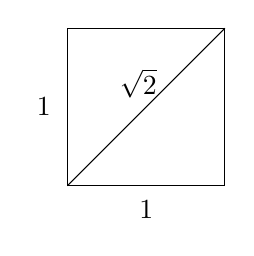
\begin{tikzpicture}
	\draw (0,0) rectangle (2,2);
	\draw (0,0) -- (2,2); 
	\node at (1,-0.3) {$1$};
	\node at (-0.3,1) {$1$};
	\node at (0.9,1.3) {$\sqrt{2}$};
\end{tikzpicture}	
\end{center}
\vspace*{-10pt}
But can you construct $\sqrt[3]{2}$?

\textbf{Modern Approach: Cartesian (Rene Descartes)} 

Plane $\longleftrightarrow$ the set of points $(x_1,x_2)$, $x_1,x_2 \in \mathbb{R}$

Line $\longleftrightarrow$ a set of points satisfying $ax_1 + bx_2 = c$ for some given $a,b,c \in \mathbb{R}$

e.g. a circle  $x_1^2 + x_2^2 = r$\\

Space $\longleftrightarrow \{(x_1,x_2,x_3)\, x_1,x_2,x_3 \iR\}$

Planes $\longleftrightarrow \{ax_1 + bx_2 + cx_3 = d\}$

Lines $\longleftrightarrow \{ax_1 + bx_2 + cx_3 = d\}$\\

\textbf{Advantages:}
\begin{enumerate}
\item Can use Analysis
\item Can do any dimension. 
\item Can replace $\mathbb{R}$ by $\mathbb{C}$ or by binary fields, i.e. $\{0,1\}$ with binary operations $1+1 = 0$. 
\end{enumerate}


 \sektion{Geometry in $\R^2$}

 $\R$ is the set of real numbers:\lecturemarker{1}{15 Jan}
 \begin{center}
 \begin{tikzpicture}
 	\draw[<->] (-4,0) -- (4,0);
 	 	\draw (-1.5,-0.08) -- (-1.5,0.08) node at (-1.5,-0.3) {$-\frac{3}{2}$};
 	\draw (0,-0.08) -- (0,0.08) node at (0,-0.3) {$0$};
 	 	\draw (1,-0.08) -- (1,0.08) node at (1,-0.3) {$1$};
 	\draw (1.44,-0.08) -- (1.44,0.08) node at (1.44,-0.3) {$\sqrt{2}$};
 	\draw (3.141,-0.08) -- (3.141,0.08) node at (3.141,-0.3) {$\pi$};
 \end{tikzpicture}	
 \end{center}

 
 
  This has the properties of being:\begin{itemize}
\item Commutative: $ab = ba$
\item Associative: $a+(b+c) = (a+b) + c	$
\item Distributive: $c(a+b) = ca + cb$
\item If $a<b,~b>0$ then $ca < cb$
\end{itemize}\vspace*{10pt}

\begin{definition}$\R^2 = $ the set of ordered pairs $(a,b)$ where $a,b \in \R$ i.e. $(a,b) \neq (b,a)$ in general. Elements of $\R^2$ are \emph{points}, or \emph{vectors}. $\mathbf{0} = (0,0) = $ origin of $\R^2$.

 A \emph{scalar} is an element of $\R$.	
\end{definition}


Properties of $\R^2$:\begin{enumerate}
\item Addition (sum): $(a,b) + (a',b') = (a+a',b+b')$
\begin{center}
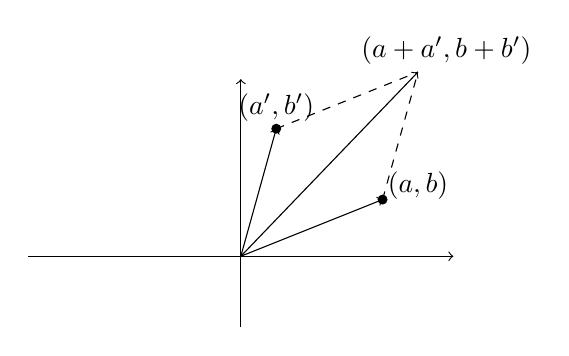
\begin{tikzpicture}[scale=.9]
	\draw[->] (-3,0) -- (3,0) node at (2.8, -0.3) {$\R$};
	\draw [->] (0,-1) -- (0,2.5) node at (-0.3,2.8) {$\R$};
	\fill (2,0.8) circle (2pt) node at (2.5,1) {$(a,b)$};
	\fill (0.5,1.8) circle (2pt) node at (0.5,2.1) {$(a',b')$};
	\draw [->] (0,0) -- (0.5,1.8);
	\draw [->] (0,0) -- (2,0.8);
	\draw [dashed] (0.5,1.8) -- (2.5,2.6);
	\draw [dashed] (2,0.8) -- (2.5,2.6) node at (2.9,2.9) {$(a+a',b+b')$};
	\draw [->] (0,0) -- (2.5,2.6);
\end{tikzpicture}	
\end{center}
\item Scalar Multiplication: If $\lambda = \R,\, (a,b) \in \R^2$, then \begin{align*}\lambda \cdot (a,b) = (\lambda a,\lambda b)\\  v \in \R^2 \implies \lambda v \in \R^2\end{align*}
\end{enumerate}
\textit{Exercise:} Check $\lambda(v_1+v_2) = \lambda v_1 + \lambda v_2$ where $\lambda \in \R,~ v_1,v_2 \in \R^2$. 

\subsektion{Lines in $\R^2$}\vspace*{5pt}

\begin{definition}
 $L$ is a \emph{line in $\R^2$}\index{Line in $RR^2$} if $\exists u, v \in \R^2~ v \neq 0$ with \[L = \{u + \lambda v ~|~ \lambda \in \R\}\]
 \end{definition}
 
 So if $u = (a_1,b_1),~v = (a_2,b_2)$ then $L = \{(a_1 + \lambda b_1, a_2 + \lambda b_2) ~|~ \lambda \in \R\}$.\\


\begin{example}~\\

\begin{minipage}{7cm}
	\begin{center}
	\begin{tikzpicture}
	\draw [->] (0,0) -- (4,0)node at (4,-0.2) {$x$};
	\draw [->] (0,0) -- (0,2.5) node at (-0.2,2.5) {$y$}; 
	\draw [->] (2.1,-0.1) -- (1,1) node at (1.2,1.2) {$L$};	
	\draw (1,1) -- (-0.1,2.1);
	\end{tikzpicture}
	
	\end{center}

\end{minipage}
\begin{minipage}{6cm}
	$x$ line is $\{(0,0) + \lambda(1,0) ~|~ \lambda \in \R\}$\\
	
	 $y$ line is $\{(0,0) + \lambda (0,1) ~|~ \lambda \in \R\}$
\end{minipage}

\vspace*{5pt}
We draw the line
  \begin{align*}L &= \{x+y = 1\}\\ &= \{(1,0) + \lambda(-1,1) ~|~ \lambda \in \R\}.\end{align*}
  
 Note that $v$ is the vector for which $L$ is parallel to.
 
Checking the components
\[
  \begin{rcases*}
  x = 1 + (-1)\lambda = 1-\lambda\;\\
  y = 0 + 1 \cdot \lambda = \lambda\; 	
  \end{rcases*}
  x+y  = 1
\]
\end{example}\vsp


Assume $L, M$ are two lines in $\R^2$, with \begin{align*}L &= \{ u = \lambda v ~|~ \lambda \in \R\},\,v \neq 0\\M &= \{a + \mu b ~|~ \mu \in \R\},\,b \neq 0\end{align*}

\begin{proposition}The two lines are the same ($L = M$) if and only if the following holds:\begin{enumerate}
\item $v = \alpha b$ for some $\alpha \in \R$
\item $L \cap M \neq \emptyset$ ($L$ and $M$ have a point in common) 	
\end{enumerate}
\end{proposition}
\begin{proof}
($\implies$)

(i) Assume that $L= M$. We know that 
\begin{align*}u \in L &\implies u \in M\\ &\implies u = a + \mu b\text{ for some }\mu \in \R\end{align*}
Also \begin{align*}
  u + v = L ~(\lambda = v) &\implies u + v \in M\\ &\implies u + v = a + \mu_1b\text{ for some }\mu_1 \in \R\\ &\implies v = (a+\mu _1b) - (a-\mu b) = (\mu _1 - \mu )b = \alpha b.
\end{align*}
(ii) Since $L=m$, surely $L \cap M = \emptyset$.\\

($\impliedby$) Assume $v = \alpha b \implies L = \{u + \lambda \alpha b ~|~ \lambda \in \R\}$. We also know that
 \begin{align*}
  L \cap M \neq \emptyset &\implies \exists c \in L \cap M\\ &\implies c \in L\\ &\implies c = u + \lambda_0\alpha b\text{, for some }\lambda_0 \in \R.
\end{align*}
Then also \begin{align*}
  c \in M &\implies c = a + \mu b\text{, for some }\mu \in \R\\ &\implies u + \lambda_0 \alpha b = a + \mu b \\&\implies u = a + \mu b - \lambda_0\alpha b = a + (\mu - \lambda_0\alpha)b \tag{$*$}
\end{align*}


Let's consider a point inside $L$:\begin{align*}
  L &= u + \lambda \alpha b \\ &= a + (\mu - \lambda_0 \alpha) b + \lambda \alpha b \quad \mbox{(using $*$)}\\ &= a + (\mu - \lambda_0 \alpha  + \lambda \alpha)b \in M
\end{align*}
 So any point in $L$ is inside $M$, so $L \subseteq M$. By symmetry $M \subseteq L \implies L = M$.
\end{proof}

\subsubsektion{Parallel Lines}

Let \begin{align*}L &= \{ u = \lambda v ~|~ \lambda \in \R\},\,v \neq 0\\M &= \{a + \mu b ~|~ \mu \in \R\},\,b \neq 0\end{align*}

\begin{definition}$L$ and $M$ are \emph{parallel} if $\exists\, \alpha \in \RR$ such that $b = \alpha v$.	
\end{definition}\vsp


\begin{proposition}
Let $x,y$ be two distinct points of $\RR^2$. Then there exists a unique line which contains both $x$ and $y$. 	
\end{proposition}

\begin{proof}
(Existence) Choose $u - x,~ v = y-x$. Then let \[L = \{x + \lambda(y-x) ~|~ \lambda \in \RR\}\] N.B. $v = y-x \neq 0$. We want to show that $x,y \in l$. Chose $\lambda = 0$, $x + \lambda(y=x) = x \in L$. Also choose $\lambda = 1$, $x + \lambda y - \lambda x = y \in L$. So $x,y$ are contained in a line. 


(Uniqueness) $L = \{u + \l v ~|~ \l \in \RR \}$. $L$ is a line through $x$ and $y$. $x \in L\implies x = u + \l_1v $
 for $\l_1 \in \RR$. $y \in L\implies y = u + \l_2v$ for $\l_2 \in \R$. 
\[y-x = (\l_2 - \l_1)v \implies v = \frac{y-x}{(\l_2 -\l_1)}\]

The vector that defined the direction of $L$ is proportional to the vector $y-x$. By the question we answered before, it's enough to show that the two lines have a point in common. $x,y$ are points in common $\implies$ Two lines are the same. 
\end{proof}


\textbf{Problem: } Construct $\sqrt{x}$. \lecturemarker{2}{16/10}
\begin{center}
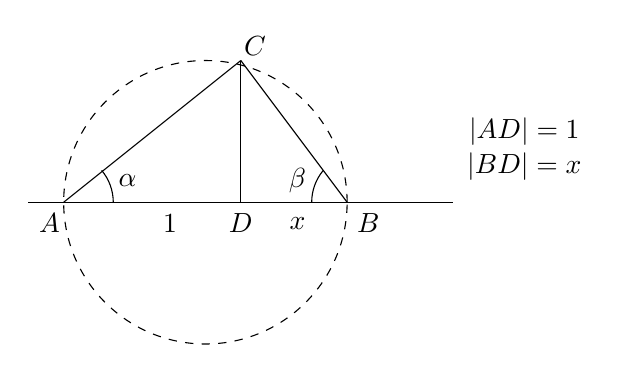
\begin{tikzpicture}[scale=.9]
\draw (0,0) -- (6,0);
\draw (3,0) -- (3,2) node at (3.2,2.2) {$C$};
\draw (0.5,0) -- (3,2) node at (0.3,-0.3) {$A$};
\draw (3,2) -- (4.5,0) node at (4.8,-0.3) {$B$};	
\draw [dashed] (2.5,0) circle (2);
\node at (2,-0.3) {$1$};
\node at (3.8,-0.3) {$x$};
\node at (3,-0.3) {$D$};
\node at (7,1) {$|AD| = 1$};
\node at (7,0.5) {$|BD| = x$};
\draw (1.2, 0) arc (0:40:0.7);
\node at (1.4, 0.3) {$\alpha$};
\draw (4, 0) arc (180:140:0.7);
\node at (3.8, 0.3) {$\beta$};
\end{tikzpicture}
\end{center}

\textbf{Claim:} $|CD| = \sqrt{x}$. 

\begin{proof}
The angle $ACD  = 90^\circ$, since $AB$ is the diameter of a circle $\implies \alpha + \beta = 90^\circ$. Note $\triangle ABC$ is similar to $\triangle DBC$, since $CAD = DCB = \alpha,\, ACD = CBD = 90^\circ$ and $CBA = CBD = \beta$. So we have a proportion: 
\begin{align*}
  \frac{|BD|}{|CD|} &= \frac{|CD|}{|AD|} \\[0.2cm]
  \frac{x}{|CD|} &= \frac{|CD|}{1} \implies |CD| = \sqrt{x}
\end{align*}
	
\end{proof}

Recall: The plane $\R^2$ is the set of vectors $(x_1,x_2),\,x_i\iR$. 

For lines  \begin{align*}L &= \{ u = \lambda v ~|~ \lambda \in \R\},\,v \neq 0\\M &= \{a + \mu b ~|~ \mu \in \R\},\,b \neq 0\end{align*}
$L ~||~ M \iff v$ and $b$ are proportional. 

$L = M \iff v$ and $b$ are proportional and they have a common point $(L \cap M \neq \emptyset$).\\

\begin{proposition}
Through any two points, there is a unique line.
\end{proposition}
\begin{proposition}
Any two non-parallel lines meet in a unique point.	
\end{proposition}
\emph{Proof.}
See exercise sheet.\\

\begin{example}
Let \vspace*{-5pt}\begin{align*}
  L = \{(0,1) + \lambda(1,1)\}\\
  M = \{(4,0) + \mu(2,1)\}
\end{align*}
The common point $ = (0,1) + \lambda(1,1) = (4,0) + \mu(2,1)$. 

Equating $x$ and $y$'s, we see from the first co-ordinate: $\lambda = 4 + 4\mu$. From the second co-ordinate: $1 + \lambda = \mu$.

So \vspace*{-5pt}
\begin{align*}
  \lambda &= 4 + 2(\lambda + 1) \\
  \implies \lambda &= -6
\end{align*}
Therefore the common point is $(-6,-5)$. 
\end{example}






\subsektion{Triangles}\vsp
\begin{definition}
A triangle is a set of $3$ points in $\R^2$ that are not on a common line.	
\end{definition}
\begin{center}
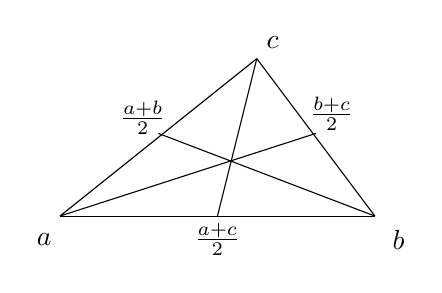
\begin{tikzpicture}
\draw (0.5,0) -- (4.5,0);
\draw (2.5,0) -- (3,2) node at (3.2,2.2) {$c$};
\draw (0.5,0) -- (3,2) node at (0.3,-0.3) {$a$};
\draw (3,2) -- (4.5,0) node at (4.8,-0.3) {$b$};	
\node at (2.5,-0.3) {$\frac{a+c}{2}$};
\draw (0.5,0) -- (3.75,1.05) node at (3.95,1.3) {$\frac{b+c}{2}$};
\draw (4.5,0) -- (1.75,1.05) node at (1.55,1.25) {$\frac{a+b}{2}$};
\end{tikzpicture}
\end{center}

\begin{definition}[Midpoint]
The \emph{midpoint} of $ab$ is the vector $\frac{1}{2}(a+b)$.	
\end{definition}

\begin{definition}[Median]
A \emph{median} is the line joining a corner to the midpoint of the opposite side.
\end{definition}\vsp

\begin{proposition}
The three medians of the triangle meet in a common point.	
\end{proposition}

\begin{proof}
The medians are 
\begin{align*}
  L_a &=\textstyle{ \{a + \lambda(\frac{b+c}{2} -a )\}}\\
  L_b &=\textstyle{ \{b + \lambda(\frac{a+c}{2} -b )\}}\\
  L_c &=\textstyle{ \{c + \lambda(\frac{a+b}{2} -c )\}}
\end{align*}	
We can write them as
\begin{align*}
  L_a =\{ \textstyle{(1-\lambda)a + \frac{\lambda}{2}b + \frac{\lambda}{2}c\}}\\
  L_b = \{\textstyle{(1-\mu)b + \frac{\mu}{2}a + \frac{\mu}{2}c}\}
\end{align*}
Take $\lambda = \mu$, then $\frac{\mu}{2}c = \frac{\lambda}{2}c$. Also $\frac{\lambda}{2} = 1-\mu = 1-\lambda \implies \lambda = \frac{2}{3}$. Hence $L_a = L_b$. 

Check: $\lambda = \frac{2}{3} \implies L_a = L_b$. So the common point is $\frac{1}{3}(a + b + c) \in L_a \cap L_b \cap L_c$. 
\end{proof}\vsp

\begin{definition}[Distance]
	The \emph{length} of a vector $x = (x_1,x_2)$ is $\sqrt{x_1^2 + x_2^2}$. We denote the length of $x$ by $||x|| = \sqrt{x_1^2 + x_2^2}$. 
	
	The \emph{distance} between two points $x,y\iR^2$ is 
	\[||x-y|| = \sqrt{(x_1-y_1)^2 + (x_2-y_2)^2}\]
\end{definition}\vsp

\begin{definition}[Scalar product]
The \emph{scalar product} (or dot product) of two vectors $x,y\iR^2$ is 
\[(x\cdot y) = x_1y_1 + x_2y_2\]	
\end{definition}

E.g. If $x = (1,-1),\, y= (1,2)$ then $(x\cdot y) = 1 + (-2) = -1$. 

Easy properties: For any vectors $x,y,z \iR^2$
\begin{itemize}
\item $x\cdot (y + z) = x\cdot y + x\cdot z$ (distribution over $+$)
\item $||x||^2 = (x\cdot x) = x_1^2 + x_2^2$
\item $(x\cdot y) = (y\cdot x)$ (commutativity)	
\end{itemize}\vsp



\begin{proposition}[Cauchy-Schwartz Inequality]
For $x,y \iR^2$ {\normalfont \lecturemarker{3}{17/10}}
\[|(x\cdot y)| \leq ||x|| \cdot ||y||\]
With equality iff $x,y$ are multiples of the same vector. 
\end{proposition}
\begin{proof}
%Let $\lambda$ be any real number. Consider $x-\lambda y$ and obverse that 
%\[
%\begin{aligned}
%  ||x -\lambda y||^2 \geq 0 &\implies (||\lambda||^2 - \lambda^2||y||^2 -2x \lambda y) \geq 0\\
%  &\implies ||y||^2 \cdot \lambda^2 - 2\lambda(x\cdot y) + ||x||^2 \geq 0
%\end{aligned}
%\]
%If we let $a = ||y||^2$, $b = -2\lambda(x\cdot y)$ and $c = ||x||^2$, then $a\lambda^2 + b\lambda+c \geq 0$ for any $\lambda$ implies the discriminant, $b^2 - 4ac \leq 0 \implies 4(x\cdot y)^2 \leq 4||x||^2 - ||y||^2$. 
w.l.o.g. $y \neq (0,0)$. Consider all vectors of the form $x -\lambda y$. The length $||x-\lambda y||$ squared is clearly $\geq 0$, so 
\begin{align*}
  ||x-\lambda y||^2 &= (x-\lambda y \cdot x -\lambda y)\\
  &= (x\cdot x) - 2\lambda(x\cdot y) + \lambda^2(y\cdot y)\\
  &= ||x||^2 - 2\lambda(x\cdot y) + \lambda^2||y|| \geq 0
\end{align*}
This is a quadratic polynomial in $\lambda$ with real coefficients and at most one real root $(=0)$. Now 
\begin{align*}
  \lambda^2 ||y||^2 - 2\lambda(x\cdot y) + ||x||^2 \geq 0 &\implies \text{ discriminant, }D \leq 0\\
  &\implies ((2(x\cdot y))^2 \leq 4||x||^2||y||^2\\
  &\implies 4(x\cdot y)^2 \leq 4||x||^2||y||^2\\
  &\implies |x\cdot y| \leq ||x||||y||
\end{align*}

	
The equality condition is clear for $y=0$. Assume that $y$ is not the zero vector. If $|(x\cdot y)|^2 = ||x|| \cdot ||y||$, then $D = 0$. \[D = 4(x\cdot y)^2 -4||x||^2 \cdot ||y||^2 =0\] Then $a\lambda^2 + b\lambda +c$ has a double root, say $\lambda_0$. But $a\lambda_0^2 + b\lambda_0 + c= ||x-\lambda_0y||^2 = 0$. Therefore $x-\lambda_0y$ is the zero vector. Thus $x = \lambda_0y$. 			
\end{proof}\vspace*{5pt}

\begin{proposition}[Triangle Inequality]
For any vectors $x,y \iR^2$, we have 
\[||x+y|| \leq ||x|| + ||y||\]
If equality holds, then $x$ and $y$ are multiples of the same vector. 
\end{proposition}

\begin{center}
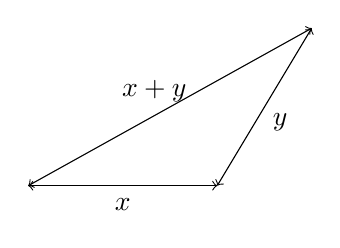
\begin{tikzpicture}[scale=.8]
\draw[<->] (0,0) -- (3,0) node at (1.5,-0.3) {$x$};
\draw[<->] (3,0) -- (4.5,2.5) node at (4,1) {$y$};
\draw[<->] (0,0) -- (4.5,2.5) node at (2,1.5) {$x + y$};	
\end{tikzpicture}
	
\end{center}

\begin{proof}
It is enough to prove that the square on LHS $\leq$ RHS, i.e. 
\[
  ||x+y||^2 \leq ||x||^2 + ||y||^2 + 2||x||\cdot||y||
\]
We've already seen that 
\[
  ||x+y||^2 = (x+y\cdot x+y) = ||x||^2 + ||y||^2 + 2(x\cdot y)
\]
By Cauchy-Schwartz $(x\cdot y) \leq ||x||\cdot ||y||$, hence the inequality is proved. To prove the equality condition, we note that the triangle inequality is an equality precisely when $(x\cdot y) = ||x|| + ||y||$. By Theorem 1.4, we conclude that $x$ and $y$ are multiples of the same vector. 
\end{proof}

Recall the scalar product of $x$ as $||x||^2 = (x\cdot x)$. The scalar product can be reconstructed if we only know the lengths of vectors:\\

\begin{proposition}
For any two vectors $x,y \iR^2$, we have 
\[
  (x\cdot y) = \frac{1}{2}(||x||^2 + ||y||^2 - ||x-y||^2)
\]

\end{proposition}

\begin{proof}
\[
\begin{aligned}
  RHS &= \frac{1}{2}(||x||^2 + ||y||^2 - ||x||^2 - ||y||^2 + 2(x\cdot y)\\
  &= (x\cdot y)
\end{aligned}
\]
\end{proof}

\subsektion{Angles}

From the Cauchy-Schwartz inequality, we find that $-1 \leq \dfrac{(x\cdot y)}{||x||\cdot||y||}\leq 1$. \\[.2cm]

\begin{definition}
	We define $\theta$ as the angle such that $\cos\theta = \dfrac{(x\cdot y)}{||x|| \cdot||y||}$
\end{definition}

\begin{center}
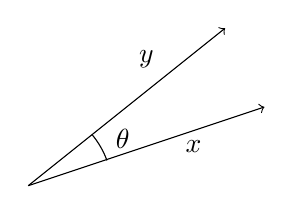
\begin{tikzpicture}
\draw [->] (0,0) -- (3,1) node at (2.1,0.5) {$x$};
\draw[->] (0,0) -- (2.5,2) node at (1.5,1.6) {$y$};
\draw (1, 0.32) arc (20:40:1.1);
\node at (1.2, 0.6) {$\theta$};
\end{tikzpicture}
\end{center}

In particular, $x$ and $y$ are perpendicular iff $(x\cdot y) = 0$. 

Lines in $\R^2$ can be written as $L =\{u + \lambda v ~|~ \lambda \iR\}$. This will be referred to as \emph{vector form}. Lines can also be described by their \emph{Cartesian equation}: $px_1 + qx_2 + r = 0$, where $p_1,q_1 \iR$.\\

\begin{definition}
Any vector perpendicular to the direction vector of a line is called a \emph{normal} vector to $L$. 
\end{definition}


\begin{center}
\begin{tikzpicture}
\draw [->] (0,0) -- (4,1.5) node at (2.1,0.5) {$L$};
\draw [dashed,->] (1.5,0.5) -- (1,1.7) node at (0.8,1.5) {$n$};
\end{tikzpicture}
\end{center}



If $L = \{u +\lambda v\},\; v = (v_1,v_2)$, then $n = (-v_2,v_1)$ is a normal vector to $L$. 

\emph{Remark.} Let $n\iR^2$ be any (non-zero) normal vector to $L= \{u + \lambda v\}$. Then all points $x \in L$ have the property that $(x\cdot n)$ is constant. Indeed, $x = u + \lambda v$, hence 
\[
  (x\cdot n) = ((u +\lambda v)\cdot n) = (u\cdot n) + \underbrace{\lambda(v\cdot n)}_{=\,0} = u \cdot n.
\]
Therefore every point $x$ of $L$ satisfies the equation $n_1x_1 + n_2x_2 = c$, where $c$ is a constant ($c = u_1n_1 + u_2n_2$). $L$ can be given by $-v_2x_1 + v_1x_2 = c$ for some $c$. \\


\subsubsektion{From Cartesian to Vector form}
Start with $L$ which is the zero set of $px_1 + qx_2 + r = 0$. Now $(p,q)$ is a normal vector to $L$, hence $v = (q,-p)$ is a possible direction vector of $L$. ($(-q,p)$ is another possibility.) Then $L = \{u + \lambda v~|~ \lambda\iR\}$ for an appropriate vector of $a$. $px_1 + qx_2 + r = 0$. ($(p,q)\cdot x)=$ constant. (this constant is $-r$). 

The lines $L = \{u +\lambda v\}$ and $M = \{a + \mu b\}$ are perpendicular iff $(v\cdot b) = 0$. The lines $px_1 + qx_2 +r = 0$ and $ex_1 + fx_2 + g = 0$ are perpendicular iff the normal vectors to these lines e.g. $(p,q)$ and $(e,f)$ are perpendicular. This happens when $(p,q) \cdot (e,f) = 0$.\\ 

\textbf{Claim:} The \lecturemarker{4}{21/10} vector $(p,q)$ is a normal vector to $L$, given by $px_1 + qx_2 + r = 0$.

\begin{proof}
We must show that $(p,q)$ is perpendicular to $(x-y)$, where $x \in L$ and $y \in L$. 

Consider

\begin{minipage}{7cm}
	\begin{center}
	\begin{tikzpicture}
	\draw[->] (0,0) -- (-2,-1) node at (-2,-0.7) {$x$};
	\draw (-2,-1) -- (-3,-1.5);
	\fill (-1,-0.5) circle (2pt) node at (-1,-0.2) {$y$};	
	\end{tikzpicture}
	
	\end{center}
\end{minipage}
\begin{minipage}{5cm}
\[  px_1 + qx_2 + r = 0 \tag{1}\]
\[  py_1 + qy_2 + r = 0 \tag{2}\]

\end{minipage}

\[
\begin{aligned}
  (1) - (2): p(x_1-y_1) + q(x_2 - y_2) &= 0\\
  \implies (p,q)\cdot(x_1-y_1,x_2-y_2) &= 0
\end{aligned}
\]
Hence $(p,q) \cdot(x-y) = 0$. So that $(p,q)$ is perpendicular to $(x-y)$.
\end{proof}


\vspace*{2.5cm}



\begin{center}

\includegraphics[width=8cm]{cartoon3.jpg}
\end{center}




\sektion{Matrices}\vsp

\begin{definition}Let $n$ be a natural number, $n = 1,2,3,\dots$. Then $\R^n$ is the set of all vectors with $n$ co-ordinates $(x_1,\dots,x_n)$. \end{definition}
E.g. $\R$ is the real line. $\R^2$ is the real plane. $\R^3$ is 3-dimensional space etc.\\	


\begin{definition}[Vector Operations]

Vector addition:\[
\begin{aligned}
 &(x_1,x_2,\dots,x_n) + (y_1,y_2,\dots,y_n)\\
  &= (x_1 + y_1,x_2 + y_2,\dots,x_n+y_n)
\end{aligned}
\]

Multiplication by scalar $\alpha\iR$: \[\alpha(x_1,\dots,x_n) = (\alpha x_1,\dots,\alpha x_n)\]

Dot product of two vectors: \[(x_1,\dots,x_n)\cdot(y_1,\dots,y_n) = (x_1y_1 + x_2y_2 + \dots x_ny_n)\]
\end{definition}

\subsektion{System of Linear Equations}

A linear equation of $n$ vairables is of the form $a_1x_1 + \dots a_nx_n = b$, where $a_1,\dots,a_n,b\iR$. We want to solve systems of such linear equations.\\

\begin{example}
\begin{align*}
x_1 + x_2 &= 3 \tag{1}\\
-2x_1 + x_2 &= 1\tag{2}	
\end{align*}

$2 * (1) + (2)$ elimated $x$, leaving $3x_2 = 7 \implies x_2 = \frac{7}{3}$. Then $x_1 = 3-x_2 = \frac{2}{3}$. 
	
\end{example}\vspace*{5pt}

\begin{example}
\begin{align*}
  x_1 - 2x_2 &= 2 \tag{1}\\
  3x_1 - 6x_2 &= 4\tag{2}
\end{align*}
$-3\times (1) + 2$ is $0= -2$. So this system has no solutions. 
\end{example}\vspace*{5pt}

\begin{example}
\begin{align*}
  x_1 + x_2 &= 0 \tag{1}\\
  x_2 - x_3 &= 0 \tag{2}\\
  x_1 - x_2 + 2x_3 &= 0\tag{3}
\end{align*}

Observe $(3) = (1) - 2\times(2)$. So $(1)$ and $(2)$ are enough here, so $(3)$ is automatically satisfied if $(1)$ and $(2)$ are satisfied. So $x_3 = a \iR$, any real number. Then $(2)$ says that $x_2 = a$. Then $(1)$ says that $x_1 = -a$. So this system has infinitely many solutions, which are $(-a,a,a)$ for any $a\iR$. 
\end{example}\vspace*{5pt}

Consider a general system of linear equations of $n$ variables $x_1,\dots,x_n$: 
\begin{align*}
  a_{11}x_1 + a_{12}x_2 +\dots + a_{1n}x_n &= b_1\\
  a_{21}x_1 + a_{22}x_2 + \dots + a_{2n}x_n &= b_2\\
  \vdots\\
  a_{m1}x_1  + a_{m2}x_2 + \dots + a_{mn}x_n &= b_m
\end{align*}

A vector $(y_1,\dots,y_n),\, y_i \iR$ is a solution of the system if all the equations are satisfied when we put $x_1 = y_1,\dots,x_n = y_n$.

\subsektion{Gaussian Elimination}\vspace*{10pt}

\begin{example}
\begin{align*}
  x_1 + 2x_2 + 3x_3 &= 9 \tag{1}\\
  4x_1 + 5x_2 + 6x_3 &= 24 \tag{2}\\
  3x_1 + x_2 - 2x_3 &= 4\tag{3}
\end{align*}
	
\textsc{Step 1:} Eliminate $x_1$ from $(2)$ and $(3)$. We replace $(2)$ by $(2) - 4\times(1)$ and replace $(3)$ by $(3) - 3 \times(1)$. We obtain:
\begin{align*}
  x_1 + 2x_2 + 3x_3 &= 9\\
  -3x_2 -6x_3 &= -12\\
  -5x_2 -11x_3 &= -23
\end{align*}

\textsc{Step 2:} Make the coefficent of $x_2$ in $(2)$ equal to $1$.
\begin{align*}
  x_1 + 2x_2 + 3x_3 &= 9\\
  x_2 + 2x_3 &= 4\\
  -5x_2 - 11x_3 &= -23
\end{align*}

\textsc{STEP 3:} Eliminate $x_2$ from equation $(3)$ by adding $5 \times(2)$ to $(3)$: 
\begin{align*}
  x_1 + 2x_2 + 3x_3 &= 9\\
  x_2 + 2x_3 &= 4\\
  -x_3 &= -3
\end{align*}

\textsc{Step 4:} Make the coefficient of $x_3 = 1 \implies x_3 = 3$. 

\textsc{Step 5:} Work backwards to obtain first $x_2$ from $(2)$ and then $x_1$ from $(1)$. $\implies x_2 = 4-2x_3 = -2$ and $x_1 = 9-2x_2 -3x_3 = 4$. Finally we've solved the system and we have found all the solutions of the system. 
\end{example}


\subsektion{Matrices}\vspace*{5pt}

\begin{definition}A $m\times n$ matrix is a rectangular array of $mn$ real numbers, arranged into $m$ rows and $n$ columns. 
\[
  \begin{pmatrix}
  a_{11} & a_{12} &\dots & a_{1n} \\
  a_{21} & a_{22} & \dots &a_{2n}\\
  \vdots & & & \vdots\\
  a_{m1} & a_{m2} & \dots &a_{mn}	
  \end{pmatrix}
\]
The matrix entry is written down as $a_{ij}$ where $i$ is the number of the row and $j$ is the number of the column. Sometimes this matrix is denoted by $(a_{ij})$ or $(a_{ih}) 1 \leq 1 \leq m,\,1\leq j \leq n$. 
\end{definition}

\subsubsektion{Basic examples of matrices}
- Any $n$-dimensional vector is a matrix of size $1\times n$. $(1,\dots, n$) is a matrix with one row.

- A column vector is $\left(\begin{smallmatrix}
x_1\\x_2\\\vdots\\x_m	
\end{smallmatrix}\right)$. This is a matrix of size $m\times 1$. 

\textbf{Other examples}

- $\begin{pmatrix}
1 & -1 & 5\\ 2 & 0 & 1	
\end{pmatrix}
$ has size $2 \times 3$ and $\begin{pmatrix}
2 & 5\\ 6 & 7\\ 0 & 3	
\end{pmatrix}$ has size $3\times 2$. 

- $\begin{pmatrix} 
1 & 0 & 0 &0 \\
0 & 1 & 0 & 0 \\
0 & 0 & 1 & 0 \\
0 & 0 & 0 &1	
\end{pmatrix}
$ is the \emph{identity matrix} (of size $4\times 4$). 

A matrix such that $m = n$ is called a \emph{square matrix.} 

To our general linear system we attach its co-efficient matrices:
\begin{align*}
 & \begin{pmatrix}
  a_{11} & a_{12} &\dots & a_{1n} \\
  a_{21} & a_{22} & \dots &a_{2n}\\
  \vdots & & & \vdots\\
  a_{m1} & a_{m2} & \dots &a_{mn}	
  \end{pmatrix}
 \;\text{ and }\;
 \begin{pmatrix}
 b_1\\ \vdots\\ b_m	
 \end{pmatrix}\\[0.5cm]
  \implies & \begin{pmatrix}
  a_{11} & a_{12} &\dots & a_{1n} & b_1 \\
  a_{21} & a_{22} & \dots &a_{2n} & b_2\\
  \vdots & & & \vdots\\
  a_{m1} & a_{m2} & \dots &a_{mn} &b_m	
  \end{pmatrix} \text{, the \emph{augmented matrix}.}
\end{align*}

\begin{definition}[Elementary Row Operations]\lecturemarker{5}{blah}
The following operations are the \emph{elementary row operations}. 
\begin{enumerate}
\item Add a scalar multiple of one row to another: $r_i \longrightarrow r_i + \lambda r_j,\; \lambda\iR$. 
\item Swap two rows $(r_i \leftrightarrow r_j$)
\item Multiply a row by a non-zero number: $r_i \longrightarrow \lambda r_i,\; \lambda\iR,\,\lambda\neq 0$. 	
\end{enumerate}	
\end{definition}

Point: The new equations are combinations of the old ones, and vice-versa, so that the set of solutions is exactly the same.\\

\setcounter{equation}{3}
\begin{example}[Revisited]
\[
  \begin{pmatrix}
   1 & 2 & 3 & 9\\
   4 & 5 & 6 & 24\\
   3 & 1 & -2 & 4	
  \end{pmatrix}
\]

\textsc{Step 1:} $r_2 \longrightarrow r_2 -4r_1$, $r_3 \longrightarrow r_3-3r_1$. 
\[
  \begin{pmatrix}
  1 & 2 & 3 & 9 \\
  0 & -3 & -6 & -12\\
  0 & -5 & -11 & -23	
  \end{pmatrix}
\]

\textsc{Step 2:} $r_2 \longrightarrow -\frac{1}{3}r_2$.
\[
  \begin{pmatrix}
  1 & 2 & 3 & 9\\
  0 & 1 & 2 & 4\\
  0 & -5 & -11 & -23	
  \end{pmatrix}
\]

\textsc{Step 3:} $r_3 \longrightarrow r_3 + 5r_2$. 
\[
  \begin{pmatrix}
  1 & 2 & 3 & 9\\
  0 & 1 & 2 & 4\\
  0 & 0 & -1 & -3	
  \end{pmatrix}
\]

\textsc{Step 4:} $r_3 \longrightarrow -1r_3$\\[0.1cm]
\begin{minipage}{6cm}
\[\hspace*{3cm}
\underbrace{\begin{pmatrix}
  1 & 2 & 3 & 9\\
  0 & 1 & 2 & 4\\
  0 & 0 & 1 & 3
  \end{pmatrix}}_{\text{Echelon form}}
\]
\end{minipage}
\begin{minipage}{3cm}
\begin{align*}
	x_1 + 2x_2 + 3x_3 &= 9\\
  \implies \qquad \qquad x_2 + 2x_3 &= 4\\
  x_3 &= 3
\end{align*}
\vspace*{10pt}
	
\end{minipage}

\end{example}\vspace*{5pt}

\begin{definition}
A matrix is in \emph{echelon form} if 
\begin{enumerate}
\item The first non-zero entry in each row is appears to the right on the non-zero entry in all the rows above
\item All rows consiting only of zeros $(0,0,\dots,0)$, if any, appear at the bottom. 	
\end{enumerate}
\end{definition}

\textbf{Examples of echelon form:} 
\[
  \begin{pmatrix}
  0 & 1 & 5 & 0\\
  0 & 0 & 5 & -3	
  \end{pmatrix}
  \; \text{ Yes } 
  \qquad 
  \begin{pmatrix}
  6 & 2 & 4 & 0\\
  0 & 0 & 1 & 5\\
  0 & 0 & 0 & 0	
  \end{pmatrix}
  \; \text{ Yes}
\]

\textbf{Non-examples}
\[
  \begin{pmatrix}
  0 & 1 & 17\\
  1 & 0 & 2	
  \end{pmatrix}
 \; \text{ No} 
 \qquad 
 \begin{pmatrix}
 0 & 1 & 17\\
 0 & 1 & 5	
 \end{pmatrix}
 \; \text{ No} \qquad
 \begin{pmatrix}
 0 & 0 & 0\\
 1 & 2 & 5\\
 0 & 1 & 2	
 \end{pmatrix}\; \text{ No} 
\]

\emph{Remark.} If we reduce the augmented matrix of a system of linear equations to the echelon form, then we can easily solve it.\\

\begin{example}
\[
  \begin{pmatrix}
  1 & -1 & 3 & 0\\
  0 & 1 & 1 & 1\\
  0 & 0 & 0 & 0	
  \end{pmatrix}
\]
If we have a row $(0,\dots,0,a)$ where $a \neq 0$ then there are no solutions. We say that the linear system is \emph{inconsistent} since $0\cdot x_1 + 0 \cdot x_2 + \dots 0\cdot x_n = a$. 

Now ignore all zero-rows. To solve this linear system, we start at the bottom: $x_2 + x_3 = 1$. $x_3 =a$, where $a$ is any real number. $x_1 = 1-a$. 

Express the variable corresponding to the first non-zero entry in this row in terms of the variables that come after it. $x_1 - x_2 + 3x_3 = 0$. Thus $x_1 = x_2 - 3x_3= 1-a - 3a = 1-4a$. The general solution is $(1-4a,1-a,a),a \iR$. The variables that are assigned arbitrary values are called \emph{free variables}, and all other variables are \emph{dependent} variables. 
\end{example}\vspace*{5pt}

\begin{example}
\[
  \begin{pmatrix}
  1 & -1 & 3 & 0 \\
  0 & 1 & 1 & 1\\
  0 & 0 & 0 & 2	
  \end{pmatrix}
\]
$0\cdot x_1 + 0\cdot x_2 + 0\cdot x_3 = 2$. This is inconsistent, so no solutions.
\end{example}\vspace*{5pt}

\begin{example}
\[\begin{pmatrix}
1 & 1 & 1 & 3 & 2 & 4 & 0\\
0 & 0 & 0 & 1 & -1 & 0 & 3\\
0 & 0 & 0 & 0 & 1 & 1 & 0	
\end{pmatrix}\]

$x_5 + x_6 = 0$, so let $x_6 = a,\, a\iR$. Then $x_5 = -a$. $x_4 - x_5 = 3 \implies x_4 = 3-a$. 

$x_1 + x_2 + x_3 + 3x_4 + 2x_5 + 4x_6 = 0$. We get new free variables: $x_2 = b, b\iR$ and $x_3 = c$, for any $c\iR$. $\implies x_1 = -b -c + a -9 \implies (a-b-c-9,\, b,\, c,\, -a -3,\, -a,\,a)$.
\end{example}\vspace*{5pt}

\begin{theorem}[Gaussian Elimination]
	Any matrix can be reduced to a matrix in echelon form by elementary row operations.
\end{theorem}

Example: 
\[
  \begin{pmatrix}
  1 & 0 & 3 & 2 & 5 & 1\\
  1 & 0 & 3 & 5 & 8 & 1\\
  1 & 1 & 4 & 5 & 7 &0\\
  1 & -1 & 2 & -1 & 3 & 2 	
  \end{pmatrix}
\]
Step 1: Clear the first column. 
\[
  \begin{pmatrix}
  1 & 0 & 3 & 2 & 5 & 1\\
  0 & 0 & 0 & 3 & 3 & 0 \\
  0 & 1 & 1 & 3 & 2 & -1\\
  0 & -1 & -1 & -3 & -2 & 1
  \end{pmatrix}
\]
Step 2: Swap 2nd row with 4th row
\[
  \begin{pmatrix}
  1 & 0 & 3 & 2 & 5 & 1\\
  0 & -1 & -1 & -3 & -2 & 1\\
  0 & 1 & 1 & 3 & 2 & -1\\
  0 & 0 & 0 & 3 & 3 & 0	
  \end{pmatrix}
\]
Step 3: $r_3 \longrightarrow r_2 + r_3$
\[
  \begin{pmatrix}
  1 & 0 & 3 & 2 &5 & 1\\
  0 & 1 & 1 & 3 & 2 & 1\\
  0 & 0 & 0 & 0 & 0 & 0 \\
  0 & 0 & 0 & 3 & 3 & 0	
  \end{pmatrix}
\]
and we're done. 

Now for the proof of the theorem: 

\begin{proof}
Let\lecturemarker{6}{24/10}
$A = \begin{pmatrix}	
a_{11} &\dots & a_{1n}\\
a_{21} &\dots & a_{2n}\\
\vdots & & \vdots\\
a_{m1} & \dots & a_{mn}
\end{pmatrix}
$ be an arbitrary $m\times n$ matrix. 

The basic procedure consists of two steps: 

\textsc{Step 1:} Find a non-zero entry furthest to the left in $A$. So $A$ looks like this: 
\[
  \begin{pmatrix}
  0 & 0 &\dots & 0 & * &\dots \\
  0 & 0 &\dots & 0 & * &\dots \\
  \vdots & \vdots &&\vdots & * & \\
    0 & 0 &\dots & 0 & * &\dots \\
  \end{pmatrix}
\]
If this non-zero element is in the row with number $j$, then swap the first row with the $j$-th row $(r_i \leftrightarrow r_j$). Multiply this new row $1$ to make this non-zero element equal to $1$. 

Outcome of Step 1: 
\[
  \begin{pmatrix}
    0 &\dots & 0 & 1 &\dots &* \\
    0 &\dots & 0 & * &\dots &*\\
  \vdots &&\vdots & * && \\
     0 &\dots & 0 & * &\dots &*\\
  \end{pmatrix}
\]

\textsc{Step 2} Subtracting multiples of the first row from other rows to ensure that then entries underneath this $1$ are all equal to $0$. 

Outcome of Step 2:  

 \begin{center}
      \begin{tikzpicture}
        \matrix [matrix of math nodes,left delimiter=(,right delimiter=)] (m)
        {
  		 0 &\dots & 0 & 1 & * & \dots &* \\
  		 0 &\dots & 0 & 0 &  *  & \dots &*\\
   		 \vdots &&\vdots & \vdots &  & A_1& \\
   		 0 &\dots & 0 & 0 & * &\dots &*\\
        };  
        \draw[color=red] (m-2-5.north west) -- (m-2-7.north east) -- (m-4-7.south east) -- (m-4-5.south west) -- (m-2-5.north west);
    \end{tikzpicture}
    \end{center}

From now on we only use row operations involving rows from $2$ to $m$. (never use row $1$ anymore). We'll apply steps 1 and 2 to the ``red" matrix $A_1$. ($A_1$ is $A$ with the first $j$ columns and 1st row removed). The outcome of  steps 1 and 2 applied to $A_1$ is:

 \begin{center}
      \begin{tikzpicture}
        \matrix [matrix of math nodes,left delimiter=(,right delimiter=)] (m)
        {
        0 & \dots & 0 & 1 & * & \dots & * & *\\
  		 0 &\dots & 0 & 0 & 1 & \dots &* &*\\
  		 0 &\dots & 0 & 0 &  0  & * & \dots &*\\
   		 \vdots &&\vdots & \vdots & \vdots  & & A_2&\\
   		 0 &\dots & 0 & 0 & 0 &* &\dots &*\\
        };  
        \draw[color=red] (m-3-6.north west) -- (m-3-8.north east) -- (m-5-8.south east) -- (m-5-6.south west) -- (m-3-6.north west);
    \end{tikzpicture}
    \end{center}


Let us now consider $A_2$ and repeat steps 1 and 2 for $A_2$ and so on. The number of rows of $A_1$ is $m-1$, the number of rows of $A_2$ is $m-2,\dots$. Hence after finitely many iterations, we'll stop. In the end the matrix will be in the echelon form!
% \begin{center}
%      \begin{tikzpicture}
%        \matrix [matrix of math nodes,left delimiter=(,right delimiter=)] (m)
%        {
%        0 & \dots & 0 & 1 & * & \dots & * & *\\
%  		 0 &\dots & 0 & 0 & 1 & \dots &* &*\\
%  		 0 &\dots & 0 & 0 &  0  & 1 & \dots &*\\
%   		 \vdots &&\vdots & \vdots & \vdots  & \vdots &  &1\\
%   		 0 &\dots & 0 & 0 & 0 & 0 &\dots &0\\
%        };  
%    \end{tikzpicture}
%    \end{center}
\end{proof}



\sektion{Matrix Algebra}

\begin{definition}
The \emph{zero matrix} of size $m \times n$ is 
\[0 = \begin{pmatrix}
 0 & \dots & 0\\
 0 & \dots & 0\\
 0 & \dots & 0	
 \end{pmatrix}
\]
\end{definition}

\subsubsektion{Addition}

If $A$ and $B$ are both $m \times n$ matrices, with entries $a_{ij}$ and $b_{ij}$ respectively, then $A+B$ is the matrix of size $m \times n$ with entries $a_{ij} + b_{ij}$: 
\[
  \begin{pmatrix}
  a_{11}+b_{11} & \dots & a_{1n} + b_{1n}\\
  \vdots & & \vdots\\
  a_{m1} + b_{m1} & \dots   & a_{mn} + b_{mn}
  \end{pmatrix}
\]\vspace*{5pt}

\subsubsektion{Multiply matrices by a scalar:}

If $c \iR$ and $A$ is a matrix of size $m \times n$, with $A= (a_{ij})$ then $cA$ is the matrix of size $m \times n$ with entries $(ca_{ij})$. 
\[
  \text{ If }
  A = \begin{pmatrix}
  a_{11} & a_{12}\\
  a_{21} & a_{22}
\end{pmatrix}
\qquad cA = 
\begin{pmatrix}
  ca_{11} & ca_{12}\\
  ca_{21} & ca_{22}
\end{pmatrix}
\]

\subsubsektion{Matrix Multiplication:} 

Let $A$ be a matrix of size $m \times n$ and $B$ a matrix of size $n \times k$. Then $AB$ is a matrix of size $m \times k$ defined as follows: 
\[
  B =\begin{pmatrix}
  \uparrow & \uparrow & & \uparrow\\
  c_1(B) & c_2(B) & \dots & c_k(B)\\
  \downarrow & \downarrow & & \downarrow
\end{pmatrix}
\qquad 
A = \begin{pmatrix}
 \leftarrow & r_1(A) & \rightarrow \\
 \leftarrow & r_2(A) &  \rightarrow\\
 	&\vdots & \\
  \leftarrow & r_k(A) &  \rightarrow\\
 \end{pmatrix}
\]

Each if the row vectors $r_i(A)$ has $n$ co-ordinates. Each of the column vectors $r_i(B)$ has $n$ co-ordinates. Because each of $r_i(A)$ and $c_j(B)$ has exactly $n$ co-ordinates, we can form the dot product $r_i(A) \cdot c_j(B)$ for any $1 \leq i \leq m\; 1 \leq j \leq k$. The $ij-$entry of $AB$ is defined to be the dot prodcut $r_i(A) \cdot c_j(B)$.\\

\begin{examples}
\begin{enumerate}
\item $1 \times 1$ matrices are just a number, so if $A = (a)$ and $B = (b) \implies AB = (ab)$. 
\item $2\times 2$ matrices, $A = \left(\begin{smallmatrix}
a_{11} & a_{12} \\ a_{21} & a_{22}	
\end{smallmatrix}\right)$, $B = \left(\begin{smallmatrix}
b_{11} & b_{12} \\ b_{21} & b_{22}	
\end{smallmatrix}\right)$, then 
\[
  AB = \begin{pmatrix}
  a_{11}b_{11} + a_{12}b_{21} & a_{11}b_{12} + a_{12}b_{22}\\
  a_{21}b_{11} + a_{22}b_{21} & a_{21}b_{12} + a_{22}b_{22}
\end{pmatrix}
\]
\item $A = (a_{11},\,a_{12},\dots,a_{1n})$ a $1\times n$ matrix and $B = \left(\begin{smallmatrix} b_{11}\\\vdots \\ b_{n1}\end{smallmatrix}\right)$ then 
\[
AB = (a_{11}b_{11} + a_{12}b_{21} + \dots + a_{1n}b_{n1})  
\]
(which is a $1\times 1$ matrix, i.e. a number)

\item $BA$ will be a matrix of size $n \times m:$
\[\left(
  \begin{smallmatrix}
  b_{11} \\ b_{21} \\ \vdots \\ b_{n1}	
  \end{smallmatrix}\right)
  (a_{11},\,a_{12},\,\dots ,\,a_{1n}) = 
  \begin{pmatrix}
  	b_{11}a_{111} &  \dots & b_{11}a_{1n}\\
  	b_{21}a_{11} &  \dots & b_{21}a_{1n}\\
  	\vdots &&\vdots\\
  	b_{n1}a_{11} & \dots & b_{n1}a_{1n}
  \end{pmatrix}
\]
\end{enumerate}
\end{examples}\vspace*{5pt}

\emph{Remark.} In general multiplication of matrices is far from symmetric! $AB \neq BA$. 

Recall: If $A$ is an $m \times n$ matrix \lecturemarker{7}{28/10} and $B$ is an $ n \times p$ matrix, then $AB$ is an $m \times p$ matrix. The $ij-$entry is the dot product $r_i(A)\cdot c_j(B)$.\\

\begin{examples}
\begin{enumerate}
\item \[
  \begin{pmatrix}
  1 & 2 \\ 3 & 4	
  \end{pmatrix}\begin{pmatrix}
0 & 1 \\ 1 & 0	
\end{pmatrix} = \begin{pmatrix}
 2 & 1 \\ 4 & 3	
 \end{pmatrix}
\qquad 
\begin{pmatrix}
0 & 1 \\ 1 & 0	
\end{pmatrix}\begin{pmatrix}
1 & 2 \\ 3 & 4	
\end{pmatrix} = \begin{pmatrix}
 3 & 4 \\ 1 & 2	
 \end{pmatrix}
\]
So $AB \neq BA$. 

\item 
\[
  \begin{pmatrix}
  1 & 2 \\ 3 & 4	
  \end{pmatrix}\begin{pmatrix}
 - 1& 0 & 1 \\ 1 & 1 & 2	
\end{pmatrix} = \begin{pmatrix}
 1 & 2 & 5\\ 1 & 4 & 11	
 \end{pmatrix}
\]

\item If $A$ has size $m \times n$ and $v$ is a column vector with $n$ co-ordinates, then $Av$ is well defined. e.g.
\[
  \begin{pmatrix}
  1 & 2 & -1\\ 0 & 1 & 1\\ 1 & 0 & 2	
  \end{pmatrix}\begin{pmatrix}
x_1 \\ x_2 \\ x_3	
\end{pmatrix} =
\begin{pmatrix}
x_1 + 2x_2 - x_3\\
x_2 + x_3\\
x_1 + 2x_3	
\end{pmatrix}
\]
Therefore the system of linear equations 
\begin{align*}
  x_1 + 2x_2 - x_3 &= 1\\
  x_2 + x_3 &= -7\\
  x_1 + 2x_3 &= 0
\end{align*}
can be written in matrix form. $Ax = B$, where $A$ is the $3 \time 3$ matrix above and $B$ is the vector $(1,-7,0)^t$.
\end{enumerate}
\end{examples}

In general the system of equations
\begin{align*}
  a_{11}x_1 + a_{12}x_2 +\dots + a_{1n}x_n &= b_1\\
  a_{21}x_1 + a_{22}x_2 + \dots + a_{2n}x_n &= b_2\\
  \vdots\\
  a_{m1}x_1  + a_{m2}x_2 + \dots + a_{mn}x_n &= b_m
\end{align*}
is equivalent to our matrix equation $Ax = b$, where $A$ is the matrix with entires $a_{ij}$, $x = (x_1,\dots,x_n)^t$ and $b = (b_1,\dots,b_n)^t$.\\

\begin{proposition}[Distributivity Law]~\\[-0.3cm]
\begin{enumerate}
\item Let $A$ be an $m \times n$ matrix and let $B$ and $C$ be $n \times p$ matrices. Then \[A(B + C) = AB + AC\]
\item Let $D$ and $E$ be $m \times n$ matrices and $F$ be an $n \times p$ matrix. Then \[(D+E)F = DF + EF\]	
\end{enumerate}
\end{proposition}

\begin{proof}
(i) By definition, the $ij$-entry of $A(B+C)$ is 
\begin{align*}
  r_i(A)\cdot c_j(B+C) &= r_i(A)\cdot(c_j(B) + c_j(C))\\
  &= (r_i(A)\cdot c_j(B) + (r_i(A)\cdot c_j(C))\\
  &= ij-\text{entry of } AB + ij-\text{entry of } AC\\
  &= ij-\text{entry of } AB + AC\qedhere
\end{align*}
\end{proof}

\emph{Exercise:} Prove (ii). 

\subsubsektion{Application to system of linear equations}

\emph{Remark 1.} Any system of linear equations can only have $0$, $1$ or infinitely many solutions.	

\begin{proof}
	We've seen cases when there is $0$ or only $1$ solution. 
	
	Suppose we have at least two distinct solutions, say $p$ and $q$ (column vectors with $n$ co-ordinates). Let $\lambda\iR$ be any real number. Then $A(p + \lambda(q-p) = Ap + A(\lambda(q-p))$ by Prop. 3.3. This equals $Ap + \lambda A(q-p) = Ap + \lambda \cdot Aq -\lambda Ap$. Since $p$ and $q$ are solutions, we have $Ap = Aq = b$. So $A(p + \lambda (q-p)) = Ap = b$. Since $q-p$ is not the zero vector, we have have obtained infinitely many solutions in the form $p + \lambda(q-p) = x$. 
\end{proof}\vsp


\emph{Remark 2.}
If $p$ is a solution to $Ax = b$, then any solution of $Ax =b$ is the sum of $p$ and the general solution of $Ax = 0$. 

\begin{proof}Indeed if $Ax = b$, then $A(x-p) = Ax - Ap = b-b=0$, so $x = p+ (x-p)$ where $x-p$ is a solution of $Ay = 0$. Conversely if $Ay =0$ then $A(p+y) = b$.	
\end{proof}


Consider matrices $A,B,C$. Does $(AB)C = A(BC)$? Yes!

\begin{theorem}[Associativity law]
Let $A$ be a matrix of size $m \times n$, and let $B$ be a matrix of $n \times p$ and let $C$ be a matrix of size $p \times q$. Then 
\[(AB)C = A(BC)\]	
\end{theorem}

\begin{lemma}
Let $x = (x_1,\dots,x_n)$ be a row vector and let $y= \left(\begin{smallmatrix}
y_1\\\vdots \\y_p	
\end{smallmatrix}\right)$ and $B$ be an $n \times p$ matrix with entries $b_{ij}$. Then $x \cdot By = xB\cdot y$. 
\end{lemma}

\emph{Remark.} We're multiplying a $(n \times p)$ matrix by a $(p \times 1)$ column vector, and also a $(1\times n)$ row vector by a $(n \times p)$ matrix, so both products are well-defined. 
\begin{proof}[Proof of Lemma.]
Idea: both sides are equal to $\sum b_{ij}x_iy_j$ over all values of $i$ and $j$. 

Consider LHS $ = (x_1,\dots,x_n)\cdot By$


\begin{align*}
  By = \begin{pmatrix}
 b_{11} & \dots &  b_{1p}\\
 \vdots & & \vdots \\
 b_{n1} & \dots & b_{np}	
 \end{pmatrix}\begin{pmatrix}
y_1 \\\vdots \\ y_p	
\end{pmatrix} &= \begin{pmatrix}
 b_{11}y_1 + \dots + b_{1p}y_p\\
 \vdots\\
 b_{n1}y_1 + \dots + b_{np}y_p	
 \end{pmatrix}\\
 &= 
 \begin{pmatrix}
 \sum_{j=1}^p b_{ij}y_j\\
 \vdots\\
 \sum_{j=1}^p b_{nj}y_j	
 \end{pmatrix}
\end{align*}

Then \vspace*{-5pt}
\begin{align*}
  LHS &= (x_1,\dots,x_n) \cdot By\\
   &= \sum_{i=1}^n \left(x_i \cdot \sum_{j=1}^p b_{ij}y_j\right) \\
  &= \sum_{i=1}^n \sum_{j=1}^p b_{ij}x_iy_j
\end{align*}
Now consider RHS:
\begin{align*}
  RHS &= xB\cdot y\\
  &= (x_1b_{11} + \dots x_nb_{n1}, \dots, x_1b_{1p} + \dots + x_nb_{np})\\
  &= \left(\sum_{i=1}^n b_{11}x_i,\dots,\sum_{i=1}^nb_{ip}x_i\right)\\
&= \sum_{j=1}^p\left(y_j \cdot \sum_{i=1}^n b_{ij}x_i\right)\\
  &= \sum_{i=1}^n\sum_{j=1}^pb_{ij}x_iy_j\qedhere
\end{align*}
\end{proof}

\begin{proof}[Proof of Theorem]\lecturemarker{8}{10/30}
	Observation: $r_i(AB) = r_i(A)B$, indeed: 
	\[
  r_i(AB) = (r_1(A)\cdot c_1(B),\dots,r_i(A)\cdot c_p(B)) 
\]
which is the same as 
\begin{align*}
  r_i(A)B &= (\leftarrow r_i(A) \rightarrow) \begin{pmatrix}
 B	
 \end{pmatrix}\\
 &= (r_1(A)\cdot c_1(B),\dots,r_i(A)\cdot c_p(B))
\end{align*}

Similarly $c_j(BC) = Bc_j(C)$. (\emph{Exercise}, easy)

To finish the proof, note that the $ij$-entry of $(AB)C$ is the dot product 
\begin{align*}
  r_i(AB)\cdot c_j(C) &= r_i(A)B \cdot c_j(C)\\
  &= r_i(A)\cdot Bc_i(C) \quad \text{(by Lemma 3.7)}\\
  &= \text{ the } ij-\text{entry of } A(BC).\qedhere
\end{align*}
\end{proof}


\subsektion{Square matrices}\vsp
\begin{definition}
A matrix of size $n \times n$ for some $n$ is called a \emph{square matrix}.	
\end{definition}

These are nice as we can multiply these matrices by themselves, in fact $A^2 = AA$ is only defined when $A$ is a square matrix. 

\begin{align*}
  A^2 &= (AA)A = A(AA)\\
  &\vdots\\
  A^n &= A^{n-1}A \text{ for all } n \geq 2
\end{align*}

$1$ is a very important number as it's a number such that multiplying everything by 1 gets you the same thing. There is a similar thing for matrices:\\

\begin{definition}
The \emph{identity matrix} $I_n$ is the square matrix of size $n \times n$ given by 
\[
  \begin{pmatrix}
  1 & 0 & \dots & 0\\
  0 & 1 & \dots & 0\\
   & & \ddots & \\
  0 & 0 & \dots & 1	
  \end{pmatrix}
\]
The $ij$-entry of $I_n$ is $1$ if $i=j$, and is $0$ otherwise if $i \neq j$. 
\end{definition}\vsp

\begin{proposition}
For any square matrix $A$ of size $n \times n$, we have $AI_n = I_nA = A$.
\end{proposition}
So the identity matrix is an analogue of $1$. 
\begin{proof}
\begin{align*}
 &\begin{pmatrix}
  a_{11} & a_{12} & \dots & a_{1n}\\
  \vdots &&&\vdots\\
  a_{n1} & a_{n2} & \dots & a_{nn}	
  \end{pmatrix}
   \begin{pmatrix}
  1 & 0 & \dots & 0\\
  0 & 1 & \dots & 0\\
   & & \ddots & \\
  0 & 0 & \dots & 1	
  \end{pmatrix}\\
  &= 
  \begin{pmatrix}
  a_{11} & a_{12} & \dots & a_{1n}\\
  \vdots &&&\vdots\\
  a_{n1} & a_{n2} & \dots & a_{nn}	
  \end{pmatrix}
\end{align*}
The other way is similar.
\end{proof}

\emph{What about the inverse?} For many reasons it's important to be able to invert matrices, and at this point we have to be careful as multiplication is not commutative, so there may be two inverses. Let me make a temporary definition first:\\

\begin{definition}
$B$ is the \emph{left inverse} of $A$ if $BA  =I_n$.

$C$ is the \emph{right inverse} of $A$ if $AC = I_n$
\end{definition}\vsp

\begin{proposition}
Assume that $A$ has both a right inverse $C$ and a left inverse $B$. Then $B = C$.
\end{proposition}

\begin{proof}
By Theorem 3.6, we have $(BA)C = B(AC)$. But then by Prop 3.8 we can continue on the left: $C = I_nC = (BA)C = B(AC)$. And simiarly we can continue on the right: 
$(BA)C = B(AC) = BI_n = B$.   
\end{proof}

\begin{warning}
Not all matrices are invertible. e.g. 
\[\begin{pmatrix}
0 & 1 \\ 0 & 0	
\end{pmatrix}\begin{pmatrix}
0 & 1\\ 0 & 0	
\end{pmatrix} = \begin{pmatrix}
 0 & 0 \\ 0 & 0	
 \end{pmatrix}
\]
Clearly if $A^2 = 0$, then the inverse does not exist; if there is a $B$ such that $BA = I_2$, then $(BA)A = B(AA)$ by associativity, however $AA = A^2 = 0$, hence $B(AA) = 0$. Whereas $(BA)A = I_2A = A$. Since $A \neq 0$ we have a contradiction. Therefore $B$ does not exist.
\end{warning}


A matrix with 2 identical (or proportional) rows is not invertible, e.g. \[A = \begin{pmatrix}
 1 & 2\\ 1 & 2	
 \end{pmatrix}\] is not invertible. Let me go back to this example later on when we have more theory...
 
 \subsubsektion{Application to Systems of Linear Equations}
 \begin{proposition}
 Let $A$ be a square matrix. The linear system $Ax = b$ has exactly one solution when $A$ has an inverse (that $A$ has both left and right inverses). 	
 \end{proposition}
 \begin{proof}
 By assumption there is a square matrix $B$ of the same size such that $BA =I_n$. Then $Ax = b$ implies $B(Ax) = Bb$. By associativity, we have
 \[
  B(Ax) = (Ba)x = I_nx = x
\]
On the other hand, this equals $Bb$. Therefore any solution of $Ax = b$ must be equation to $Bb$. 

\textbf{Claim:} $Bb$ is in fact a solution of $Ax = b$. 

Indeed, $A(Bb) = (AB)b$. But from Prop 3.8 we know that $b=C$ for which $AC = I_n$. Hence $A(Bb) = (AB)b = I_nb$. So $Bb$ is a solution of $Ax = b$.
 \end{proof}\vsp
 
 \emph{Remark.} If $b =0$, then $x = 0$ is the unique solution of $Ax = 0$. 
\vspace*{2cm}



\begin{center}

\includegraphics[width=10cm]{cartoon1.jpg}
\end{center}





\sektion{Applications of Matrices}

\subsektion{Geometry}

\subsubsektion{Rotations}
\lecturemarker{9}{31/10}

\begin{center}
\begin{tikzpicture}
\draw[->] (-3,0) -- (3,0) node at (3,-0.3) {$x_1$};
\draw[->] (0,-2) -- (0,2) node at (-0.3,2) {$x_2$};
\draw [->] (0,0) -- (2,1) node at (2.5,1.2) {$x = (x_1,x_2)$};
\draw [->] (0,0) -- (1,2); 
\node at (0.4,0.4) {$\varphi$};
\node at (0.65,0.12) {$\alpha$};	
\end{tikzpicture}

\end{center}
Consider a rotation of $\varphi$ about the origin to the vector $x$. The vector has components $x_1 = p\cos\alpha,\,x_2 = p\sin\alpha$. Then rotation through through the angle $\varphi$ sends $x$ to $(p\cos(\alpha + \varphi),p\sin(\alpha + \varphi))$:

 \begin{align*}
 x = \begin{pmatrix}
 p \cos\alpha\\ p \sin\alpha 	
 \end{pmatrix} &\longmapsto  \begin{pmatrix}
 p\cos(\alpha + \varphi)\\ p\sin(\alpha +\varphi)	
 \end{pmatrix}\\
 &= \begin{pmatrix}
 p\cos\alpha\cos\varphi - p\sin\alpha\sin\varphi\\
 p\cos\alpha\sin\varphi + p\sin\alpha\cos\varphi 	
 \end{pmatrix}\\
 &= \begin{pmatrix}
 \cos\psi x_1 + (-\sin\psi)x_2\\
 \sin\psi x_1 + \cos\psi x_2	
 \end{pmatrix}\\
 &= \begin{pmatrix}
 \cos\psi & -\sin \psi\\
 \sin\psi & \cos\psi 	
 \end{pmatrix}
 \begin{pmatrix}
x_1\\x_2	
\end{pmatrix}
\end{align*}


\begin{definition}
Let \[
  R_{\psi} = \begin{pmatrix}
 \cos\psi & -\sin\psi\\
 \sin\psi & \cos\psi 	
 \end{pmatrix}
\]
This is the \emph{rotation matrix.} 
\end{definition}

When we rotate the vector $x$ by $\psi$ we write
\begin{align*}
  x &\longmapsto R_\psi x \quad \mbox{(This means ``$x$ goes to $R_\psi x$)}\\
  x &\longmapsto R_\psi x \longmapsto R_\psi R_\psi x 
\end{align*}

Note that $R_{\psi}R_{\psi} = I = \begin{pmatrix}
 1 & 0 \\ 0 & 1	
 \end{pmatrix}$. 

\subsubsektion{Reflections}
\begin{center}
\begin{tikzpicture}
\draw[->] (-3,0) -- (3,0) node at (3,-0.3) {$x_1$};
\draw[->] (0,-2) -- (0,2) node at (-0.3,2) {$x_2$};
\draw [->] (0,0) -- (2,1) node at (2.5,1.2) {$x = (x_1,x_2)$};
\draw [->] (0,0) -- (2,-1)node at (2.5,-1.2) {$x' = (x_1,-x_2)$}; 	
\end{tikzpicture}
\end{center}

The reflection in the $x$-axis sends $(x_1,x_2)$ to $(x_1,-x_2)$. In terms of matrices the reflection sends 
\[
  \begin{pmatrix}
  x_1\\ x_2	
  \end{pmatrix}=
  \begin{pmatrix}
  1 & 0 \\ 0 & -1
  \end{pmatrix}\begin{pmatrix}
	x_1 \\ x_2	
	\end{pmatrix}
\]

\begin{definition}(See Sheet 3) The matrix 
\[
  \begin{pmatrix}
  \cos\psi & \sin\psi\\
  \sin\psi & -\cos\psi 	
  \end{pmatrix}
\]
represents the reflection in the line $x_2 = x,\, \tan\frac{\psi}{2}$. 
\end{definition}

It's easy to check that $S_\psi^2 = I$. Also $S_\psi S\varphi = R = R_{\psi - \varphi}$. Thus the composition of two reflections is a rotation:

\begin{center}
\begin{tikzpicture}
\draw[->] (-3,0) -- (3,0) node at (3,-0.3) {$x_1$};
\draw[->] (0,-1) -- (0,2) node at (-0.3,2) {$x_2$};
\draw [->] (-0.8,-0.4) -- (2,1);
\draw [->] (-0.4,-0.8) -- (1,2); 
\node at (1,0.15) {\small $\psi/2$};
\draw [->] (0.3,0.5) -- (0.3,-0.5);	
\node at (0.6,-0.6) {\small $\psi/2$};
\end{tikzpicture}
\end{center}


\subsektion{Markov Chains}


\textbf{Special Halloween Problem:} An enchanted village is inhabited by vampires, zombies and goblins. Every full moon: 
\begin{align*}
  &25\% \text{ of zombies turn into vampires}\\
  &10\% \text{ of zombies turn into goblins}\\
  &65\% \text{ remain as zombies}\\[.2cm]
    &20\% \text{ of vampires turn into zombies}\\
  &5\% \text{ of vampires turn into goblins}\\
  &75\% \text{ stay as vampires}\\[0.2cm]
  \end{align*}
\begin{align*}
  &5\% \text{ of goblins turn into vampires}\\
  &30\% \text{ of goblins turn into zombies}\\
  &65\% \text{ stay as goblins}
\end{align*}

\textbf{Question:} \emph{What will happen after $n$ full moons?} \emph{If $n \to \infty$ are the proportions going to stabilise?} 

Let $x_1$ be the proportion of the vampires, let $x_2$ and $x_3$ be the proportions of zombies and goblins respectively. 
\[
  x_1+ x_2 + x_3 = 1\quad x_i \geq 0
\]

After one month the proportions are as follows: 

$x_1^{(1)} = $ proportion of vampires after one month. 
\begin{align*}
  x_1^{(1)} &= 0.75x_1 + 0.25x_2 + 0.05x_3\\
  x_2^{(1)} &= 0.20x_1 + 0.065x_2 + 0.30x_3\\
  x_3^{(1)} &= 0.05x_1 + 0.10x_2 + 0.65x_3\\[0.2cm]
  x^{(1)} &= \begin{pmatrix}
 0.75 & 0.25 & 0.05\\ 
 0.20 & 0.65 & 0.30\\
 0.05 & 0.10 & 0.65	
 \end{pmatrix}x
\end{align*}

Let $T$ be this matrix. After $n$ months we have the population represented by 
\[
  x^{(n)} = T^nx
\]
Observe: $t_{ij} > 0$. Crucially, the sum of entries in each column of $T$ is $1$. 

\emph{Exercise:} For any matrix $T = (t_{ij})$ such that $t_{ij}> 0$ and $\sum_{i=1}^n t_{ij} = 1$, if $x = (x_1,\dots,x_n)^t$ is such that $x_i\geq 0$ and $\sum_{i=1}^k x_i = 1$, then $Tx$ has the same properties as $x$. 

This is an example of a \emph{Markov Chain}. 

\begin{theorem}
If all entries of some power of $T$ are positive, then there exists a unique vector \[s = \left(\begin{smallmatrix}
s_1\\\vdots\\s_n	
\end{smallmatrix}\right)\] such that $s_i \geq 0$ and $\sum_{i=1}^n s_i = 1$ for which $Ts = s$ (the \emph{stationary state}). For any initial state $x$, this converges to $s$. Thus $s$ is an eigenvector of $T$ with eigenvalue $1$. 
\end{theorem}


$Ts = s$, or equivalently $(T-I) = 0$ is a system of linear equations. IN our case, solving this system gives 
\[
  s =  \textstyle{(\frac{37}{86},\frac{34}{86},\frac{15}{86}) = (0.45,0.4,0.17)
}
\]
This is the limit distribution of three species. 




\sektion{Inverses}\vspace*{5pt}
\begin{theorem}Let \lecturemarker{10}{4/11} $A$ be a square matrix. If there exists a square matrix $B$ such that $AB = I$ then this $B$ is unique and satisfies $BA = I$.	
\end{theorem}

\begin{proof}
(Also gives a method for finding this $B$!)\\	Let $X$ be the square matrix with unknown entires. We want to solve the equation $AX = I$. The entires of $X$ are $x_{ij}$. We have $n^2$ unknowns and $n^2$ equations. We record this as follows: $(A ~|~ I)$, a $n \times 2n$ matrix.\\

This is $n$ systems of linear equations in $n$ variables, e.g. for each column of $I$ we have the following system:

\[A\left(\begin{smallmatrix}
x_{1j}\\x_{2j}\\ \vdots \\ x_{nj}	
\end{smallmatrix}
\right)= \text{ the } j\text{th column of } I = \left(\begin{smallmatrix}
0\\ \vdots \\ 1 \\ 0 \\ \vdots \\ 0
\end{smallmatrix}\right)  
\] 

All these $n$ systems have the same co-efficient matrix $A$, so we solve them using the same process. Apply reduction to echelon form. Perform elementary row operations on the matrix $(A ~|~ I)$

%\[(A_{ech} ~|~ I) =\left(
%    \begin{array}{ccccc |}
%    1    &       &    &     & \\ \cline{1-1}
%    \bord & 1       &    &  \scalebox{1.5}{*}   & \\ \cline{2-2}
%          & \bord    & 1     &    & \\ \cline{3-3}
%       ~\scalebox{1.5}{$0$}   &  & \bord & 1     &  \\ \cline{4-5}
%          &          &       &  &  \\ %\cline{5-5}
%  \end{array} ~~D \right) \]

 \textbf{Claim:} The matrix on the LHS cannot have any rows made entirely of zeros.
\begin{proof}[Proof of Claim]
Remember that $D$ is obtained by row operations from $I$. We know that two matrices that are obtained from each other by row operations define equivalent linear systems. This means that the linear system $I(y_1,\dots,y_n) = 0$ has the same solutions as $D(y_1,\dots,y_n) = 0$. But $(0,\dots,0)$ is the only solution to this. Now if $D$ has an all zero row, the system $D(y_1,\dots,y_n) = 0$ has free variables, hence infinitely many solutions. This contradiction proves that $D$ does not have an all zero row. 
\end{proof}

Therefore there is a non-zero entry in the bottom row of $D$. Say this entry is in the $j$th column. Then the system (1.1) has no solutions (follows from the echelon form method). Therefore, if the matrix on the left has a bottom row made of zeros, then $AX = I$ has no solutions. So $A$ has on right inverse. It remains to consider the case when the matrix on the left has no all-zero rows:

\[(A_{ech} ~|~ I) =\left(
    \begin{array}{ccccc |}
    1    &       &    &     & \\ 
  & 1       &    &  \scalebox{1.5}{*}   & \\ 
          &    & \ddots     &    & \\ 
       ~\scalebox{1.5}{$0$}   &  &  & 1     &  \\ 
  \end{array} ~~D \right) \]
  
 Perform more elementary row operations to clear the entries above the main diagonal (This is possible because all diagonal entries equal $1$). After this step, we obtain: 
\[(I~|~ E) =\left(
    \begin{array}{ccccc |}
    1    &       &    &     & \\ 
  & 1       &    &  \scalebox{1.5}{$0$}   & \\ 
          &    & \ddots     &    & \\ 
       ~\scalebox{1.5}{$0$}   &  &  & 1     &  \\ 
  \end{array} ~~E \right) \]
  
  Since row operations don't change the solution of our linear system, we have $IX = E$. Hence $E$ is a unique solution of the system $AX = I$, i.e. $AE = I$. We've proven that if the right inverse exists it can be obtained by the procedure, and it is unique.
  
    Finally we now prove that $EA = I$:
 
   Consider the equation $EY = I$, where $Y = (y_{ij})$ is a square matrix with unknown entires $y_{ij}$.  Reverse row operations from the first part of the proof to so $(E ~|~ I) \mapsto (I ~|~ A)$.  $EY = I$ is equivalent to $IY = A$, that is $Y = A$. Therefore $EA = I$. 
\end{proof}\vspace*{5pt}

Finding inverses of $2 \times 2$ matrices is easy: 

\[A = \begin{pmatrix}
 a & b \\ c & d	
 \end{pmatrix} \text{, consider }
B= \begin{pmatrix}
 d & -b \\ -c & a	
 \end{pmatrix}
\]
Then \[\begin{aligned}
AB &= \begin{pmatrix}
 a & b \\ c & d	
 \end{pmatrix} \begin{pmatrix}
 d & -b \\ -c & a	
 \end{pmatrix}\\[0.2cm]
 &= \begin{pmatrix}
 ad -bc & 0\\ 0 & ad-bc	
 \end{pmatrix}\\[0.2cm]
 &= (ad -bc)I
\end{aligned}\]


\textbf{Case 1.} $(ad -bc)$ is non-zero. Then\[
\frac{1}{ad-bc}\begin{pmatrix}
d & -b \\ -c & a	
\end{pmatrix}
\text{ is the inverse of } A
\]	

\textbf{Case 2.} $ad -bc = 0$. In this case $AB = 0$. Then the inverse does not exist (If $CA = I$, then $C(AB) = (CA)B = IB = B.$ If $A$ is non-zero then $B$ is non-zero, so we get a contradiction for $0 = B$.) Hence $A$ is not invertible. \\

Let $A$ be a square matrix. \lecturemarker{11}{6/11}
If   
\[
  (A ~|~ I) \overset{\text{row ops}}{\longrightarrow} 
  \left(
    \begin{array}{c|}
   *\\ 0 \dots 0
  \end{array} ~~* \right)   
\]
then $A$ has no inverse. 


If   
\[
  (A ~|~ I) \overset{\text{row ops}}{\longrightarrow} 
 (I ~|~ E)
\]
then $AE = I$. 

\begin{example}
Let 
\[
  A = \begin{pmatrix}
 1 & 3 & -2\\ 2& 5 & -3\\ -3 & 2 & -4	
 \end{pmatrix}
\]
\begin{align*}
  (A ~|~ E) = &\begin{pmatrix}[ccc|ccc]
1 & 3 & -2 & 1 & 0 & 0\\
2 & 5 & -3 & 0 & 1 & 0\\
-3 & 2 & -4 & 0 & 0 & 1
\end{pmatrix}\\[0.2cm]
\longrightarrow 
&\begin{pmatrix}[ccc|ccc]
1 & 3 & -2 & 1 & 0 & 0\\
0 & -1 & 1 & -2 & 1 & 0\\
0 & 0 & 1 & -19 & 11 & 1
\end{pmatrix}\\[0.2cm]
\longrightarrow 
&\begin{pmatrix}[ccc|ccc]
1 & 3 & 0 & -37 & 22 & 2\\
0 & -1 & 0 & 17 & -10 & -1\\
0 & 0 & 1 & -19 & 11 & 1
\end{pmatrix}\\[0.2cm]
\longrightarrow
&\begin{pmatrix}[ccc|ccc]
1 & 0 & 0 & 14 & -8 & -1\\
0 & 1 & 0 & -17 & 10 & 1\\
0 & 0 & 1 & -19 & 11 & 1
\end{pmatrix}
\end{align*}
So 
\[A^{-1} = \begin{pmatrix}[ccc|ccc]
 14 & -8 & -1\\
 -17 & 10 & 1\\
 -19 & 11 & 1	
 \end{pmatrix}
\]
\end{example}

Recall that Theorem 5.1 says that if there exists a $B$ such that $AB = I$, then $BA = I$. 

\textbf{Question:} \emph{What if there is a matrix $C$ such that $CA = I$: does this imply that $CA = I$?} Yes. 

\subsektion{Transpose}\vsp

\begin{definition}
Let $A$ be a matrix of size $n \times m$. The \emph{transpose} of $A$ is the matrix $A^t$ of size $m \times n$ such that the $ij$-entry of $A^t$ is the $ji-$entry of $A$.	
\end{definition}

E.g. if $A = \begin{pmatrix}
a & b \\ c& d	
\end{pmatrix}$, then $A^t = \begin{pmatrix}
a & c \\ b& d	
\end{pmatrix}$.\\

Some properties: 
\begin{itemize}
\item $I^t= I$
\item $(x_1,\dots,x_n)^t = \begin{pmatrix}
 x_1\\\vdots\\x_n	
 \end{pmatrix}
$
\item $(A^t)^t = A$
\item $r_i(A^t) = c_i(A)^t$
\item $c_j(A^t) = r_j(A)^t$	
\end{itemize}\vsp


\begin{proposition}
$(AB)^t = B^tA^t$	
\end{proposition}
\begin{proof}
\begin{align*}
  \mbox{The $ij$-entry of $(AB)^t$} &= 
  \mbox{ the $ji$-entry of $AB$}\\
  &= r_j(A) \cdot c_i(B)\\
  &= c_i(B)\cdot r_j(A)\\
  &= r_i(B^t)\cdot c_j(A^t)\\
  &= \mbox{$ij$-entry of $B^tA^t$}\qedhere
\end{align*}
\end{proof}\vsp

\begin{corollary}
Let $A$ be a square matrix. If there exists a matrix $C$ such that $CA = I$, then $AC = I$. 	
\end{corollary}

\begin{proof}
Suppose we have $C$ such that $CA = I$. Then $(CA)^t = I^t = I$. By Prop 5.2, we have $A^t \cdot C^t = I$ By Theorem 5.1, this implies that $C^tA^t = I$. By Prop 5.2, we obtain $(AC)^t = I$. Apply the transpose to both sides:
\[
  AC = ((AC)^t)^t = I^t = I\qedhere
\]
\end{proof}

\emph{Remark.}
Let $A$ be a square matrix. Then the following properties hold. 	
\begin{enumerate}
\item If there exists a matrix $B$ such that $AB = I$, then $BA = I$.
\item If there exists a matrix $C$ such that $CA = I$, then $AC = I$. Call $B = C = A^{-1}$ the inverse of $A$. 
\item If $A^{-1}$ exists, it is unique. 
\item $A^{-1}$ exists if and only if $A$ can be reduced to $I$ by elementary row operations
\item $A^{-1}$ exists if and only if $Ax = b$ has a unique solution.
\item $A^{-1}$ exists if and only if $Ax = 0 $ has a unique solution $0$. 
\end{enumerate}

\vspace*{1cm}

\begin{center}

\includegraphics[width=7cm]{cartoon2.jpg}
\end{center}



\sektion{Determinants}\vsp

\begin{definition}[$2\times 2$ determinant]
\[
  \mathrm{det}\begin{pmatrix}
a & b\\ c&d	
\end{pmatrix}
= ad - bc
\]
Also denoted by $\begin{vmatrix}
a & b \\ c & d	
\end{vmatrix} = ad - bc$
\end{definition}

We've seen that if $\det(A) \neq 0$, then $A^{-1}$ exists. 
\[
  A^{-1} = \frac{1}{\det(A)} \begin{pmatrix}
 d & -b\\ -c & a	
 \end{pmatrix}
\]
If $\det(A) = 0$, then $A^{-1}$ doesn't exist.\\

\begin{examples}
	\[
  \det\begin{pmatrix}
	a & b\\ 0 & d
\end{pmatrix} = ad
\]
\[
  R_\varphi = \begin{pmatrix}
 \cos\varphi & -\sin\varphi\\
 \sin\varphi & \cos\varphi 	
 \end{pmatrix}
\]
$\det R_\varphi = 1$. 
\[
  S_\varphi = \begin{pmatrix}
 \cos\varphi & \sin\varphi\\
 \sin\varphi & -\cos\varphi 	
 \end{pmatrix}
\]
$\det S_\varphi = -1$. 
\end{examples}


\emph{Exercise:} $\det(AB)= \det(A)\det(B)$.

\subsektion{3 $\times$ 3 determinants}\vsp


\begin{definition} For a $3\times 3$ matrix, $A$:
\[
  A = \begin{pmatrix}
 a_{11} & a_{12} & a_{13}\\
 a_{21} & a_{22} & a_{23}\\
 a_{31} & a_{32} & a_{33}	
 \end{pmatrix}
\]
 \begin{align*}
  \det(A) &= a_{11}\det\begin{pmatrix}
a_{22} & a_{23}	\\ a_{32} & a_{33}
\end{pmatrix}
- a_{12}\det\begin{pmatrix}
a_{21} & a_{23} \\ a_{31} & a_{33}
\end{pmatrix}
+ a_{13}\begin{pmatrix}
a_{21} & a_{22} \\ a_{31} & a_{32}	
\end{pmatrix}\\
&= a_{11}(a_{22}a_{33} - a_{23}a_{32}) - a_{12}(a_{21}a_{33} - a_{23}a_{31}) + a_{13}(a_{21}a_{32} - a_{21}a_{31}).
\end{align*}
\end{definition}

The same decomposition works for $n \times n$ matrices.\\


Let $A$ be a square matrix\lecturemarker{12}{7/11}.\\

\begin{definition}
The $ij$-minor of $A$ is the square matrix obtained from $A$ by removing the $i$-th row and the $j$-th column. 	
\end{definition}\vsp

\begin{example}
If \[
  A = \begin{pmatrix}
 1 & 2 & 3\\
 4 & 5 & 6\\
 5 & 0 & 8	
 \end{pmatrix}
\]
then 
\[
  A_{11}  = \begin{pmatrix}
 5 & 6 \\ 0 & 8 	
 \end{pmatrix}\quad 
A_{13} = \begin{pmatrix}
 4 & 5 \\ 5 & 0	
 \end{pmatrix}
\]	
\end{example}\vsp

We defined $\det(A) = a_{11}\det(A_{11}) - a_{12}\det(A_{12}) + a_{13}\det(A_{13})$. \\

\begin{proposition}
Let $A$ be a $3 \times 3$ matrix. 
\begin{enumerate}
\item $\det(A) = $ expansion in the 2nd row.
\item $\det(A) = $ expansion in 3rd row.
\end{enumerate}	
\end{proposition}
\begin{proof}[Proof of (i).]
Note that 
\[\det(A) = a_{11}(a_{22}a_{33} - a_{23}a_{32}) - a_{12}(a_{21}a_{33} - a_{23}a_{31}) + a_{13}(a_{21}a_{32} - a_{21}a_{31}).
\]
\[
  A = \begin{pmatrix}
 a_{11} & a_{12} & a_{13}\\
 a_{21} & a_{22} & a_{23}\\
 a_{31} & a_{32} & a_{33}	
 \end{pmatrix}
\]
We need to compare this with the following expression: 
\[
  -a_{21}(a_{12}a_{33} - a_{32}a_{13}) + a_{22}(a_{11}a_{33} - a_{31}a_{13}) - a_{23}(a_{11}a_{32} - a_{31}a_{12})
\]
Proof of (ii) is similar.	
\end{proof}\vsp

\emph{Remark.} There are also expansions in the first column, second column etc.
\[
  \det(A) = a_{11}\det(A_{11}) - a_{21}\det(A_{21}) + a_{31}\det(A_{31})
\]

\textbf{Goal:} Show that $A^{-1}$ exists precisely when $\det(A) \neq 0$.

\begin{lemma}
If a $3 \times 3$ matrix $A$ has two identical rows, then $\det(A) = 0$. 	
\end{lemma}
\begin{proof}
\begin{align*}
  \det\begin{pmatrix}
a & b & c \\ a & b & c\\ x & y & z	
\end{pmatrix} &= \text{ expansion in 3rd row}\\
&= x\det\begin{pmatrix}
b & c\\ b & c	
\end{pmatrix} - y\det\begin{pmatrix}
	a & c\\ a & c
\end{pmatrix}
+ z \det\begin{pmatrix}
a & b \\ a& b	
\end{pmatrix}\\
&= 0
\end{align*}
Other cases are similar. 	
\end{proof}

\begin{proposition}[Effect of row operations on determinant]~\\[-0.1cm]
\begin{enumerate}
\item Replacing $r_1(A)$ by $r_i(A) + \lambda r_j(A), j \neq i$ does not change $\det(A)$
\item Swapping $r_i(A)$ and $r_j(A), j \neq i$ multiplies $\det(A)$ by $-1$
\item Multiplying $r_i(A)$ by $\lambda \neq 0$ has the effect of multiplying $\det(A)$ by $\lambda$.
\end{enumerate}
\end{proposition}

\begin{proof}
(i) For simplicity assume that $i = 2$ and $j =1$: 
\[
  A' = \begin{pmatrix}
 a_{11} & a_{12} & a_{13}\\
 a_{21} + \lambda a_{11} & a_{22} + \lambda a_{12} & a_{23} + \lambda a_{13}\\
 a_{31} & a_{32} & a_{33} 	
 \end{pmatrix}
\]
Let's expand this $\det$ in the 2nd row: 
\begin{align*}
  \det(A') &= -(a_{21} + \lambda a_{11})\det(A_{21}) + (a_{21} + \lambda_{11})\det(A_{22}) - (a_{23} + \lambda_{13})\det(A_{23})\\
  &= \det(A) + \lambda\det\begin{pmatrix}
 a_{11} & a_{12} & a_{13}\\
 a_{11} & a_{12} & a_{13}\\
 a_{31} & a_{32} & a_{33}	
 \end{pmatrix}\\
 &= \det(A) + 0 \\
 &= \det(A)
\end{align*}

(ii) We have:
\begin{align*}
  &\det\begin{pmatrix}
 a_{21} & a_{22} & a_{23}\\
 a_{11} & a_{12} & a_{13}\\
 a_{31} & a_{32} & a_{33}	
 \end{pmatrix}\\
 &= \text{ expand 3rd row }\\
 &= a_{31}\det\begin{pmatrix}
a_{22} &a_{23}\\ a_{12} & a_{13}	
\end{pmatrix}
- a_{32}\det\begin{pmatrix}
a_{21} & a_{23}\\ a_{11} & a_{13}	
\end{pmatrix}
+ a_{33}\begin{pmatrix}
a_{21} & a_{22} \\ a_{11} & a_{12}	
\end{pmatrix}\\
&= -a_{31}\det\begin{pmatrix}
a_{12} & a_{13}\\ a_{22} a_{23}	
\end{pmatrix} + a_{32}\det\begin{pmatrix}
a_{11} & a_{13} \\ a_{21} & a_{23}	
\end{pmatrix}
- a_{33} \det\begin{pmatrix}
	a_{11} & a_{12} \\ a_{21} & a_{22}
\end{pmatrix}\\
&= -\det(A)
\end{align*}



(iii) Expand in the row that is multiplied by $\lambda$. This immediately gives the result.
\end{proof}\vsp

\begin{examples}
(i)
\begin{align*}
  \det\begin{pmatrix}
1 & 2 & -1 \\ 2 & 0 & 3\\ -2 & 1 & 1	
\end{pmatrix} &= 
\det\begin{pmatrix}
1 & 2 & -1 \\ 0 & -4 & 5\\ 0 & 5 & -1	
\end{pmatrix}\\
&= \text{ expand in the 1st column}\\
&= \det\begin{pmatrix}
-4 & 5 \\ 5 & -1	
\end{pmatrix}\\
&= 4-25 = -21
\end{align*}

(ii) Van der Monde determinant: 
\begin{align*}
  \det\begin{pmatrix}
1 & x & x^2 \\ 1 & y & y^2 \\ 1 & z & z^2	
\end{pmatrix}&= 
\det\begin{pmatrix}
1 & x & x^2\\ 0 & 1 & x+y \\ 0 & 1 & x+z	
\end{pmatrix}\\[0.2cm]
&= (y-x)\det\begin{pmatrix}
1 & x & x^2 \\ 0 & 1 & y+x\\ 0 & z-x & z^2-x^2	
\end{pmatrix}\\[0.2cm]
&= (y-x)(z-x)\det\begin{pmatrix}
1 & x & x^2 \\ 0 & 1 & x+y\\ 0 & 1 & x+z	
\end{pmatrix}\\[0.2cm]
&= (y-x)(z-x)\det\begin{pmatrix}
1 & x & x^2\\ 0 & 1 & x+y \\ 0 & 0 & z-y	
\end{pmatrix}\\[0.2cm]
&= (y-x)(z-x)(z-y)\\
&= (x-y)(y-z)(z-x)
\end{align*}	
\end{examples}\vsp



\begin{corollary} If $A'$ is obtained from $A$ by row operations, then det$(A') \neq 0$ if and only if det$(A) \neq 0$. 	
\end{corollary}


\begin{proof} A direct consequence of Proposition 6.3.\end{proof}
\vspace*{5pt}

\begin{theorem}Let $A$ be a $3 \times 3$ matrix. Then $A^{-1}$ exists if and only if det$(A) \neq 0$.	
\end{theorem}

\begin{proof}
Recall that $A$ can be reduced to echelon form by row operations. Let $A'$ be the matrix in echelon form to which $A$ reduces. Then det$(A')\neq 0 \iff$ det$(A) \neq 0$. Hence we are in Case 2 (If $A'$ has an all zero-row then we expand in this row and det$(A') = 0$.) In Case 2, $A'$ can be reduced to $I$ by further row operations. By Theorem 5.1, $A$ is invertible.

We  \lecturemarker{13}{11/11}  need to prove that if $A^{-1}$ exists, then det$(A) \neq 0$. Indeed, if $A^{-1}$ exists, then the echelon form of $A$ has no all-zero rows. Then $A$ can be reduced to $I$ by row operations. Row operations can only multiply det by a non-zero number, and they can be reversed. Therefore, det $(A) \neq 0$.	
\end{proof}\vspace*{5pt}

 \textit{Remark.} For any square matrices $A$ and $B$ of the same size det$(AB) =$ det$(A)$det$(B)$. If $A^{-1}$ exists, then $AA^{-1} = I$, so det$(A)$det$(A^{-1}) = 1$. Hence det$(A) \neq 0$ if $A^{-1}$ exists.

 \textit{Final Comment.} If $A$ is a square matrix, then $Ax = 0$ has non-zero solutions if and only if det$(A) = 0$. (Indeed if $Ax = 0$ has a non-zero solution, then it has at least two distinct solutions, so it has infinitely many solutions. Then $A^{-1}$ does't exist, and det$(A) = 0$). 




\sektion{Eigenvalues and Eigenvectors}

\begin{definition} Let $A$ be a $n \times n$ matrix. Then a non-zero vector, $v$, is called an \emph{eigenvector}\index{Eigenvector} of $A$ if $Av = \lambda v$ for some $\lambda \in \R$. In this case $\lambda$ is called an \emph{eigenvalue}\index{Eigenvalue} of $A$ corresponding to the eigenvector $v$.\end{definition}
 
\emph{Remarks.} A scalar multiple of an eigenvector is also an eigenvector with the same eigenvalue.\\

\begin{example}
If $A = \begin{pmatrix}
 3 & 2 \\ 2 & 0	
 \end{pmatrix}$, $v = \begin{pmatrix}
1 \\ -2	
\end{pmatrix}$, we have 
\[
  Av = \begin{pmatrix}
 3 & 2 \\ 2 & 0	
 \end{pmatrix}\begin{pmatrix}
1 \\ -2	
\end{pmatrix} = \begin{pmatrix}
-1 \\ 2	
\end{pmatrix} = -v
\]
So $v$ is an eigenvector of $A$ with eigenvalue $-1$. 

But if $w = \begin{pmatrix}
 1 \\ 1	
 \end{pmatrix}$, then 
 \[
  Aw = \begin{pmatrix}
 3 & 2\\ 2 & 0 	
 \end{pmatrix}\begin{pmatrix}
 1 \\ 1	
 \end{pmatrix} = \begin{pmatrix}
 5\\ 2	
 \end{pmatrix} \neq \lambda\begin{pmatrix}
1 \\ 1	
\end{pmatrix}
\]
So $w$ is not an eigenvector of $A$.
\end{example}\vsp

\emph{Remark.} If $A$ is a scalar multiple of $I$, $A = c\begin{pmatrix}
 1 & 0\\ 0 & 1	
 \end{pmatrix}$, then every non-zero vector is an eigenvector with eigenvalue $c$.\\
 
 \emph{How do we find eigenvectors and eigenvalues?}
 
 $v$ is an eigenvector of $A$ if and only if $Av = \lambda v$ for some $\lambda \iR$. $Av = \lambda \cdot Iv \implies (\lambda I - A)v =0$. Here $v \neq 0$. Non-zero solution (such as $v$) of this system of linear equations exist if and only if $\det(\lambda I - A) = 0$. 
 
 Let $t$ be a variable and consider the matrix $tI - A$: 
 \[
  tI-A  = \begin{pmatrix}
 t-a_{11} & -a_{12} & \dots & -a_{1n}\\
 -a_{21} & t-a_{12} & \dots & -a_{2n}\\
 \vdots & & & \vdots\\
  -a_{n1} & t-a_{n2} & \dots & t-a_{nn}\\
 \end{pmatrix}
\]\vsp

\begin{definition} The determinant of $tI - A$ is called the \emph{characteristic polynomial} of $A$. (For us $n = 3,$ or $n=2$)\end{definition}
 For example, if $n = 2$, then the characteristic polynomial of $A$ is 
\begin{align*}
\det\begin{pmatrix}
t-a_{11} & -a_{12}\\ -a_{21} & t-a_{22}
\end{pmatrix} 
&= (t-a_{11})(t-a_{22}) - a_{21}a-{12}\\
&= t^2 - (a_{11}+a_{22})+a_{11}a_{22} - a_{21}a_{12}\\
&= t^2 - tr(A) + \det(A) = 0
\end{align*}

\begin{definition}$tr(A)$ is the \emph{trace}, defined as $tr(A) = a_{11} + a_{22}$	
\end{definition}


\begin{proposition} Let $A$ be a $2 \times 2$ or $3 \times 3$ matrix. Then the eigenvalues of $A$ are the roots of the characteristic polynomial of $A$, i.e. every eigenvalue $\lambda$ satisfies det$(\lambda I - A) = 0$. The eigenvectors of $A$ with eigenvalue $\lambda$ are non-zero solutions of the system of linear equations $(\lambda I - A)v = 0$.
\end{proposition}

\begin{proof}
The real numbers $\lambda$ for which det$(\lambda I - A) = 0$ are by definition the roots of the characteristic polynomial of $A$. Hence $v$ is a non-zero solution of $(\lambda I - A)v = 0$.	
\end{proof}\vsp

\begin{example}
Consider 
\[
  A = \begin{pmatrix}
 3 & 2\\ 2 & 0	
 \end{pmatrix}
\]
\begin{enumerate}
\item Find the characteristic polynomial of $A$: 
\begin{align*}
\det\begin{pmatrix}
t-3 & -2\\ -2 & t	
\end{pmatrix} &= t^2 - 3t- 4 = 0 \\
&\implies (t+1)(t-4) = 0
\end{align*}
\item Solve this equation $(t+1)(t-4) = 0$, and find the eigenvalues: \[\lambda_1 = -1,\,\lambda_2 = 4\] 
\item Find the eigenvectors with eigenvalue $-1$: 
\[
  \lambda_1I-A = \begin{pmatrix}
 -4 & -2\\ -2 & -1	
 \end{pmatrix}
\]
Solve
\[
  \begin{pmatrix}
  -4 & -2\\ -2 &-1	
  \end{pmatrix}\begin{pmatrix}
x_1 \\ x_2	
\end{pmatrix}= 0
\]
\[
  \begin{rcases*}
  -4x_1 -2x_2 = 0\\
  -2x_1 - x_2 = 0	
  \end{rcases*}\implies v_1 = \begin{pmatrix}
 1 & -2	
 \end{pmatrix}\text{ (or any scalar multiple)}
\]

Find eigenvectors with eigenvalue $4$:
\[
  \lambda_2I-A = \begin{pmatrix}
 1 & -2\\ -2 & 4
 \end{pmatrix}
\]
Solve
\[
  \begin{pmatrix}
  1 & -2\\ -2 &4	
  \end{pmatrix}\begin{pmatrix}
x_1 \\ x_2	
\end{pmatrix}= 0
\]
\[
  \begin{rcases*}
  x_1 -2x_2 = 0\\
  -2x_1 + 4x_2 = 0	
  \end{rcases*}\implies v_2 = \begin{pmatrix}
 2 & 1
 \end{pmatrix}\text{ (or any scalar multiple)}
\]

\textbf{Conclusion:} Up to proportionality, $A$ has exactly two eigenvectors with eigenvalue $-1$ and $4$. 
\end{enumerate}
\end{example}

\begin{warning}
Some $2 \times 2$ matrices have only one eigenvector up to scalar multiples!	
\end{warning}\vsp

\begin{example}
\[
  A = \begin{pmatrix}
 1 & 1 \\ 0 & 1	
 \end{pmatrix}
\]
This has characteristic polynomial of 
\[
  \det\begin{pmatrix}
t-1 & 1 \\ 0 & t-1	
\end{pmatrix} = (t-1)^2
\]
So $1$ is the unique eigenvalue of $A$. Now
\[
  I - A = \begin{pmatrix}
 0 & -1 \\ 0 & 0	
 \end{pmatrix}
\]
So solving
\[
  \begin{pmatrix}
  0 & -1 \\ 0 & 0	
  \end{pmatrix}\begin{pmatrix}
x_1 \\ x_2	
\end{pmatrix} = \begin{pmatrix}
 0 \\ 0
 \end{pmatrix} \implies x_2 = 0
\]
So $v = \begin{pmatrix}
 1\\ 0	
 \end{pmatrix}$ is the unique eigenvector (up to scalar multiples!)
\end{example}\vsp

If $A$ is a $3\times 3$ matrix, then the characteristic polynomial of $A$ is as polynomial of degree $3$, with leading coefficient $1$. Typically, $A$ will have three different eigenvalues (which may be complex numbers!). There are matrices with $3$ non-proportional eigenvectors, but also matrices with fewer eigenvectors, e.g. 
\[
  A = \begin{pmatrix}
 0 & 1 & 0\\ 0 & 0 & 1\\ 0 & 0 & 0	
 \end{pmatrix} \text{ or} 
 \begin{pmatrix}
 0 & 1 & 0 \\ 0 & 0 & 0 \\ 0 & 0 &1	
 \end{pmatrix}
\]


\subsektion{Diagonalisation of Matrices}\vsp

\begin{definition}A \lecturemarker{14}{13/11} matrix is called \emph{diagonal} if all non-diagonal entries are zero: 
\[
  D = \begin{pmatrix}
 d_1 & 0 & \dots & 0\\
 0 & d_2 & \dots & 0\\
 \vdots & & & \vdots\\
0 & 0 & \dots & d_n	
 \end{pmatrix}
\]	
\end{definition}\vsp

\textbf{Properties}
\begin{itemize}
\item $\mathrm{diag}(d_1,\dots,d_n) + \mathrm{diag}(d_1',\dots,d_n') = \mathrm{diag}(d_1 + d_1', \dots, d_n + d_n')$
\item 	$\mathrm{diag}(d_1,\dots,d_n)\mathrm{diag}(d_1',\dots,d_n') = \mathrm{diag}(d_1d_1', \dots, d_nd_n')$
\item $\mathrm{diag}(d_1,\dots,d_n)^m = \mathrm{diag}(d_1^m,\dots,d_n^m)$
\item $\det(\mathrm{diag}(d_1,\dots,d_n)) = d_1\dots d_n$
\item If $d_1,\dots,d_n \neq 0$ then $\mathrm{diag}(d_1,\dots,d_n)^{-1} = \mathrm{diag}(d_1^{-1},\dots,d_n^{-1})$
\end{itemize}

Consider the polynomial 
\[
  p_mx^m + \dots + p_0\quad p_i\iR
\]
Then 
\[
 p(A) = p_mA^m + p_{m-1}A^{m-1} + \dots + p_1A + p_0I 
\]
where $A$ is a square matrix

$D = \mathrm{diag}(d_1,\dots,d_n)$ and $p(D) = \mathrm{diag}(p(d_1),\dots,p(d_n))$. 

\emph{Can we somehow reduce general matrices to diagonal form?} Yes, in most cases...

\textbf{Terminology.} Let $v_1,\dots,v_n$ be vectors in $\R^n$.\\

\begin{definition}
$v_1,\dots,v_n$ are \emph{linearly dependent} if $\not\exists x_1,\dots,x_n \iR$ not all equal to $0$ such that $x_1v_1 + \dots + x_nv_n = 0$.

 In the opposite case, $v_1,\dots,v_n$ are called \emph{linearly independent}. 	
\end{definition}\vsp

\begin{examples}
\begin{enumerate}
	\item If one of the vectors is a zero vector, they are linearly dependent, say $v_1  = 0$. Then take $x_1 = 1,x_2 =  \dots = x_n = 0$. $1\cdot 0 + 0 \cdot v_2 + \dots 0 \cdot v_n =0$. 
	\item For $n=2$, then are $v_1$ and $v_2$ linearly dependent? $x_1v_1 + x_2v_2 = 0$, say $x_1 \neq 0$, then $v_1 = \frac{x_2}{x_1}v_2$. Conclusion: $v_1$ and $v_2$ are linearly dependent iff they are proportional, i.e. $v_2$ is in this line:
	\begin{center}
	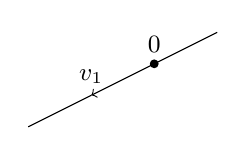
\begin{tikzpicture}[scale = 0.8]
	\draw[->] (0,0) -- (-2,-1) node at (-2,-0.7) {\small $v_1$};
	\draw (-2,-1) -- (-3,-1.5);
	\fill (-1,-0.5) circle (2pt) node at (-1,-0.2) {\small  $0$};	
	\end{tikzpicture}
	\end{center}
	\item For $n=3$, $v_1,v_2,v_3$ are linearly dependent iff $x_1v_1 + x_2v_2 + x_3v_3 =  0$ and one of the coefficients $ \neq 0$, say $x_1 \neq 0$. Then $v_1 = -\frac{x_2}{x_1}v_2 - \frac{x_3}{x_1}v_3$. In $\R^3$, $v_1$ lies in the plane through $0, v_2,v_3$: 
		\begin{center}
	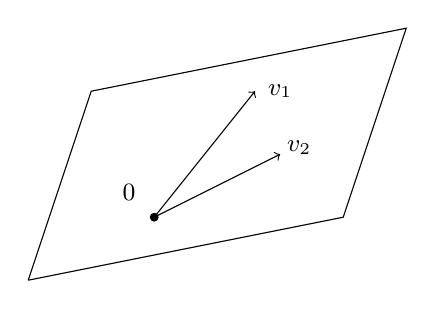
\begin{tikzpicture}[scale =0.8]
	\draw[<-] (0,0) -- (-2,-1) node at (0,1) {\small $v_1$};
	\draw[->] (-2,-1) -- (-0.4,1) node at (0.3,0.1) {\small  $v_2$};
	\fill (-2,-1) circle (2pt) node at (-2.4,-0.6) {\small $0$};	
	\draw (-4,-2) -- (1,-1) -- (2,2) -- (-3,1) -- (-4,-2);
	\end{tikzpicture}
	\end{center}
	
	Conclusion: $v_1,v_2,v_3 \iR^3$ are linearly dependent iff they belong to a plane through $0$. 
\end{enumerate}
\end{examples}\vsp

\begin{lemma}
(i) Let $v_1,v_2\iR^2$. Define a $2\times 2$ matrix $B$ such that $v_1,v_2$ are the columns of $B$: 
\[
  B = \begin{pmatrix}
 | & | \\ v_1 & v_2 \\ | & |	
 \end{pmatrix}
\]
Then $\det(B) = 0$ iff $v_1$ and $v_2$ are linearly dependent. 

(ii) Let $v_1,v_2,v_3\iR^3$ and define a $3 \times 3$ matrix $B$ so that $v_1,v_2,v_3$ are the columns of $B$. Then $\det(B) = 0$ iff $v_1,v_2,v_3$ are linearly dependent. 
\end{lemma}

\begin{proof}[Proof of (ii)]
Note that 
\begin{align*}
  B\begin{pmatrix}
x_1 \\ x_2 \\ x_3	
\end{pmatrix} &= \begin{pmatrix}
 | & | & | \\ v_1 & v_2 & v_3 \\ | & | & |	
 \end{pmatrix}
\begin{pmatrix}
x_1 \\ x_2 \\ x_3	
\end{pmatrix}\\
&= x_1v_1 + x_2v_2 + x_3v_3
\end{align*}
We know that $\det(B) = 0 \iff Bx = 0$ has a non-zero solution, where $x =(x_1,x_2,x_3)^t \iff x_1v_1 + x_2v_2 + x_3v_3 = 0$ where some $x_1 \neq 0 \iff v_1,v_2,v_3$ are linearly dependent. 
\end{proof}\vsp

\begin{theorem}
Let $A$ be a square matrix ($3 \times 3$ case) with eigenvectors $v_1,v_2,v_3$ with eigenvalues $\lambda_1,\lambda_2,\lambda_3$ respectively. Define 
\[
  D = \mathrm{diag}(\lambda_1,\lambda_2,\lambda_3) = \begin{pmatrix}
 \lambda_1 & 0 & 0\\ 0 & \lambda_2 & 0\\ 0 & 0 & \lambda_3	
 \end{pmatrix}
\]
$P$ as a matrix with columns $v_1,v_2,v_3$. 

a) Then $AP = PD$

b) If $v_1,v_2,v_3$ are linearly independent, then $P^{-1}$ exists and $A = PDP^{-1}$
\end{theorem}\vsp

\emph{Remark.} This is a theorem about the diagonalisation of matrices

\begin{proof}
	a) What is $AP$? The $i$-th column of $AP$ is $c_i(AP) = Ac_i(P) $ (lecture 8) 
	\[
  c_i(AP) = Ac_i(P) = Av_i = \lambda_iv_i
\]
What is $PD$?
\begin{align*}
  PD &= \begin{pmatrix}
 | & | & | \\ v_1 & v_2 & v_3 \\ | & | & |	
 \end{pmatrix}\begin{pmatrix}
 \lambda_1 & 0 & 0\\ 0 & \lambda_2 & 0\\ 0 & 0 & \lambda_3	
 \end{pmatrix}\\
 &= \begin{pmatrix}
 | & | & | \\ \lambda_1v_1 & \lambda_2v_2 & \lambda_3v_3 \\ | & | & |	
 \end{pmatrix}
\end{align*}
Hence $AP = PD$.

b) By Lemma 7.2, $P^{-1}$ exists iff $v_1,v_2,v_3$ are linearly independent.
\end{proof}\vsp

\begin{definition}
\lecturemarker{15}{14/11}
Two square matrices $A$ and $B$ are called \emph{equivalent} if there exists an invertible matrix $P$ such that $A = PBP^{-1}$. 
\end{definition}

\emph{Exercise:} Check that this is indeed an equivalence relation.\\

\begin{definition}
A square matrix $A$ is \emph{diagonalisable} if $A$ is equivalent to a diagonal matrix, i.e. $\exists$ an invertible matrix $P$ such that $A = PDP^{-1}$, where $D$ is diagonal. 
\end{definition}\vsp

\begin{proposition}~\\[.1cm]
(i) If $A$ is a diagonalisable $2 \times 2$ matrix, then $A$ has two linearly independent eigenvectors (not multiples of each other)

(ii) If $A$ is a diagonalisable $3 \times 3$ matrix, then $A$ has three linearly independent eigenvectors.  	
\end{proposition}

\emph{Remark.} This is in fact an ``if and only if" statement (as it follows from Theorem 7.3)

\begin{proof}[Proof of (ii)]
$A = PDP^{-1}$ where $D = \mathrm{diag}(\lambda_1,\lambda_2,\lambda_3)$. Then $AP = PD$. Next, consider the columns of $P$ as three vectors, call them $v_1,v_2,v_3$. 
\begin{align*}
  PD &= \begin{pmatrix}
 | & | & | \\ v_1 & v_2 & v_3 \\ | & | & |	
 \end{pmatrix}\begin{pmatrix}
 \lambda_1 & 0 & 0\\ 0 & \lambda_2 & 0\\ 0 & 0 & \lambda_3	
 \end{pmatrix}\\
 &= 
 \begin{pmatrix}
 \lambda_1p_{11} & \lambda_2p_{12} & \lambda_3p_{13}\\
 \lambda_1p_{21} & \lambda_2p_{22} & \lambda_3p_{23}\\
 \lambda_1p_{31} & \lambda_2p_{32} & \lambda_3p_{33}	
 \end{pmatrix}\\
 &= \begin{pmatrix}
  | & | & | \\ \lambda_1v_1 & \lambda_2v_2 & \lambda_3v_3 \\ | & | & |		
 \end{pmatrix}
\end{align*}
Now $AP = PD \implies c_i(PD) = \lambda_iv_i \implies c_i(AP) = Ac_i(P) = Av_i$ for $i = 1,2,3$. Hence $v_i$ is an eigenvector of $A$ with eigenvalue $\lambda_i$. 

\textbf{Claim:} $v_1,v_2,v_3$ are linearly independent. In fact, Lemma 7.2 says $P^{-1}$ exists iff they are linearly independent. Since $P^{-1}$ exists, we're done.
\end{proof}\vsp


\begin{corollary}~\\[-.2cm]
\begin{enumerate}
\item All matrices that are equivalent to 
\[
  J_\lambda = \begin{pmatrix}
 \lambda & 1 & 0\\ 0 & \lambda & 1\\\ 0 & 0 & \lambda 	
 \end{pmatrix}
\]
for $\lambda \iR$, are non-diagonalisable.
\item All matrices equivalent to 
\[
  J_{\lambda_1\mu} = \begin{pmatrix}
 \lambda & 1 & 0\\ 0 & \lambda & 0 \\ 0 & 0 & \mu 	
 \end{pmatrix}
 \]
 for any $\lambda_1,\mu \iR$ are also non-diagonalisable.
\end{enumerate}
\end{corollary}

\emph{Remark.} These are in fact all the non-diagonalisable matrices.

\begin{proof}(i) For contradiction, suppose that $A = BJ_\lambda B^{-1}$ (for some invertible matrix $B$) is diagonalisable. Then $A = PDP^{-1}$, so $BJ_\lambda B^{-1} = PDP^{-1} \implies J_{\lambda} = B^{-1}PDP^{-1}B$. We know that $(B^{-1}P)^{-1} = P^{-1}(B^{-1})^{-1} = P^{-1}B$. Therefore $J_{\lambda} = (B^{-1}P)D(B^{-1}P)^{-1}$. 

So $J_\lambda$ is diagonalisable and by Prop 7.4, $J_\lambda$ must have three linearly independent eigenvectors. Let's find them:

\[
  tI - J_\lambda = \begin{pmatrix}
 t - \lambda & -1 & 0 \\ 0 & t-\lambda & -1 \\ 0 & 0& t-\lambda 	
 \end{pmatrix}
\]
\[
  \det(tI-J_\lambda) = (t-\lambda)^3
\]
Hence $\lambda$ is the only eigenvalue of $J_\lambda$. The corresponding eigenvectors satisfy $(\lambda I - J_\lambda)v = 0$, i.e. 
\[
  \begin{pmatrix}
  0 & -1 & 0\\ 0 & 0 & -1 \\ 0 & 0 & 0	
  \end{pmatrix}\begin{pmatrix}
x_1 \\ x_2 \\ x_3	
\end{pmatrix} = \begin{pmatrix}
 0 \\ 0\\ 0	
 \end{pmatrix}
\]
$\implies x_2 = x_3 = 0, x_1 = a \iR$. Hence we conclude \[v = \begin{pmatrix}
 1 \\ 0 \\ 0	
 \end{pmatrix}\] up to scalar multiples is the only eigenvector. So there are not three linearly independent eigenvectors, a contradiction. Thus $A = BJ_\lambda B^{-1}$ is not a diagonalisable matrix.
\end{proof}

\emph{Exercise:} Prove (ii) similarly.\\


\begin{examples}
(1) Let 
\[
  A = \begin{pmatrix}
 3 & 2 \\ 2 & 0	
 \end{pmatrix}
\]
In lecture 13, we found this has eigenvalues $\lambda_1 = 4,\, \lambda_2 -1$. The corresponding eigenvectors are 
\[
  v_1 = \begin{pmatrix}
 2 \\ 1	
 \end{pmatrix} \quad v_2 = \begin{pmatrix}
 1 & -2	
 \end{pmatrix}
\]
So $A = PDP^{-1}$ where 
\[
  D = \begin{pmatrix}
  4 & 0 \\ 0 & -1
 \end{pmatrix}\quad 
 P = \begin{pmatrix}
 2 & 1 \\ -1 & -2	
 \end{pmatrix}
\]
So $A^2 = (PDP^{-1})(PDP^{-1}) = PD^2P^{-1}$. (By induction $A^n = PD^nP^{-1}$ since $PP^{-1} = I$). 
\[
  P^{-1} = \frac{1}{-5} \begin{pmatrix}
 -2 & -1\\ -1 & 2	
 \end{pmatrix}
 = \frac{1}{5}\begin{pmatrix}
2 & 1 \\ 1 & -2	
\end{pmatrix}
\]
Therefore, $A^n = PD^nP^{-1}$
\begin{align*}
  \implies A^n &= \frac{1}{5}\begin{pmatrix}
2 & 1\\ 1& -2	
\end{pmatrix}\begin{pmatrix}
4^n & 0 \\ 0 & (-1)^n	
\end{pmatrix}\begin{pmatrix}
2 & 1 \\ 1 & -2	
\end{pmatrix}\\[.2cm]
&= \frac{1}{5}\begin{pmatrix}
2\cdot 4^n & (-1)^n \\ 4^n & -2(-1)^n	
\end{pmatrix}\begin{pmatrix}
2 & 1\\ 1 & -2	
\end{pmatrix}\\[.2cm]
&= \frac{1}{5}\begin{pmatrix}
4^{n=1} + (-1)^n & 2\cdot 4^n - 2(-1)^n\\
2\cdot 4^n-2(-1)^n & 4^n+4(-1)^n	
\end{pmatrix}
\end{align*}

(2) How do we find a $2 \times 2$ matrix $B$ such that $B^3 = A$?

Idea: Take any $2 \times 2$ matrix $C$ such that $C^3 = D$ e.g. 
\[
  C = \begin{pmatrix}
 4\frac{1}{3} & 0 \\ 0 & (-1)	
 \end{pmatrix}
\]
Then $B = PCP^{-1}$ works. Indeed $B^3 = PC^3P^{-1} = PDP^{-1} = A$.\\

(3) Fibonacci Sequence
\[
  0,1,1,2,3,5,8,13,21,35,55,\dots
\]
Formally defined as $f_{n+1} = f_n + f_{n-1} \quad f_0 = 0,\, f_1 = 1$. 

Let 
\[
  A = \begin{pmatrix}
 1 & 1 \\ 1 & 0	
 \end{pmatrix}
\]
Notice that 
\[
  \begin{pmatrix}
  f_{n+1}\\ f_n	
  \end{pmatrix}
  = A\begin{pmatrix}
f_n \\ f_{n-1}	
\end{pmatrix}
\]
Since $f_{n+1} = f_n + f_{n-1}$... 
\begin{align*}
  \begin{pmatrix}
  f_{n+1}\\ f_n 	
  \end{pmatrix} &= 
  A\begin{pmatrix}
	f_n \\ f_{n-1}
\end{pmatrix}\\
&= A^2 \begin{pmatrix}
 f_{n-1} \\ f_{n-2}	
 \end{pmatrix}\\
 &= \dots\\
 &= A^n\begin{pmatrix}
f_1 \\ f_0	
\end{pmatrix}\\
&= A^n \begin{pmatrix}
	1 \\ 0
\end{pmatrix}
\end{align*}
We now know how to find $A^n$, and this gives a formula for $f_n$. \\

(4) Is 
\[
  A = \begin{pmatrix}
  1& 0 & 0\\ -1 & 2 & 0\\ 1 & -1 & 1	
 \end{pmatrix}
\]
diagonalisable? 

The characteristic polynomial is $(t-1)^2(t-2)$, so $\lambda_1 = 2,\, \lambda_2 = 1$. We find
\[
  v_1 = \begin{pmatrix}
 0 \\ 1 \\ -1	
 \end{pmatrix}
\]
is an eigenvector with eigenvalue $\lambda_1$. 

We can find two non-proportional eigenvectors for $\lambda_1 = 1$. Then three eigenvectors are linearly independent. So $A$ is diagonalisable. [So sometimes double root $\implies$ three eigenvectors and is still diagonalisable.] 

\end{examples}
\vspace*{1cm}




\begin{center}

\includegraphics[width=9cm]{cartoon2.png}	
\end{center}




\sektion{Conics and Quadrics}


Back to $2$-dim geometry, we work in $\R^2$. \lecturemarker{16}{18/11}

Lines are given by linear equations
\[
  ax_1 + bx_2 + c = 0
\]
(polynomial equations in $x_1,x_2$ of degree $2$)\\


\begin{definition}
A conic is a curve in $\R^2$ that can be given by a quadratic equation, i.e. a polynomial equation in $x_1,x_2$ of degree $2$.
\[
  ax_1^2 + bx_1x_2 + cx_2^2 + dx_1 + cx_2 + f = 0
\]
\end{definition}

e.g. $x_1^2 + x^2 = r_2$ gives a circle. Also $(ax_1 + bx_2 + c)(a'x_1 + b'x_2 + c') = 0$ is the set of solutions is the union of two lines. 

\subsektion{Standard Forms of Conics}

\textbf{Non-degenerate conics:}

For $a \neq 0, b \neq 0 \iR$ we have

(1) An ellipse
\[
  \frac{x_1^2}{a^2} + \frac{x_2^2}{b^2} = 1\]


\begin{center}
\begin{tikzpicture}
  \draw[->] (-3,0) -- (3,0) node[right] {$x_1$};
  \draw[->] (0,-1.5) -- (0,1.5) node[above] {$x_2$};
 \draw[scale=0.55,domain=-3.141:3.141,smooth,variable=\t] plot ({2*sin(\t r)},{1.5*cos(\t r)});
\end{tikzpicture}
\end{center}




(2) A hyperbola
\[
  \frac{x_1^2}{a^2} - \frac{x_2^2}{b^2} = 1 
\]


\begin{center}
\begin{tikzpicture}
  \draw[->] (-3,0) -- (3,0) node[right] {$x_1$};
  \draw[->] (0,-1.5) -- (0,1.5) node[above] {$x_2$};
 \draw[scale=0.55,domain=-1:1,smooth,variable=\t] plot ({2*sec(\t r)},{1.5*tan(\t r)});
  \draw[scale=0.55,domain=-1:1,smooth,variable=\t] plot ({-2*sec(\t r)},{1.5*tan(\t r)}); 
  \draw [dashed] (-1.5,-1.5) -- (1.5,1.5);
    \draw [dashed] (1.5,-1.5) -- (-1.5,1.5);
\end{tikzpicture}
\end{center}


(3) An imaginary ellipse
\[
-\frac{x_1^2}{a^2} - \frac{x_2^2}{b^2} = 1
\]
This defines an empty set (there are no solutions). 



(4) A parabola
\[
x_2 = ax_1^2 + b
\]


\begin{center}
\begin{tikzpicture}
  \draw[->] (-3,0) -- (3,0) node[right] {$x_1$};
  \draw[->] (0,-1) -- (0,1.5) node[above] {$x_2$};
 \draw[scale=0.8,domain=-1:1,smooth,variable=\t] plot ({\t},{abs(2*\t^2) + 0.5});
 \fill (0,0.4) circle (1pt);
 \node at (0.4,0.4) {$b$};
 \end{tikzpicture}
\end{center}


\textbf{Degenerate conics:}


(5) Two lines with a common point
\[
  \frac{x_1^2}{a^2} - \frac{x_2^2}{b^2} = 0  \implies  \left(\frac{x_1}{a} - \frac{x_2}{b}\right)
  \left(\frac{x_1}{a} + \frac{x_2}{b}\right) 
  = 0\]

\begin{center}
\begin{tikzpicture}[scale =0.8]
  \draw[->] (-3,0) -- (3,0) node[right] {$x_1$};
  \draw[->] (0,-1.5) -- (0,1.5) node[above] {$x_2$};
  \draw  (-1.5,-1.5) -- (1.5,1.5);
    \draw (1.5,-1.5) -- (-1.5,1.5);
\end{tikzpicture}
\end{center}


(6) $x_1^2 = 0$, a double line. 



(7) A pair of two conjugate complex lines meeting in a real point
\[
  \frac{x_1^2}{a^2} + \frac{x_2^2}{b^2} = 0 \implies \left(\frac{x_1}{a} - i\frac{x_2}{b}\right)
  \left(\frac{x_1}{a} + i\frac{x_2}{b}\right) 
  = 0
\]
The set of real solutions is one point $(0,0)$. 

(8) Two parallel lines
\[
  \frac{x_1^2}{a^2} = 1 \quad (\frac{x_1}{a} = \pm 1)
\]


\begin{center}
\begin{tikzpicture}
  \draw[->] (-3,0) -- (3,0) node[right] {$x_1$};
  \draw[->] (0,-1.5) -- (0,1.5) node[above] {$x_2$};
  \draw  (-1.5,-1.5) -- (-1.5,1.5);
    \draw (1.5,1.5) -- (1.5,-1.5);
\end{tikzpicture}
\end{center}


(9) A pair of parallel complex conjugate lines
\[
  \frac{x_1^2}{a^2} = 1
\]
There are no real solutions. $\frac{x_1}{a} = \pm i$.

\subsektion{Reducing with Trigonometry}

\textbf{Our aim:} To use translations and rotations in $\R^2$ to reduce any conic to one of these standard types. 


\emph{Why conics?} These are all slices of the cone $x^2 + y^2 = z^2$:
\begin{center}
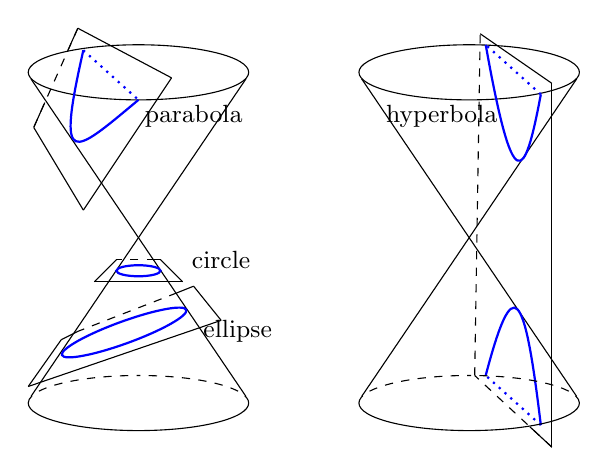
\begin{tikzpicture}[scale = 0.7]
\draw[black] (-3,3) ellipse (2 and 0.5);
\draw[black] (3,3) ellipse (2 and 0.5);
\draw[] (-4.95,2.88) -- (-1.05,-2.88);
\draw[] (-4.95,-2.88) -- (-1.05,2.88);
\draw[] (4.95,2.88) -- (1.05,-2.88);
\draw[] (4.95,-2.88) -- (1.05,2.88);

\draw[blue, thick] (-3,-0.6) ellipse (0.4 and 0.1);
\draw[] (-3.8,-0.8) -- (-2.2,-0.8);
\draw[] (-3.8,-0.8) -- (-3.4,-0.4);
\draw[] (-2.2,-0.8) -- (-2.6,-0.4);
\draw[] (-3.4,-0.4) -- (-3.3,-0.4);
\draw[] (-2.6,-0.4) -- (-2.7,-0.4);
\draw[dashed] (-2.7,-0.4) -- (-3.3,-0.4);
\node[] at (-1.5,-0.4) {\small circle};

\draw[rotate around={20:(-3.26,-1.72)}, blue, thick] (-3.26,-1.72) ellipse (1.2 and 0.2);
\draw[] (-5,-2.7) -- (-1.5,-1.5);
\draw[] (-5,-2.7) -- (-4.4,-1.85);
\draw[] (-4.4,-1.85) -- (-4.1,-1.7);
\draw[] (-1.5,-1.5) -- (-2,-0.88);
\draw[] (-2,-0.88) -- (-2.3,-1);
\draw[dashed] (-2.3,-1) -- (-4.1,-1.7);
\node[] at (-1.2,-1.7) {\small ellipse};

\draw[blue, thick] (-4,3.4) .. controls (-4.5,1.2) and (-4.2,1.5) .. (-3,2.5);
\draw[dotted, blue, thick] (-4,3.4) -- (-3,2.5);
\draw[] (-2.4,2.9) -- (-4,0.5);
\draw[] (-2.4,2.9) -- (-4.1,3.8) coordinate (A);
\draw[] (-4,0.5) -- (-4.9,2) coordinate (B);
\draw[dashed] (A) -- (B);
\draw[] (A) -- (-4.28,3.4);
\draw[] (B) -- (-4.7,2.45);
\node[] at (-2,2.2) {\small parabola};

\draw[] (4.5,-3.8) coordinate (A) -- (4.5,2.8) coordinate (B);
\draw[dashed] (A) -- (3.1,-2.5) coordinate (C);
\draw[] (B) -- (3.2,3.7) coordinate (D);
\draw[dashed] (C) -- (D);
\draw[blue, thick] (4.3,-3.4) coordinate (E) .. controls (4,-0.9) and (3.8,-0.6) .. (3.3,-2.5) coordinate (F);
\draw[dotted, blue, thick] (E) -- (F); 
\draw[blue, thick] (4.3,2.6) coordinate (G) .. controls (4,1) and (3.8,0.7) .. (3.3,3.5) coordinate (H);
\draw[dotted, blue, thick] (G) -- (H); 
\draw[] (A) -- (4.1,-3.43);
\node[] at (2.5,2.2) {\small hyperbola};

\pgfpathmoveto{\pgfpoint{-1cm}{-3cm}}
\pgfpatharcto{2cm}{0.5cm}{0}{0}{0}{\pgfpoint{-3cm}{-3.5cm}}
\pgfpathmoveto{\pgfpoint{-5cm}{-3cm}}
\pgfpatharcto{2cm}{0.5cm}{0}{0}{-1}{\pgfpoint{-3cm}{-3.5cm}}
\pgfstroke

\pgfsetdash{{3pt}{3pt}}{0pt}
\pgfpathmoveto{\pgfpoint{-1cm}{-3cm}}
\pgfpatharcto{2cm}{0.5cm}{0}{0}{-1}{\pgfpoint{-3cm}{-2.5cm}}
\pgfpathmoveto{\pgfpoint{-5cm}{-3cm}}
\pgfpatharcto{2cm}{0.5cm}{0}{0}{0}{\pgfpoint{-3cm}{-2.5cm}}
\pgfstroke

\pgfsetdash{{3pt}{0pt}}{0pt}
\pgfpathmoveto{\pgfpoint{1cm}{-3cm}}
\pgfpatharcto{2cm}{0.5cm}{0}{0}{-1}{\pgfpoint{3cm}{-3.5cm}}
\pgfpathmoveto{\pgfpoint{5cm}{-3cm}}
\pgfpatharcto{2cm}{0.5cm}{0}{0}{0}{\pgfpoint{3cm}{-3.5cm}}
\pgfstroke

\pgfsetdash{{3pt}{3pt}}{0pt}
\pgfpathmoveto{\pgfpoint{1cm}{-3cm}}
\pgfpatharcto{2cm}{0.5cm}{0}{0}{0}{\pgfpoint{3cm}{-2.5cm}}
\pgfpathmoveto{\pgfpoint{5cm}{-3cm}}
\pgfpatharcto{2cm}{0.5cm}{0}{0}{-1}{\pgfpoint{3cm}{-2.5cm}}
\pgfstroke
\end{tikzpicture}
\end{center}

\begin{enumerate}
\item $z = $ constant $ \implies$ a circle / ellipse.
\item $z = y + 1$ into equation $\implies x^2 = 2y + 1$, a parabola.	
\item $y=1$ (vertical plane) $\implies$ a hyperbola.
\item $z = 0,\,x^2+y^2$: two conjugate lines with a common real point. 
\item $y = 0,\, x^2 = z^2$: two real lines.
\end{enumerate}\vsp



\textbf{Translations in $\R^2$:}

\begin{center}
\begin{tikzpicture}
\draw[->] (-3,0) -- (3,0) node at (3,-0.3) {$x_1$};
\draw[->] (0,-2) -- (0,2) node at (-0.3,2) {$x_2$};
\begin{scope}[shift  ={(2,1)}]
\draw[dashed,->] (-5,0) -- (1,0) node at (1,-0.3) {$y_1$};
\draw[dashed,->] (0,-3) -- (0,1) node at (-0.3,1) {$y_2$};	
\end{scope}

\end{tikzpicture}
\end{center}
Moving the co-ordinates by $(d_1,d_2)$ has the effect that
\begin{align*}
  x_1 &= y_1 + d_1\\
  x_2 &= y_2 + d_2
\end{align*}

\textbf{Rotations in $\R^2$}

Recall that rotating coordinate $P = (p_1,p_2)$ to $Q = (q_1,q_2)$ by $\varphi$ through $O$ is: 
\[
  \begin{pmatrix}
  q_1 \\ q_2	
  \end{pmatrix} = \begin{pmatrix}
 \cos\varphi & -\sin\varphi \\
 \sin\varphi & \cos\varphi 	
 \end{pmatrix}\begin{pmatrix}
	p_1 \\ p_2	
	\end{pmatrix}
\]

\emph{What is the effect of rotation on coordinates?} 

Rotating the $(x_1,x_2)$ coordinate system by $\varphi$:

\begin{center}
\begin{tikzpicture}
\draw[->] (-3,0) -- (3,0) node at (3,-0.3) {$x_1$};
\draw[->] (0,-2) -- (0,2) node at (-0.3,2) {$x_2$};
\draw[rotate = 20,->,dashed] (-3,0) -- (3,0) node at (3,-0.3) {$y_1$};
\draw[rotate = 20,->,dashed] (0,-2) -- (0,2) node at (-0.3,2) {$y_2$};
\draw [rotate= 10,->] (0,0) -- (2,1) node [above] {$P$}; 
\draw [rotate = 30, ->, dashed] (0,0) -- (2,1) node [above] {$Q$}; 
\node at (1,0.2) {$\varphi$};	
\node at (0.8,0.8) {$\varphi$};	
\end{tikzpicture}
\end{center}


The $y_1,y_2$ coordinates of $Q$ are simply $p_1$ and $p_2$. Therefore, the new coordinates $y_1,y_2$ and the old coordinates $x_1,x_2$ are related as follows:
\[
  \begin{pmatrix}
  x_1 \\ x_2	
  \end{pmatrix} = \begin{pmatrix}
 \cos\varphi & -\sin\varphi\\
 \sin\varphi & \cos\varphi 	
 \end{pmatrix} \begin{pmatrix}
 y_1 \\ y_2	
 \end{pmatrix}
 \]
 
 
Let's write quadratic equations in matrix form. Recall that $A^t$ denotes the transpose of $A$, i.e. the matrix whose $i-j$ entry is the $j-i$ entry of $A$. \\

\begin{definition}
A square matrix is called \emph{symmetric} if $A^t = A$.
\end{definition}

e.g. 
\[
  \begin{pmatrix}
  a & b \\ b & a	
  \end{pmatrix},\quad 
  \begin{pmatrix}
  a & b & c \\ b & d & e \\ c & e & f	
  \end{pmatrix}
\]

Recall that we proved that $(AB)^t = B^t\cdot A^t$ and  $(A+B)^t = A^t + B^t$. 
Consider \[
    A = \begin{pmatrix}
  	a & \frac{1}{2}b \\ \frac{1}{2}b & c
  \end{pmatrix}
\]
\begin{align*}
  (x_1,x_2)\begin{pmatrix}
  	a & \frac{1}{2}b \\ \frac{1}{2}b & c
  \end{pmatrix}\begin{pmatrix}
	x_1 \\ x_2	
	\end{pmatrix}
	&= (x_1,x_2)\begin{pmatrix}
ax_1 + \frac{1}{2}bx_2 \\
\frac{1}{2}bx_1 + cx_2	
\end{pmatrix}\\[.2cm]
&= x_1(ax_1 + \textstyle{\frac{1}{2}}bx_2) + x_2(\textstyle{\frac{1}{2}}bx_1 + cx_2)\\[.2cm]
&= ax_1^2 + bx_1x_2 + cx_2^2
\end{align*}
\[
  (x_1,x_2) \begin{pmatrix}
 d \\ e	
 \end{pmatrix} = dx_1 + ex_2 = (d,e) \begin{pmatrix}
 x_1 \\ x_2	
 \end{pmatrix}
\]


Therefore we can write $ax_1^2 + bx_1x_2 + cx_2^2 + dx_1 + ex_2 + f$ as 
\[
  x^tAx + (d,e)x + f
\]
where $x = \begin{pmatrix}
 x_1 \\ x_2	
 \end{pmatrix}$, $x^t = (x_1,x_2)$.\\
 
 
\begin{theorem}
 Using a \lecturemarker{17}{20/11} rotation and then translation we can always reduce any quadratic equation to standard form. 	
\end{theorem}

Low level proof - Idea: Get rid of the $x_1x_2$ terms using a rotation. If we can do that, then for some new coefficients $a',c',d',e',f'$ we obtain:
\[
  a'y_1^2 + c'y_2^2 + d'y_1 + e'y_2 + f'
\]
we complete the squares and reduce this equation to 
\[
  a''z_1^2 + c''z_2^2 + f''
\]
or (when $c' = 0$)
\[
  a''z_1^2 + e''z_2 + f'' 
\]

\begin{proof}
Rotate through $\varphi$, then 
\[
  \begin{pmatrix}
  x_1 \\ x_2	
  \end{pmatrix} = R_\phi\begin{pmatrix}
y_1 \\ y_2	
\end{pmatrix} = \begin{pmatrix}
	\cos\varphi & -\sin\varphi\\ \sin\varphi & \cos\varphi 
\end{pmatrix}\begin{pmatrix}
y_1 \\ y_2	
\end{pmatrix}
\]
\[
  \implies x^tAx = (R\varphi y)^tA(R_\varphi y) = y^tR_\varphi^t AR_\varphi y\\
\]

We want the matrix $R_\varphi^t AR_\varphi y$ to be diagonal (then $y_1y_2$ terms disappears) 

\begin{align*}
  R_\varphi^tAR_\varphi &= \begin{pmatrix}
 \cos\varphi & \sin\varphi \\ -\sin\varphi & \cos\varphi 	
 \end{pmatrix}\begin{pmatrix}
a & \frac{1}{2}b \\ \frac{1}{2}b & c 	
\end{pmatrix}R_\varphi\\
&= 
\begin{pmatrix}
a \cos\varphi + \frac{1}{2}b\sin\varphi 	& \frac{1}{2}b\cos\varphi + c\sin\varphi\\
-a\sin\varphi + \frac{1}{2}b\cos\varphi & -\frac{1}{2}b\sin\varphi + c\cos\varphi 
\end{pmatrix}\begin{pmatrix}
\cos\varphi & -\sin\varphi\\
\sin\varphi & \cos\varphi 	
\end{pmatrix}
\end{align*}

We need to know the non-diagonal terms. The $12$ entry is 
\begin{align*}
 &-a\sin\varphi\cos\varphi - \frac{1}{2}b\sin^2\varphi + \frac{1}{2}b\cos^2\varphi + c\sin\varphi\cos\varphi\\
 &= -\frac{1}{2}a\sin2\varphi + \frac{1}{2}b\cos2\varphi + \frac{1}{2}c\sin2\varphi\\
 &= \frac{1}{2}(b\cos2\varphi - (a-c)\sin2\varphi)
\end{align*}

If $a \neq c$, then take $\varphi$ such that $\tan2\varphi = \frac{b}{a-c}$ (then this term is $0$). 

If $a = c$, take $\varphi = \frac{\pi}{4}$ (again, $0$). 

After this rotation, $x = R_\varphi y$, we accomplished the first step. Then we obtain the equation
\[
  a'y_1^2 + c'y_2^2 + d'y_1 + e'y_2 + f
\]
If $a'\neq 0$, $c' \neq 0$, we can complete the squares and reduce this to 
\[
  a'z_1^2 + c'z_2^2 + f''
\]
Then
\begin{align*}
  y_1 &= z_1 + \alpha_1\\
  y_2 &= z_2 + \alpha_2
\end{align*}
This is exactly a translation by $(\alpha_1,\alpha_2)$. If $a'\neq 0$, but $c' = 0$, we complete the square for $y_1$ and do nothing for $y_2$. Then reduce to $a'z_1^2 + e''z_2 + f''$. We get a parabola or a degenerate conic. 
\end{proof}\vsp


\begin{example} Reduce to standard form 
\[
  5x_1^2 + 4x_1x_2 + 2x_2^2 + x_1 + x_2 - 1 = 0
\]


\textsc{Step 1:} 
\[
  A = \begin{pmatrix}
	5 & 2 \\ 2 & 2 	
 \end{pmatrix}
\]
Use $R_\varphi = \tan2\varphi =  \frac{b}{a-c} = \frac{4}{3}$. We can calculate $\sin\varphi = \frac{2}{\sqrt{5}}$, $\cos\varphi = \frac{1}{\sqrt{2}}$. 
\[
  \begin{pmatrix}
  x_1 \\ x_2	
  \end{pmatrix} 
  = \frac{1}{\sqrt{5}}
  \begin{pmatrix}
  1 & 2 \\ -2 & 1	
  \end{pmatrix}\begin{pmatrix}
 y_1\\ y_2	
\end{pmatrix}
\]
Substitute into equations and obtain 
\[
  5x_1^2 + 4x_1x_2 + 2x_2^2 = y_1^2 + 6y_2^2
\]
The new equation is 
\begin{align*}
&y_1^2 + 6y_2^2 - \frac{1}{\sqrt{5}}y_1 + \frac{3}{\sqrt{5}}y_2 - 1 = 0\\
&= (y_1 - \frac{1}{2\sqrt{5}})^2 + 6(y_2 + \frac{1}{4\sqrt{5}})^2 - \frac{9}{8}\\
&= z_1^2 + 6z_2^2 - \frac{9}{8}  
\end{align*}
so this is an ellipse.
\end{example}\vsp 

\subsektion{Reducing with Eigenvectors}

There is a trigonometry-free method!

Note for any rotation matrix, we have $R_\varphi^t = R_\varphi^{-1}$. Indeed 
\begin{align*}
  R_\varphi &= \begin{pmatrix}
 \cos\varphi & -\sin\varphi\\
 \sin\varphi & \cos\varphi 	
 \end{pmatrix}
\end{align*}
\begin{align*}
  R_\varphi^t &= \begin{pmatrix}
 \cos\varphi & \sin\varphi\\
 -\sin\varphi & \cos\varphi 	
 \end{pmatrix}
\end{align*}
and 
\[
  \begin{pmatrix}
  \cos\varphi & \sin\varphi\\
  -\sin\varphi & \cos\varphi 	
  \end{pmatrix}\begin{pmatrix}
\cos\varphi & -\sin\varphi \\
\sin\varphi & \cos\varphi 	
\end{pmatrix}= \begin{pmatrix}
 1 & 0 \\ 0 & 1	
 \end{pmatrix}
\]
\vsp

\begin{definition}
Let $P$ be a square matrix of the size $n \times n$. Then $P$ is called \emph{orthogonal} if $P^t\cdot P = I$. (In otherwords, $P^{-1}$ exists and equals $P^t$)	
\end{definition}

Since the rows of $P^t$ are precisely the columns of $P$, $P^tP = I$ is equivalent to the following property:
\[
  (c_i(P)\cdot c_j(P)) = \begin{cases}
 1,\, i = j\\
 0,\, i\neq j	
 \end{cases}
\]
In sheet 6, there is an exercise that says a $2\times 2$ matrix is orthogonal $\iff$ $P$ is a rotation matrix or a reflection matrix; depending on whether $\det(P) = 1$ or $\det(P) = -1$. Note  $R_\varphi^tAR_\varphi = R_\varphi^{-1}AR_\varphi$. In the proof of Theorem 8.1, we watned $R_\varphi^tAR_\varphi = R_\varphi^{-1}AR_\varphi$ to be diagonal. 

New idea: Use diagonalisation, that 
\[
  P = \begin{pmatrix}
 | & | \\
 v_1 & v_2\\ 
 | & |	
 \end{pmatrix}
\]
where $v_1,v_2$ are the eigenvectors of $A$.

\emph{Why do $v_1,v_2$ exist? Why is $P$ a rotation matrix? }




\begin{theorem}
Let $A$ be any real symmetric $2 \times 2$ matrix 
\[
  A = \begin{pmatrix}
 a & \frac{1}{2}b\\ \frac{1}{2}b & c	
 \end{pmatrix}\quad \mbox{such that $A \neq \begin{pmatrix}
 \alpha & 0 \\ 0 & \alpha	
 \end{pmatrix}$ for some $\alpha \iR$. }
\]
Then $A$ has the following properties: 
\begin{enumerate}
\item $A$ has two different real eigenvalues $\lambda_1, \lambda_2\,\,\lambda_1 \neq \lambda_2$
\item 	If $v_1$ is an eigenvector, with eigenvalue $\lambda_1$ and $v_2$ is an eigenvector with eigenvalue $\lambda_2$. Then $v_1\cdot v_2 = 0$ (i.e. $v_1,v_2$ are perpendicular)
\item Up to swapping $v_1$ and $v_2$ and multiplying $v_1,v_2$ by a scalar, so that $||v_1|| = ||v_2|| = 1$, the matrix 
\[
  P = \begin{pmatrix}
 | & | \\
 v_1 & v_2\\ 
 | & |	
 \end{pmatrix}
\]
is a rotation matrix.
\end{enumerate}
\end{theorem}


\begin{proof}
(i)	
\begin{align*}
  \det\begin{pmatrix}
 t-a & -\frac{1}{2}b \\ -\frac{1}{2}b & t-c	
\end{pmatrix} &= t^2 -(a+c)t + (ac - \frac{b^2}{4})\\
\lambda_1,\lambda_2 &= \frac{1}{2}(a + c \pm \sqrt{(a+c)^2 - 4ac - b^2})\\
&= \frac{1}{2}(a+c \pm \sqrt{(a-c)^2 + b^2})
\end{align*}
Since $A \neq \begin{pmatrix}
 \alpha & 0 \\ 0 & \alpha	
 \end{pmatrix}$
 for some $\alpha$, we have either $b \neq 0$ or $a-c \neq 0$. Hence $(a-c)^2 + b^2 > 0$. Therefore the characteristic polynomial has two different real roots.\\
 
(ii) Let $v_1,v_2$ be eigenvectors for $\lambda_1,\lambda_2$ respectively. We need to show that $v_1\cdot v_2 = 0$. 

Consider $v_1^tAv_2$:
\begin{align*}
  v_1^tAv_2 &= v_1^t(Av_2)\\
  &= v_1^t\cdot \lambda_2v_2\\
  &= \lambda_2(v_1^t\cdot v_2)
\end{align*}
But also
\begin{align*}
  v_1^tAv_2 &= (v_1^tA)v_2\\ &= (v_1^tA^t)v_2\\
  &= (Av_1)^tv_2\\ 
  &= (\lambda_1v_1)^tv_2\\
  &= \lambda_1v_1^tv_2
\end{align*}

Therefore $\lambda_2(v_1^tv_2) = \lambda_1(v_1^tv_2)$. So $(\lambda_1-\lambda_2)\cdot(v_1^tv_2) = 0$, but from (i), $\lambda_1\neq \lambda_2$, so $v_1^tv_2 = 0$. 


(iii) Multiply $v_1$ and $v_2$ by non-zero numbers so that $||v_1|| = ||v_2|| = 1$. Clearly if \[v_1 = \begin{pmatrix}
\alpha \\ \beta 	
 \end{pmatrix}\text{ such that }\alpha^2 + \beta^2 = 1\] then $\alpha = \cos\varphi,\, \beta = \cos\varphi$ for some $\varphi$. Since $v_2$ is also a unit vector and is perpendicular to $v_1$ if it's either 
 \[
  \begin{pmatrix}
  -\sin\varphi \\ \cos\varphi 	
  \end{pmatrix}\quad \text{ or } \quad \begin{pmatrix}
  \sin\varphi \\ -\cos\varphi 	
 \end{pmatrix}
\]


\begin{center}
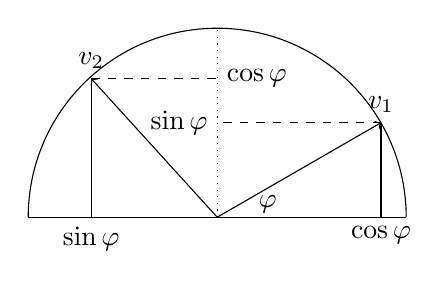
\begin{tikzpicture}[scale = 0.8]
\draw (0,0) arc (180:0:3cm);
\draw (0,0) -- (6cm,0);
\draw [->] (3cm,0) -- (1cm,2.2cm) node [above] {$v_2$};
\draw (1cm,2.2cm) -- (1cm,0) node [below] {$\sin\varphi$};
\draw [->] (3cm,0) -- (5.6cm,1.5cm) node [above] {$v_1$};
\draw (5.6cm,1.5cm) -- (5.6cm, 0) node [below] {$\cos\varphi$};
\node at (3.8cm,0.2) {$\varphi$};
\draw [dotted] (3cm,0) -- (3cm,3cm);
\draw [dashed] (5.6cm,1.5cm) -- (3cm,1.5cm) node [above,left] {$\sin\varphi$};
\draw [dashed] (1cm,2.2cm) -- (3cm,2.2cm) node [above,right] {$\cos\varphi$};
\end{tikzpicture}
\end{center}


Choose $v_2 = \begin{pmatrix}
  - \sin\varphi \\ \cos\varphi	
 \end{pmatrix}$. Then 
 \[
  \begin{pmatrix}
  | & | \\ v_1 & v_2 \\ | & | 	
  \end{pmatrix} = \begin{pmatrix}
  \cos\varphi & -\sin\varphi \\ \sin\varphi & \cos\varphi 	
 \end{pmatrix} = R_\varphi \qedhere
\]
\end{proof}


Observe that $R_\varphi^t = R_\varphi^{-1}$ (any rotation matrix is an orthogonal matrix). From the diagonalisation theory we know that $PAP^{-1} = \mathrm{diag}(\lambda_1,\lambda_2)$ where 
\[
P = \begin{pmatrix}
  | & | \\ v_1 & v_2 \\ | & | 	
  \end{pmatrix}
\]
Now $P = R_\varphi$, so we have 
\[
  \equalto{R_\varphi^{-1}AR_\varphi = \mathrm{diag}(\lambda_1,\lambda_2)}{\large R_\varphi^tAR_\varphi}
\]
So if $x = R_\varphi y$, then 
\begin{align*}
  x^tAx &= y^tR_\varphi^tAR_\varphi y\\
  &= y^tR_\varphi^{-1}AR_\varphi y
 \end{align*}
 
\[\implies x^tAx = y^t\mathrm{diag}(\lambda_1,\lambda_2)y = \lambda_1y_1^2 + \lambda_2y_2^2\]

\[(y_1,y_2)\begin{pmatrix}
 \lambda_1 & 0 \\ 0 & \lambda_2	
\end{pmatrix}\begin{pmatrix}
y_1 \\ y_2	
\end{pmatrix} = \lambda_1y_1^2 + \lambda_2y_2^2
\]


\begin{example} Same equation as before
\[
  A = \begin{pmatrix}
 5 & 2 \\ 2 & 2	
 \end{pmatrix}
\]
\[
  t^2 - 7t + 6 = (t-1)(t-6)
\]
so $\lambda_1 = 1,\, \lambda_2 = 6$. Let's find the first eigenvector (2nd follows easily since it's perpendicular). 

\[
  I - A = \begin{pmatrix}
 -4 & -2 \\ -2 & -1 	
 \end{pmatrix}\implies 
 v_1 = \frac{1}{\sqrt{5}}\begin{pmatrix}
1 \\ -2	
\end{pmatrix}
\]
($||v_1|| = 1$). Then we don't even have to calculate $v_2$, and we can take 
\[
  v_2 = \frac{1}{\sqrt{5}}\begin{pmatrix}
 2 \\ 1	
\end{pmatrix}
\]
Check: 
\[
  \frac{1}{\sqrt{5}}\begin{pmatrix}
 1 & 2 \\ -2 & 1	
\end{pmatrix}
\]
has determinant $1$. This is $R_\varphi$ from the beginning of the lecture.
\end{example}\vsp



\begin{corollary}
Any conic can be reduced to the following form:
\[
  \lambda_1y_1^2 + \lambda_2y_2^2 + d'y_1 + e'y_2 + f' 
\]
be a rotation. Here $\lambda_1,\lambda_2$ are the eigenvalues of $A = \begin{pmatrix}
 a & \frac{1}{2}b\\ \frac{1}{2}b & c	
 \end{pmatrix}$. 
\end{corollary}\vsp


Obviously $\lambda_1\lambda_2 = \det(A)$. (since the characteristic polynomial is $t^2 - (a+c)t + \det(A) = (t-\lambda_1)(t-\lambda_2)$).

Therefore if $\det(A) > 0$, then $\lambda_1,\lambda_2$ have the same sign. We complete the squares and obtain
\[
  \lambda_1z_12 + \lambda_2z_2^2 = h,\quad \mbox{ where $h \iR$}
\]
\begin{itemize}
\item  If $h > 0$, this is an ellipse. 
\item If $h < 0$, this is an imaginary ellipse.
\item If $h = 0$, this is two complex conjugate lines meeting in one real point $(0,0)$
\end{itemize}\vsp

Next, if $\det(A) < 0$, completing the square we obtain
\[
    \lambda_1z_1^2 + \lambda_2z_2^2 = h,\quad h \iR
\]
\begin{itemize}
\item  If $h > 0$ or $h< 0$, this is a hyperbola. 
\item If $h = 0$, this a pair of real lines meeting at a point. 
\end{itemize}\vsp

Finally if $\det(A) = 0$, then $\lambda_2 = 0$, $\lambda_1 \neq 0$. Complete the square for $y_1$, so we obtain
\[
  \lambda_1z_1^2 + e'y_2 + f'
\]
\begin{itemize}
\item  If $e' \neq 0$, we reduce to $\lambda_1z_1^2 + e'z_2 = 0$, which is a parabola.
\item If $e' = 0$, then $\lambda_1z_1^2 + f' = 0$. $z_1^2 = -\frac{f'}{\lambda_1}$. If RHS is positive, these are two parallel real lines. If RHS is zero, it's a double line. If RHS is negative, there are no real solutions; this is two parallel complex conjugate lines. 
\end{itemize}\vsp

\textbf{Moral}: If we can prove that our conic is non-empty and non-degenerate, then its type is uniquely determined by $\det(A)$. 
 \begin{itemize}
\item   $\det(A) > 0 \implies$ ellipse. 
\item  $\det(A) > 0 \implies$ parabola. 
\item  $\det(A) > 0 \implies$ hyperbola.
  \end{itemize}








 



\subsektion{Quadric Surfaces}\vsp
 
\begin{definition}
A \emph{quadric surface} is \lecturemarker{19}{2/12} a surface in $\R^3$ defined by an eqn of degree $2$: 
\[
  ax_1^2 + bx_2^2 + cx_3^2 + dx_1x_2 + ex_1x_2 + fx_2x_3 + gx_1 + hx_2 + jx_3 + k = 0
\]
\end{definition}

\textbf{Task:} Use an orthogonal transformation, ideally a rotation, to reduce this equation to one of standard form.

\subsubsektion{Non-denerate forms}
Here are non-degenerate forms, with $0 \neq a,b,c\iR$:


(1) Ellipsoid:
\[\frac{x_1^2}{a^2} + \frac{x_2^2}{b^2} + \frac{x_3^2}{c^2} = 1\]

\begin{center}
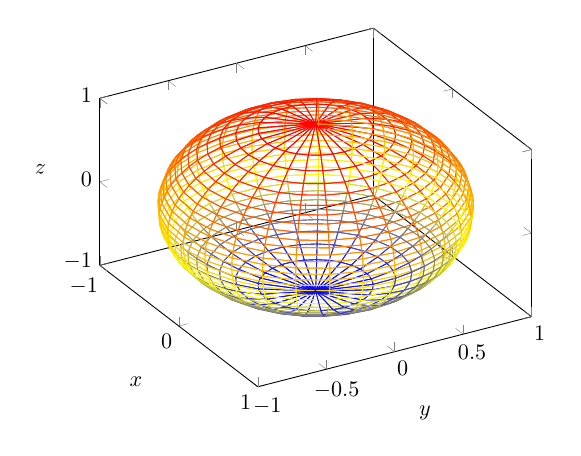
\begin{tikzpicture}[scale = .8]
    \begin{axis}[
            xmin=-1,xmax=1,
            ymin=-1,ymax=1,
            zmin=-1,zmax=1,
            xlabel={$x$},
            ylabel={$y$},
            zlabel={$z$},
            zlabel style={rotate=90},
            view={60}{40}]
  \addplot3[mesh,samples=30,domain=-1:1,y domain=0:2*pi]({sqrt(1-x^2) * cos(deg(y))},
{sqrt( 1-x^2 ) * sin(deg(y))},
x);    \end{axis}
\end{tikzpicture}
\end{center}


  
(2) Hyperboloid of one sheet: 
\[\frac{x_1^2}{a^2} + \frac{x_2^2}{b^2} - \frac{x_3^2}{c^2} = 1\]

\begin{center}
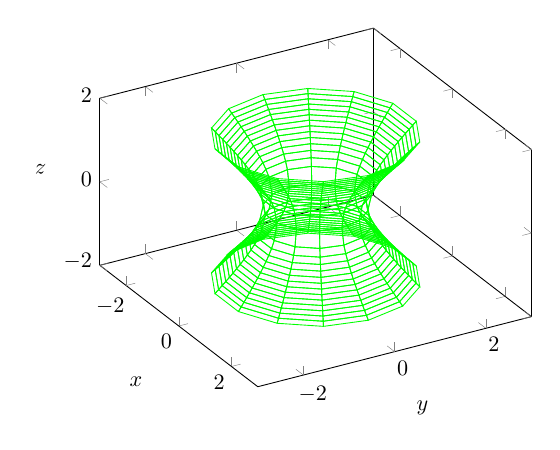
\begin{tikzpicture}[scale = .8]
    \begin{axis}[
            xmin=-3,xmax=3,
            ymin=-3,ymax=3,
            zmin=-2,zmax=2,
            xlabel={$x$},
            ylabel={$y$},
            zlabel={$z$},
            zlabel style={rotate=90},
            view={60}{40}]
  
        % x^2+y^2-z^2=1
        \addplot3[mesh,green,domain=1:2,y domain=0:2*pi,samples=15]({x*cos(deg(y))},{x*sin(deg(y))},{sqrt(x^2-1)});    
        \addplot3[mesh,green,domain=1:2,y domain=0:2*pi,samples=15]({x*cos(deg(y))},{x*sin(deg(y))},{-sqrt(x^2-1)});    

    \end{axis}
\end{tikzpicture}
\end{center}


(3) Hyperboloid of two sheets: 
\[-\frac{x_1^2}{a^2} - \frac{x_2^2}{b^2} + \frac{x_3^2}{c^2} = 1\]

\begin{center}
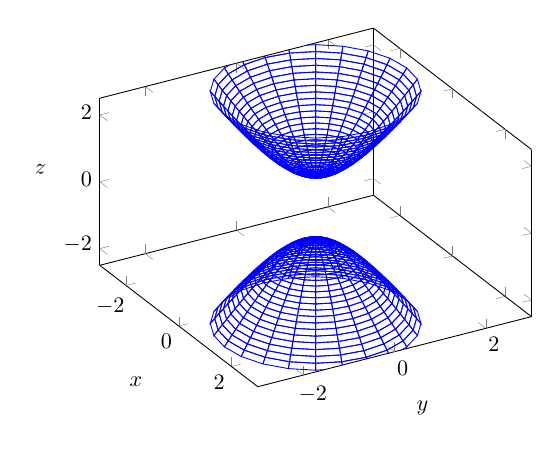
\begin{tikzpicture}[scale = .8]
    \begin{axis}[
            xmin=-3,xmax=3,
            ymin=-3,ymax=3,
            zmin=-2.5,zmax=2.5,
            xlabel={$x$},
            ylabel={$y$},
            zlabel={$z$},
            zlabel style={rotate=90},
            view={60}{40}]
  
         % x^2+y^2-z^2=-1
        \addplot3[mesh,blue,domain=0:2,y domain=0:2*pi]({x*cos(deg(y))},{x*sin(deg(y))},{2*sqrt(x^2+1)-1});    
        \addplot3[mesh,blue,domain=0:2,y domain=0:2*pi]({x*cos(deg(y))},{x*sin(deg(y))},{-2*sqrt(x^2+1)+1});    

    \end{axis}
\end{tikzpicture}
\end{center}


(4) Elliptic Paraboloid: 
\[x_3 = \frac{x_1^2}{a^2} + \frac{x_2^2}{b^2}\]

\begin{center}
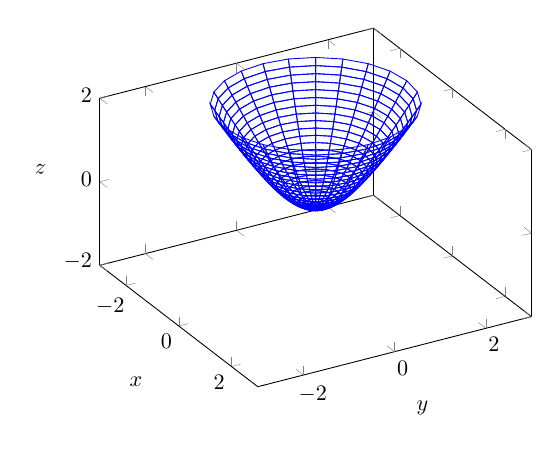
\begin{tikzpicture}[scale = .8]
    \begin{axis}[
            xmin=-3,xmax=3,
            ymin=-3,ymax=3,
            zmin=-2,zmax=2,
            xlabel={$x$},
            ylabel={$y$},
            zlabel={$z$},
            zlabel style={rotate=90},
            view={60}{40}]
  
         % x^2+y^2-z^2=-1
        \addplot3[mesh,blue,domain=0:2,y domain=0:2*pi]({x*cos(deg(y))},{x*sin(deg(y))},{2*sqrt(x^2+1)-2});    
    \end{axis}
\end{tikzpicture}
\end{center}



(4) Hyperbolic Paraboloid: 
\[x_3 = \frac{x_1^2}{a^2} - \frac{x_2^2}{b^2}\]

\begin{center}
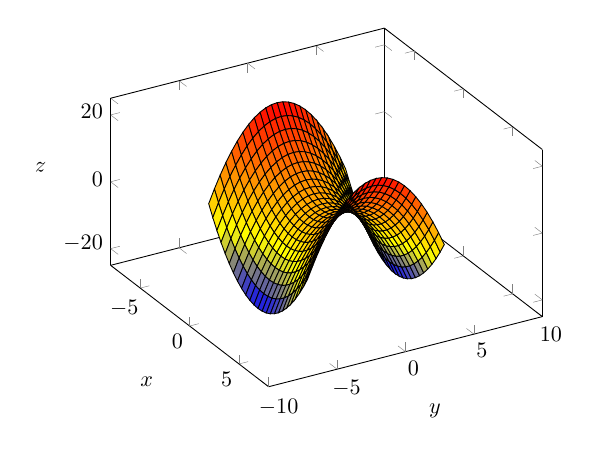
\begin{tikzpicture}[scale = .8]
    \begin{axis}[
            xmin=-8,xmax=8,
            ymin=-10,ymax=10,
            zmin=-25,zmax=25,
            xlabel={$x$},
            ylabel={$y$},
            zlabel={$z$},
            zlabel style={rotate=90},
            view={60}{40}]
\addplot3 [surf,shader=flat,draw=black] {.8*x^2-y^2};
    \end{axis}
\end{tikzpicture}
\end{center}


\textbf{Some examples of degenerate quadrics}

(5) Cone: 
\[\frac{x_1^2}{a^2} + \frac{x_2^2}{b^2} - \frac{x_3^2}{c^2} = 0\]

\begin{center}
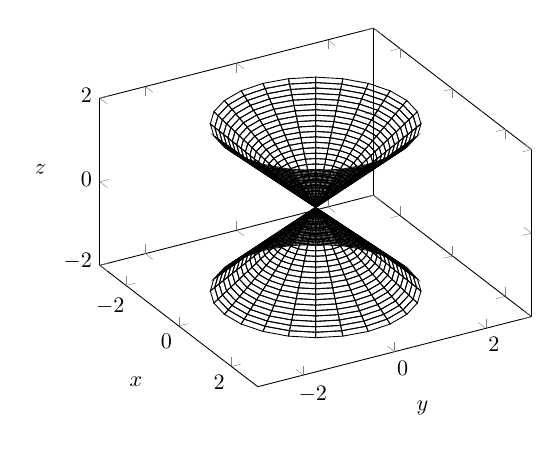
\begin{tikzpicture}[scale = .8]
    \begin{axis}[
            xmin=-3,xmax=3,
            ymin=-3,ymax=3,
            zmin=-2,zmax=2,
            xlabel={$x$},
            ylabel={$y$},
            zlabel={$z$},
            zlabel style={rotate=90},
            view={60}{40}]
        \addplot3[mesh,black,domain=0:2,y domain=0:2*pi]({x*cos(deg(y))},{x*sin(deg(y))},{x});    
        \addplot3[mesh,black,domain=0:2,y domain=0:2*pi]({x*cos(deg(y))},{x*sin(deg(y))},{-x});    
    \end{axis}
\end{tikzpicture}
\end{center}

(6) Elliptic cylinder 
\[\frac{x_1^2}{a^2} + \frac{x_2^2}{b^2} = 1\]

Similarly there are hyperbolic and parabolic cylinders, etc. \emph{You will not be expected to know all the quadrics for the exam.} 


\subsektion{Reducing Quadrics}

\textsc{Step 1.} Write the equation in matrix form. 
\[
  x = \begin{pmatrix}
 x_1 \\ x_2 \\ x_3	
 \end{pmatrix}\implies x^tAx + (ghj)x + k = 0
\]
where 
\[
  A = \begin{pmatrix}
 a & \frac{d}{2} & \frac{e}{2} \\ \frac{d}{2} & b & \frac{f}{2} \\ \frac{e}{2} & \frac{f}{2} & c 	
 \end{pmatrix}
\]\vsp

\textsc{Step 2.} Find the eigenvalues of $A$. In fact any symmetric $3 \times 3$ matrix has three real eigenvalues: $\det(tI-A) = (t-\lambda_1)(t-\lambda_2)(t-\lambda_3)$ where $\lambda_i\iR$. (See sheet 8 for proof). 

We've seen before that $\lambda_i \neq \lambda_j$ and $v_i$ is an eigenvector of $\lambda_i$, $v_j$ is an eigenvector for $\lambda_j$, then $v_i$ is perpendicular to $v_j$, i.e. $v_i \cdot v_j = 0$. So if $\lambda_1 \neq \lambda_2 \neq \lambda_3$, then we can find $v_1,v_2,v_3$ of length $1$: $||v_1|| = ||v_2|| = ||v_3|| = 1$. These vectors will be perpendicular automatically to each other. The same also works in the general case.\\ 

\textsc{Step 3.} 
\[
  P = \begin{pmatrix}
  | & | & | \\ v_1 & v_2 & v_3 \\ | & | &| 	
 \end{pmatrix}
\]
Then $P$ is an orthogonal matrix, i.e. $P^tP =I \implies P^t = P^{-1}$, since $||v_i|| = 1, i = 1,2,3$ and $v_i \cdot v_j = 0$ when $i \neq j$.\\


\textsc{Step 4.} Since $P^{-1} = P^t$, $x = Py$ where $y=(y_1,y_2,y_3)^t$. So the equation now looks as follows:
\[
  x^tAx = y^tP^{-1}APy
\]
But $P^{-1}AP$ is the diagonal matrix \[
  D = \begin{pmatrix}
 \lambda_1 & 0 & 0\\ 0 & \lambda_2 & 0 \\ 0 & 0 & \lambda_3	
 \end{pmatrix}
\]
Therefore 

\begin{align*}
  x^tAx &= y^tP^{-1}APy \\
  &= y^t\mathrm{diag}(\lambda_1,\lambda_2,\lambda_3)y\\
  &= \lambda_1y_1^2 + \lambda_2y_2^2 + \lambda_3y_3^2
\end{align*}
The whole equation now is 
\[
  \lambda_1y_1^2 + \lambda_2y_2^2 + \lambda_3y_3^2
+ g'y_1 + h'y_2 + j'y_3 + k = 0
\]
If $\lambda_1\lambda_2\lambda_3 \neq 0$, complete the squares and get one of two hyperboloids, an ellipsoid, or a degenerate quadric. If $\lambda_1\lambda_2 \neq 0, \lambda_3 = 0$ we get a paraboloid (one of two types) or a degenerate.\\

\begin{example} Reduce to standard form
\[
  2x_1x_2 + 2x_1x_3 - x_2 - 1 = 0
\]
Using an orthogonal transformation and a translation.	

1. $x^tAx - x_2 - 1= 0$, where
\[
  A = \begin{pmatrix}
 0 & 1 & 1 \\ 1 & 0 & 0 \\ 1 & 0 & 0 	
 \end{pmatrix}
\]

2. 
\begin{align*}
  \det\begin{pmatrix}
t & -1 & - 1\\ -1 & t & 0 \\ -1 & 0 & t	
\end{pmatrix} &= t^3  -2t\\
&= t(t-\sqrt{2})(t+\sqrt{2})
\end{align*}

If this quadric is non-degenerate, it myst be a hyperbolic paraboloid (since $\lambda_1 = 0, \lambda_2 = \sqrt{2}$ and $\lambda_3 = -\sqrt{3} < 0$)\\

3. Find the eigenvectors $\lambda_1 = 0$, solving $Ax = 0$: 
\[
  \begin{amatrix}{3}
  	0 & 1 & 1 & 0 \\ 
  	1 & 0 & 0 & 0\\
  	1 & 0 & 0 & 0 
  \end{amatrix}
\]
Solving we find $v_1 = \frac{1}{\sqrt{2}}\begin{pmatrix}
0 \\ 1 \\-1	
\end{pmatrix}$. 

For $\lambda_2 = \sqrt{2}$, solving $Ax = 0$: 
\[
  \begin{amatrix}{3}
  	\sqrt{2} & -1 & -1 & 0 \\ 
  	-1 & \sqrt{2} & 0 & 0\\
  	-1 & 0 & \sqrt{2} & 0 
  \end{amatrix}
\]
Solving we find $v_2 = \frac{1}{2}\begin{pmatrix}
\sqrt{2} \\ 1 \\ 1	
\end{pmatrix}$.

$\lambda_3 = -\sqrt{3} \implies v_3 = \frac{1}{2}\begin{pmatrix}
-\sqrt{2} \\ 1 \\ 1	
\end{pmatrix}$.\\


4. Hence 
\[
  P = \begin{pmatrix}
 0 & \frac{\sqrt{2}}{2} & - \frac{\sqrt{2}}{2}\\[.1cm]
 +\frac{1}{\sqrt{2}} & \frac{1}{2} & \frac{1}{2}\\[.1cm]
 -\frac{1}{\sqrt{2}} & \frac{1}{2} & \frac{1}{2}	
 \end{pmatrix}
\]
\begin{align*}
  &\implies y^tAy + (0,-1,0)Py -1\\
  &= \sqrt{2}(y_2-\alpha)^2 - \sqrt{2}(y_3 - \beta)^2+ \frac{1}{\sqrt{2}}(y_1 - \delta)
\end{align*}
where $\alpha,\beta,\delta \iR$. So this is a non-degenerate quadric, hence a hyperbolic paraboloid. 
\end{example}




\begin{center}

\includegraphics[width=6.5cm]{cartoon5.jpg}	
\end{center}






\sektion{Geometry in $\R^3$}

A vector \lecturemarker{20}{25/11} $x = (x_1,x_2,x_3) \iR^3$ is such that 
\begin{itemize}
\item a point $P$
\item a vector $\vec{OP}$
\item any vector $\vec{AB}$ of same length and direction as $\vec{OP}$.	
\end{itemize}\vspace*{5pt}

\begin{definition}
The \emph{length} of $x = (x_1,x_2,x_3)$ is
\begin{align*}
  ||x|| &= \sqrt{x_1^2 + x_2^2 + x_3^2}\\
  &= |OP|
\end{align*}
\end{definition}
%\begin{center}
%\begin{tikzpicture}
%\draw[->] (0,0) -- (4,0);
%\draw[->] (0,0) -- (0,3);
%\draw [->] (0,0) -- (2,2);	
%\end{tikzpicture}
%\end{center}

\[
  (x_1,x_2,x_3) + (y_1,y_2,y_3)
  = (x_1+y+1,x_2+y_2,x_3+y_3)
\]
\[
  \lambda(x_1,x_2,x_3) = (\lambda x_1,\lambda x_2, \lambda x_3)
\]

%\begin{center}
%\begin{tikzpicture}
%	\draw[<->] (0,0) -- (3,0) node at (1.5,-0.3) {$x$};
%\draw[<->] (3,0) -- (4.5,2.5) node at (4,1) {$y$};
%\draw[<->] (0,0) -- (4.5,2.5) node at (2,1.5) {$x + y$};	
%\end{tikzpicture}
%\end{center}


\begin{definition}[Lines of $\R^3$]
$L = \{ a +\lambda u: \lambda \iR\}$ is a line in $\R^3$.	
\end{definition}

%DIAGRAM OF LINE 

\begin{definition}[Dot product]
For $x,y \iR^3$\[
  x\cdot y = x_1y_1 + x_2y_2 + x_3y_3\]
\end{definition}

\begin{proposition}
For $x,y\iR^3$ we have $x \cdot y = ||x|| \cdot||y|| \cdot \cos\theta$ 
%picture of prop 9.1
\end{proposition}\vspace*{5pt}

\subsektion{Planes}
$n = a$ is a normal vector for the plane. 

$x\cdot y = 0 \iff x$ and $y$ are perpendicular. So $x-a$ is perpendicular to $n \iff (x-a)\cdot n = 0$. This is the equation of a plane. 

Now $u \cdot (v+w) = u\cdot v + u\cdot w$ so $(x-a) \cdot n = x\cdot n - a\cdot n$. So the equation of the plane is 
\[x\cdot n = a\cdot n\]
Write $a\cdot n = c$, a scalar, so you get
\[x\cdot n = c\]
Write $n = (n_1,n_2,n_3)$ then 
\[
  n_1x_1 + n_2x_2 + n_3x_3 = c
\]

\begin{example}
	We need $a,n$. $a = (e,e,0)$ and $n = (0,0,\pi)$. Then $(x-a) \cdot n = 0$, so $x\cdot n = a\cdot n$. Then 
	\begin{align*}
  a\cdot n &= (e,e,0) \cdot (0,0,n)\\
  &= 0
\end{align*}
So the equation is 
\begin{align*}
  (x_1,x_2,x_3)\cdot(0,0,n) &= 0\\
  \pi x_3 &= 0\\
  \implies x_3 &= 0
\end{align*}
\end{example}\vsp

\begin{proposition}~\\[0.1cm]
(i) The intersection of two planes is 
\begin{itemize}
\item Nothing
\item A line 
\item A plane (if the two planes are the same)
\end{itemize}
(ii) If $A,B,C$ are $3$ points which don't lie on a common line, then there is a unique plane through $A,B,C$.
\end{proposition}
\emph{Proof.} Problem sheet 7.

Let $e_1 = (1,0,0)$, $e_2 = (0,1,0)$ and $e_3 = (0,0,01)$, so $(x_1,x_2,x_3) = x_1e_1 + x_2e_2 + x_3e_3$.\\

\begin{definition}[Vector product]
	The vector product = cross product of $a,b$ is 
\begin{align*}
  a \times b &= \begin{vmatrix}
 e_1 & e_2 & e_3\\
 a_1 & a_2 & a_3\\
 b_1 & b_2 & b_3	
 \end{vmatrix}\\
 &= e_1(a_2b_3 - a_3b_2) - e_2(a_1b_3 - a_3b_1) + e_3(a_1b_2 - a_2b_1)\\
 &= (a_2b_3 - a_3b_2, a_3b_1 - a_1b_3, a_1b_2 - a_2b_1)
\end{align*}

\end{definition}\vspace*{5pt}

\begin{example}
\begin{align*}
  (1,-1,0) \times (3,0,1)
  &= \begin{vmatrix}
 e_1 & e_2 & e_3\\
 1 & -1 & 0\\
 3 & 0 & 1	
 \end{vmatrix}\\
 &= (-1,1,3)
\end{align*}
\end{example}\vsp

\begin{proposition}
$a\times b$ is perpendicular to both $a,b$. 	
\end{proposition}
\begin{proof}
	\begin{align*}
  a \cdot (a \times b) &= \begin{vmatrix}
 a_1& a_2 & a_3\\
 a_1 & a_2 & a_3\\
 b_1 & b_2 & b_3	
 \end{vmatrix}\\
 &= 0
\end{align*}
Similarly $b \cdot (a \times b) = 0$.
\end{proof}


\begin{proposition}
\begin{enumerate}
\item $e_1 \times e_2 = e_3$, $e_2 \times e_3 = e_1$, $e_3 \times e_1 = e_2$
\item $a \times a = 0$
\item $b \times a = -a \times b$
\item $(\lambda a) \times b= \lambda(a \times b) = a \times (\lambda b)$ for any scalar $\lambda \iR$
\item $a \times (b + c) = a \times b + a \times c$	
\end{enumerate}
\end{proposition}
\begin{proof} Use properties of determinants:\\
(i) \begin{align*}
  e_1 \times e_2 &= \begin{vmatrix}
 e_1 & e_2 & e_3\\
 1 & 0 & 0\\
 0 & 1 & 0	
 \end{vmatrix}\\
 &= e_3 = (0,0,1)
\end{align*}

(ii) $a = (a_1,a_2,a_3)$, then 
\begin{align*}
  a \times a &= \begin{vmatrix}
 e_1 & e_2 & e_3\\
 a_1 & a_2 & a_3\\
 a_1 & a_2 & a_3	
 \end{vmatrix}\\
 &= 0 = (0,0,0)
\end{align*}

(iii) 

	
\end{proof}



%\subsektion{Cross product} 


\begin{proposition}
For any {\normalfont \lecturemarker{21}{27/11}}vectors $a,b \iR^3$ we have 
\begin{align*}
  ||a\times b|| &= ||a|| \cdot ||b|| \cdot |\sin\theta|\\
 &= \text{ the area of a parallelogram } OABC
\end{align*}
\end{proposition}

%\begin{center}
%\begin{tikzpicture}
%\draw[<->] (0,0) -- (3,0) node at (1.5,-0.3) {$x$};
%\draw[<->] (3,0) -- (4.5,2.5) node at (4,1) {$y$};
%\draw[<->] (0,0) -- (4.5,2.5) node at (2,1.5) {$x + y$};	
%\end{tikzpicture}
%\end{center}
%

\begin{proof}
Squaring both sides: 
\[
  \implies ||a\times b||^2 = (a_2b_3 - a_3b_2)^2 + (a_3b_1 - b_1a_3)^2 + (a_1b_2 - a_2b_1)^2
\]
\[
  \text{Area} = ||a|| \cdot ||h|| = ||a|| \cdot ||b|| \cdot |\sin\theta|
\]
\begin{align*}
  ||a||^2 \cdot ||b||^2 \cdot(1-\cos^2\theta) &= ||a||^2||b||^2 - (||a||||b||\cos\theta)^2\\
  &= (a_1^2 + a_2^2 + a_3^2) \cdot(b_1^2 + b_2^2 + b_3^2) - (a\cdot b)^2\\
  &= (a_1^2 + a_2^2 + a_3^2) \cdot(b_1^2 + b_2^2 + b_3^2) - (a_1b_1 + a_2b_2 + a_3b_3)^2\\
  &= a_1^2b_2^2 + a_2^2 + b_1^2 - 2a_1a_2b_1b_2 + \dots + \text{(similar terms)}
\end{align*}
Check that the two expressions are identitical. 
\end{proof}

\emph{Remark.} $a \times b$ is a vector perpendicular to the plane through $O,\, a$ and $b$ of length that's equal to the area of the parallelogram build on $O,a,b$.\\

\begin{example}
Find the area of a triangle in $\R^3$ with corners $(1,0,0),\,(1,1,0),\,(0,1,1)$.\\

Answer: Area $= \frac{1}{2}$(length of $a \times b$) where $a = (0,1,0),\, b = (-1,1,1)$

\begin{center}
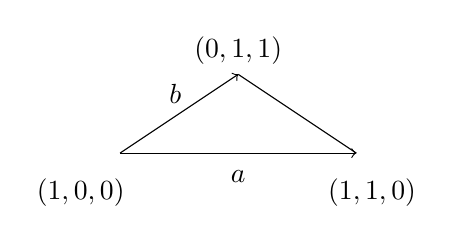
\begin{tikzpicture}
\draw[->] (0,0) -- (3,0) node at (3.2,-0.5) {$(1,1,0)$};	
\draw[->] (0,0) -- (1.5,1) node [above] {$(0,1,1)$};
\draw (1.5,1) -- (3,0); 
\node at (-0.5,-0.5) {$(1,0,0)$};
\node at (1.5,-0.3) {$a$};
\node at (0.7,.75) {$b$};
\end{tikzpicture}
\end{center}
	
\begin{align*}
  \det\begin{pmatrix}
e_1 & e_2 & e_3 \\ 0 & 1 & 0 \\ -1 & 1 & 1	
\end{pmatrix}
&= e_1 -e_2 \cdot 0 + e_3\\
&= e_1 + e_3\\
&= (1,0,1) = a \times b
\end{align*}

Hence $||a\times b|| = \sqrt{2} \implies$ area of triangle is $\frac{\sqrt{2}}{2}$.
\end{example}\vsp 


\subsubsektion{Volume}
\begin{proposition}
The volume of the parallelepiped built on $a,b,c$ equals $|a\cdot (b\times c)|$
\[
  = \left|det\begin{pmatrix}
 	a_1& a_2 & a_3\\ b_1 & b_2 & b_3\\ c_1 & c_2 & c_3
 \end{pmatrix}\right|
\]

\end{proposition}
\begin{proof}
Let's show that vol$ = |a\cdot (b \times c)|$. By previous proposition the area of the base is $(b\times c) = ||b \times c||\cdot n$ where $n$ is a unit normal to the plane through $0, b$ and $c$. Therefore
\[
  |a\cdot (b \times c)| = ||a|| \cdot || b\times c|| \cdot |\cos\theta|
\]
where $\theta$ is the angle between $a$ and $n$. But $||a||\cdot|\cos\theta|$ is the height of the parallelepiped. So we proved that vol$ = |a\cdot (b \times c)|$. 

Finally 
\[
  \det\begin{pmatrix}
	a_1&a_2 & a_3 \\ b_1 & b_2 & b_3\\ c_1 & c_2 & c_3
\end{pmatrix}
\]


	
\end{proof}

\subsubsektion{Properties of scalar triple product}

\begin{proposition}
For any $a,b,c \iR^3$ we have 

(i) $a \cdot (b \times c) = c\cdot (a \times b) = b\cdot (c \times a)$

(ii) $a,b,c$ are coplanar ($= 0,a,b,c$ belong to a plane) if and only if 
\[
  \det\begin{pmatrix}
a_1 & a_2 & a_3 \\ b_1 & b_2 & b_3 \\ c_1 & c_2 & c_3 	
\end{pmatrix} = 0
\]
\end{proposition}

\begin{proof}
(i) 
\begin{align*}
  \det\begin{pmatrix}
a_1 & a_2 & a_3 \\ b_1 & b_2 & b_3 \\ c_1 & c_2 & c_3 	
\end{pmatrix} &=   -\det\begin{pmatrix}
a_1 & a_2 & a_3\\ c_1 & c_2 & c_3 	 \\ b_1 & b_2 & b_3 
\end{pmatrix} = \det\begin{pmatrix}
 c_1 & c_2 & c_3\\ a_1 & a_2 & a_3	 \\ b_1 & b_2 & b_3 
\end{pmatrix}
\end{align*}
Hence $a \cdot (b \times c) = c\cdot (a \times b)$. Similarly we can probe that $c \cdot(a \times b) = b\cdot (c \times a)$.\\

(ii) $a,b,c$ are coplanar $iff$ volume of parallelepiped built on $a,b,c$ is $0 \iff \det = 0$.
\end{proof}\vsp

\begin{proof}[Alternative Proof of (ii).]
	Any plane through $0$ can be given by 
	\[
  m_1x_1 + m_2x_2 + m_3x_3 = 0
\]
(at least one co-efficient $m_i \neq 0$). Then 
\[
  \begin{pmatrix}
  	a_1 & a_2 & a_3 \\ b_1 & b_2 & b_3 \\ c_1 & c_2 & c_3 	
  \end{pmatrix}\begin{pmatrix}
	m_1 \\ m_2 \\ m_3
\end{pmatrix} = 0
\]
Since $a,b,c$ are contained in this plane. This system of linear equations has a non-zero solution. Therefore $\det = 0$. 

This argument can be reversed; conversely if $\det = 0$, then there is a non-zero solution which gives a plane though $0,a,b,c$. 
\end{proof}\vsp


\begin{example}
\emph{Are the points $(1,0,0),(1,1,1),(1,2,3),(2,3,4)$ in the same plane? }

Let $a = (0,1,1), b = (0,2,3) , c = (1,3,4)$. 
\[
  \det\begin{pmatrix}
0 & 1 & 1 \\ 0 & 2 & 3 \\ 1 & 3 & 4	
\end{pmatrix} = \det\begin{pmatrix}
1 & 1 \\ 2 & 3 	
\end{pmatrix} = 1
\]
This is not $0$, hence the four points do not belong to a common point. 
\end{example}\vsp


\emph{What is $(a \times b) \times c$?}

We know that this is perpendicular to the plane through $a \times b$ and $c$. Hence $(a \times b) \times c$ is in the plane through $0,a,b$, so the triple vector product $(a \times b) \times c) = (k_1)a + (k_2)b$.\\


\begin{proposition}{\normalfont \lecturemarker{22}{28/11} }
For $a,b, c\iR^3$:

(i) $(a \times b) \times c) = (a \cdot c) b - (b\cdot c)a$

(ii) $a \times (b \times c) = (a\cdot c)b - (a\cdot b)c$
\end{proposition}

\emph{Remark.} Vector product is not associative! 

\begin{proof}
(i) $a \times b= (a_2b_3 - a_3b_2, a_3b_1 - a_1b_3, a_1b_2 - a_2b_1)$. $(a\times b) \times c = $ the $x_1$ coordinate of $(a \times b) \times c$ which is $(a_3b_1 - a_1b_3)c_3 - (a_1b_2 - a_2b_1)c_2$. The $x_1$ coordinate of RHS is $(a_1c_1 + a_2c_2 + a_3c_3)b_1 - (b_1)1 + b_2c_3 + b_3c_3)a_1$. Hence LHS = RHS. Similarly, check that $x_2$ and $x_3$ coordinate of LHS and RHS are equivalent. \\

(ii) 
\begin{align*}
  a \times (b \times c) &= -(b \times c) \times a)\\
  \implies &= (c \times b) \times a)\\
  \implies &= (c \cdot a)b - (b\cdot a)c\\
  &= (a\cdot b)b - (a\cdot b)c\qedhere 
\end{align*}
\end{proof}\vsp

\emph{Remark.} Use this proposition to establish the Jacobi identity:
\[
  (a \times b) \times c + (c \times a)\times b + (b \times c) \times a = 0
\]
This, with the property that $a \times b = - b \times a$ turn $\R^3$ into a \emph{Lie Algebra}.\\

\begin{example}
$a,b,c,d \iR^3$. What is $(a \times b)\cdot(c \times d)$?\\

Answer: Call $u = a \times b$. We proved that
 \begin{align*}
   u \cdot(c \times d) &= d\cdot(u \times c)\quad \text{(prop 9.7)}\\
   &= d\cdot((a \times b) \times c) \\
   &= d\cdot((a\cdot c)b - (b\cdot c)a)\quad \text{(prop 9.8)} \\
   &= (a\cdot c) \cdot(b\cdot d) - (b\cdot c)(a\cdot d)
\end{align*}
\end{example}\vsp


\begin{proposition}
Let $a \iR^3$, $a \neq 0$. Then $b \times a= 0$ if and only if $b = \lambda a$ for some $\lambda \iR$. 	
\end{proposition}

\begin{proof}
If $b = \lambda a$ then $b \times a = \lambda a \times a =0$. Conversely assume that $b \times a= 0$. Then certainly $(a \times (b \times a) = a \times 0 = 0$. Then $a \times(b \times a) = (a\cdot a)b - (a\cdot b)a$. We know that this is zero, but $(a\cdot a) = ||a||^2 \neq 0$, since $a \neq 0$, so $b = \frac{(a\cdot b)}{||a||^2}a$.	
\end{proof}\vsp


\begin{proposition}
Let $a,b\iR^3$. Assume $a \neq 0$. Then the set of $x \iR^3$ such that $(x-b) \times a = 0$ is the line $\{b + \lambda a ~|~ \lambda \iR\}$.	
\end{proposition}


\begin{proof}
$(x-b) \times a = 0 \iff x -b = \lambda a$ for some $\lambda \iR$ by the previous proposition.	
\end{proof}


\subsektion{Rotations in $\R^3$}

The axis of rotation is the line in $\R^3$ such that every point of this line is fixed by the rotation. We write a rotation by a $3 \times 3$ matrix $P$ such that a vector $(x_1,x_2,x_3)^t$ goes to $P(x_1,x_2,x_3)^t$. 

\textbf{Claim:}

(i) $P$ is an orthogonal matrix, i.e. $P^t = P^{-1}$

(ii) Any orthogonal matrix has determinant $1$ or $-1$. If $\det P = 1$, then this is a rotation matrix. 

(iii) The axis is $\{\lambda v ~|~ \lambda \iR\}$, where $v$ is an eigenvector of $P$ with eigenvalue $1$, i.e. $Pv = v$

(iv) To find the angle, we take any unit vector $w$ perpendicular to the axis, i.e. $w \cdot v = 0$. Then calculate $w \cdot Pw = ||w||\cdot||Pw||\cos\theta = \cos\theta$. 



\vspace*{2cm}

\begin{center}

\includegraphics[width=10cm]{cartoon4.png}
\end{center}









	


\sektion{Vector spaces}

We've \lecturemarker{23}{4/12} seen $\R^2$ and $\R^3$. Similarly, we can work with $\R^n = \{(x_1,\dots,x_n)~|~ x_i\iR\}$. In the same way we can do linear algebra in $\C^n = \{x_1,\dots,x_n ~|~ x_i \iC\}$. In this case ``scalars" mean ``complex numbers". The same methods work equally well for binary vectors. 

\textbf{Notation.} $\mathbb{F}_2 = \{0,1\}$ is the binary field such that:
\begin{align*}
  0 + 0 &= 1 + 1 = 0\\
  1 + 0 &= 0 + 1 = 1\\
  0 \times 0 &= 1 \times 0 = 0 \times 1 = 0\\
  1 \times 1 &= 1
\end{align*}

So we have three notions of scalars: $\R,\,\C,\,\mathbb{F}_2$. 


\emph{What is $(\mathbb{F}_2)^n$?}


$(\mathbb{F}_2)^n = \{(x_1,\dots,x_n) ~|~ x_i \in \mathbb{F}_2\}$

\[
  (x_1,\dots,x_n) + (y_1,\dots,y_n) = (x_1 + y_1,x_2+y_2,\dots,x_n+y_n)
\]
Here $+$ standard for binary addition, e.g. $(1,0) + (1,1) = (0,1)$. 

If $\lambda \in \mathbb{F}_2$, then $\lambda(x_1,\dots,x_n) = (\lambda x_1,\dots,\lambda x_n)$. 

Now let $F$ be one of $\R, \C$ or $\mathbb{F}_2$. I will refer to $F$ as a \emph{field}. 


\subsubsektion{Rules satisfied by addition of vectors}
For any $u,v,w \in V$ [$V$ is in $\R, \C$ or $\mathbb{F}_2$], we have 
\begin{enumerate}
\item[\underline{A1}] $u + (v+w) = (u+v) + w$ 
\item[\underline{A2}] $u + 0 = 0 + u = u$, $0 = (0,0,\dots,0)$
\item[\underline{A3}] $u+(-u) = 0$, $u = (u_1,\dots,u_n)\, -u = (-u_1,\dots,-u_n)$
\item[\underline{A4}] $u + v = v+u$
\end{enumerate}\vspace*{10pt}

\subsubsektion{Rules satisfied by scalar multiplication}
For any $\lambda, \mu \in F$ and any $u,v \in V$ we have:
\begin{enumerate}
\item[\underline{S1}] $\lambda(u+v) = \lambda u + \lambda v$ 
\item[\underline{S2}] $(\lambda + \mu)u = \lambda u + \mu u$
\item[\underline{S3}] $\lambda(\mu u) = (\lambda \mu) u$
\item[\underline{S4}] $1u = u$
\end{enumerate}\vspace*{10pt}

%A general definition of a vector space $V$ over $F$: \\

\begin{definition}[Vector space $V$ over $F$]
Let $F$ be a field (i.e. $\R, \C$ or $\F_2$) and let $V$ be a set, the elements of which are called \emph{vectors}. Suppose we have addition in $V$ i.e. a function $V \times V \to V$ and multiplication by a scalar, i.e. a function $F \times V \to V$ and an elenet of $V$ called \emph{zero} such that the properties A1-A4 and S1-S4 all hold. 	
\end{definition}

\begin{examples}~\\[-.3cm]

(1) $\R^n, \C^n, (\F_2)^n$\\

(2) Let $S$ be any set. Consider all functions $S \to |R$. Let's define the structure of a vector space on Functions$(S,\R)$.

If $f_1: S \to \R$ and $f_2: S \to \R$ are functions, then $f_1 + f_2$ is a function such that for any element $s \in S$, we have $(f_1 + f_2)(s) = f_1(s) + f_2(s)$. The zero element of Functions$(S,\R)$ is the zero function, i.e. the function that is equal to zero $\, \forall s \in S$. If $f \in \mathrm{Functions}(S,\R)$ then $-f$ is the function such that $(-f)(s) = -f(s)$,$\,\forall s \in S$.

It's clear that A1-4 hold. Now lets define scalar multiplication: $\lambda\iR$, $f \in \mathrm{Functions}(s,\R)$ then $\lambda f$ is the function such that $(\lambda f)(s)= \lambda \cdot f(s),\,\forall s$. 

Check that S1-4 hold, e.g. let's check S4. $\lambda(\mu f)$ is the function such that $\forall s \in S$ we have $(\lambda(\mu f))(s) = \lambda \mu f(s)$, which is the same as the value of the function $(\lambda \mu)\cdot f$.\\ 

(3) Similarly the set of functions from $S$ to $F$ is a vector space over $F$.\\

(4) Let's be more specific. Let $S = \R$. Consider Functions$(\R,\R)$, e.g. 

%picture of random function <= vector space is huge

So consider just polynomial functions. This is a subset of the set of all functions $\R \to \R$. Addition of polynomials is again a polynomial, and a scalar of a polynomial is also a polynomial. The set of polynomials is a \emph{subspace} of the vector space of all functions $\R \to \R$. 

Polynomials \emph{inherit} addition and scalar multiplication from Functions$(\R, \R)$, they are closed under these operations. Hence \[\R[x] = \{\text{the set of all polynomials with real coeficients}\}\] is a vector space over $\R$. We can also check A1-4 and S1-4 for polynomials directly. \\[-.2cm]

(5) Now consider polynomials of degree up to $d$, where $d$ is a fixed positive integer. This set is closed under addition and scalar multiplication so it's also a vector space over $\R$. 

e.g. $d=0$ is the space of polynomials of degree $0 = \R$. $d=1$ is $ax + b$. So addition is $(ax + b) + (a'x+b) = (a+a')x  + (b + b')$ and multiplication is $\lambda(ax +b) = \lambda a x + \lambda b$. So the space of linear polynomials can be identified with $\R^2$. Similarly, the space of quadratic polynomials $ = \{ax^2 + bx + c ~|~ a,b,c \iR\}$ can be identified with $\R^3$ be associating to $ax^2 + bx +c$ the vector $(a,b,c)$. 
\end{examples}



\textbf{Notation.}\lecturemarker{24}{Dec} 
$V \times V = \{(v,v') ~|~ v,v' \in V\}$.	$V \times V \to V$ means a function from pairs of elements of $V$ goes to $V$. For example addition of vectors is such an operation. $F \times V = \{\lambda,v) ~|~ \lambda \in F, v \in V\}$. So scalar multiplication is a function $F \times V \to V$. 

Let's deduce some consequences of the axioms A1-4, S1-4.\\

\begin{proposition}
Let $F$ be a field (i.e. $F = \R, \C$ or $\F_2$). Let $V$ be a vector space over $F$. For any $v \in V$ and any $\lambda \in F$ we have:

(i) $0v = \mathbf{0}$	

(ii) $\lambda\mathbf{0} = \mathbf{0}$

(iii) If $\lambda \in F$, $\lambda \neq 0$, then $\lambda v= 0$ only if $v = 0$. 

(iv) $(-\lambda)v = \lambda(-v) = -(\lambda v)$

(v) $(-1)v = -v$. 
\end{proposition}

\begin{proof}~\\[.1cm]
(i) In $F$ we have $0 = 0 + 0$. Therefore $0v = (0+0)v = 0v + 0v$. Let's add $-Ov$ to both sides $\implies 0v - 0v = 0v + 0v = 0v$. By A1 $\implies 0v - 0v = 0v + (0v - 0v)$ and by A3 $\implies \mathbf{0} = 0v$. $(*)$\\

(ii) We need to prove $\lambda 0 = 0$. By A2, $0 = 0+0$. Then $\lambda 0 = \lambda(0 + 0)$. By S1 $\lambda 0 = \lambda 0 + \lambda 0$. Add $(-\lambda 0)$ to both sides $\implies \lambda 0 - \lambda 0 = \lambda 0 + \lambda 0 + \lambda 0 - \lambda 0$. By $(*) \implies \mathbf{0} = \lambda 0$.\\

(iii) $\lambda^{-1} \in F \implies \lambda^{-1}(\lambda v) = \lambda^{-1}0 = 0$. By S3 and S4 $(\lambda^{-1}\lambda)v = 1 \cdot v = v = 0$.

(iv), (v) exercise. 
\end{proof}







\subsektion{Subspaces}\vsp

\begin{definition}
Let $V$ be a vector space over $F$. Let $W$ be a subset of $V$. Then $W$ is called a \emph{vector space} of $V$ when $W$ itself is a vector space over $F$ with the same addition and scalar multiplication as in $V$. 
\end{definition}\vspace*{5pt}

\begin{proposition}
Let $W$ be a subset of a vector space $V$ over $F$. THen $W$ is a subspace if the following conditions hold: 
\begin{enumerate}
  \item $W$ contains $0$ (zero vector of $V$)
  \item For any $w_1,w_2 \in W,\, w_1 + w_2 \in W$ ($W$ is closed under vector addition)
  \item For any $w \in W$ and $\lambda \in F$, $\lambda w \in W$ ($W$ is closed under scalar multiplication)
\end{enumerate}
\end{proposition}

\emph{Remark.} (i) is a consequence of (ii) and (iii). So to check that $W \subset V$ is a subspace, it is enough to check (ii) and (iii). Indeed suppose $W$ is closed under addition and multiplication by scalars. Take any $w \in W$, $w \neq 0$. Then $(-1)w = -w$ and $w + (-w) = 0 \in W$ (because $W$ is closed under addition.) 	

\begin{proof}
We must check that A1-A4 and S1-S4 hold in $W$. 

$-w \in W$ because $-w = (-1)w$. $W$ contains $0$, for any $w \in W$, $-w \in W$, closed under addition and scalar multiplication. All axioms hold in $W$ because they hold in $V$ by assumption.	
\end{proof}\vspace*{5pt}

\textbf{Examples of subspaces:}
	\begin{enumerate}
		\item Trivial subspaces: $V$ is its own subspace. Also $\{0\}$ is a subspace (closed by Prop 10.1 and 10.2).
		\item Polynomials with real coefficients $\R[x]$ is a subspace of Functions$(\R,\R)$. 
		\item Polynomials of degree at most $d$ is a subspace of Functions$(\R,\R)$ and equally a subspace of $\R[x]$. 
	\end{enumerate}

\textbf{Non-examples}
\begin{enumerate}
\item The upper half plane $\{(x_1,x_2) ~|~ x_1 \geq 0, x_1,x_2 \iR\}$ is not a subspace of $\R^2$ as it fails to be closed with negative scalar multiplication.
\item The co-ordinate cross, i.e. the union of the $x_1$-axis and the $x_2$-axis is not a subspace of $\R^2$. It fails vector addition.  
\end{enumerate}\vsp


In this lecture \lecturemarker{25}{9/12} $V$ is always a vector space over $F$, where $F = \R, \C$ or $\F_2$. 

Every vector space $V$ contains ``trivial" subspaces $\{0\}$ and $V$ itself. For example, $\R$ contains only trivial subspaces. Indeed, if $W \neq \{0\}$, then $\exists\,w \in W,\, w \neq 0$. Then $\R = \{\lambda w ~|~ \lambda \iR\}$. 

In $\R^2$ there are non-trivial subspaces, e.g. take $x = (x_1,x_2) \neq 0$. Then $\lambda x$ is a vector subspace. Of course $\{\lambda x ~|~ \lambda \iR\}$ is a line through zero. So any line through zero in $\R^2$ is a vector subspace of $\R^2$. These are given by $ax_1 + bx_2 = 0$.\\


\begin{proposition}
Let $A$ be a matrix of size $m \times n$S with entries in $I$. Then the set of vectors $x \in F^n$ such that $Ax = 0$ is a vector subspace of $F^n$. 	
\end{proposition}

\begin{proof}
By Prop 10.2 we need to check that $Ax = 0$ and $Ay = 0$, then $A(x+y) = 0$. This is clear. Similarly, if $Ax = 0$, then for any $\lambda \iR$, we have $A \lambda x = \lambda A x = 0$. 	
\end{proof}

\begin{definition}
Let $V$ be a vector space over $F$, and let $v_1,\dots,v_n \in V$. The vector $\lambda_1v_1 + \dots + \lambda_nv_n$ is called a \emph{linear combination} of $v_1,\dots,v_n$. Here $\lambda_1,\dots,\lambda_n \in F$ are arbitrary scalars. 	
\end{definition}

\emph{Remark.} Clearly $\lambda_1v_n + \dots \lambda_nv_n \in V$ for any $\lambda_1,\dots,\lambda_n \in F$.\\

\begin{example}[$\R^2$]
It is easy to see that if $x,y \in \R^2$ are not multiples of each other, then $\R^2 = \{\lambda x + \mu y ~|~ \lambda,\mu \iR\}$
		\begin{center}
	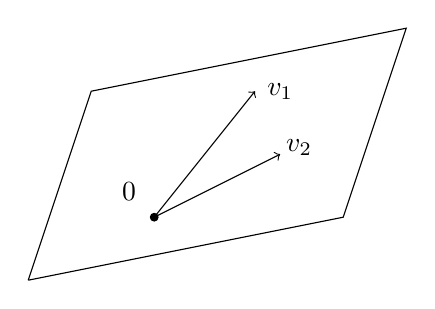
\begin{tikzpicture}[scale=0.8] 
	\draw[<-] (0,0) -- (-2,-1) node at (0,1) {$v_1$};
	\draw[->] (-2,-1) -- (-0.4,1) node at (0.3,0.1) {$v_2$};
	\fill (-2,-1) circle (2pt) node at (-2.4,-0.6) {$0$};	
	\draw (-4,-2) -- (1,-1) -- (2,2) -- (-3,1) -- (-4,-2);
	\end{tikzpicture}
	\end{center}
\end{example}\vsp

\begin{definition}
Let $v_1,\dots,v_n$ be vectors in $V$. Then the set of all linear combinations of $v_1,\dots,v_n$ is called the \emph{linear span} of $v_1,\dots,v_n$. This is denoted by Sp$(v_1,\dots,v_n)$.	
\end{definition}\vsp

\begin{proposition}
For any $v_1,\dots,v_n \in V$ the linear span Sp$(v_1,\dots,v_n)$ is a vector space of $V$. 
\end{proposition}
\begin{proof}
Again, by Prop 10.2 we need only to check that Sp$(v_1,\dots,v_n)$ is closed under $+$ and $(\times$ by scalars).	 

Indeed 
\begin{align*}
  &\lambda_1v_1 + \dots + \lambda_nv_n + (\mu_1v_1 + \dots + \mu_nv_n)\\
  &= (\lambda_1+ \mu_1)v_1  + \dots + (\lambda_n + \mu_n)v_n
\end{align*}
Also for $\mu \in F$ we have $\mu(\lambda_1v_1 + \dots + \lambda_nv_n) = (\mu_1v_1)v_1 + \dots + (\mu_n\lambda_n)v_n$.
\end{proof}

\emph{Remark.} 
$b =(b_1,\dots,b_n)^t \in F^n$. 
\emph{When is $b$ an element of Sp$(v_1,\dots,v_n)$, where $v_i \in F^n$?}

Consider the $m \times n$ matrix 
\[
  A = \begin{pmatrix}
 | & & |\\
 v_1 & \dots & v_n \\
 | && |	
 \end{pmatrix}
\]
$b \in \mathrm{Sp}(v_1,\dots,v_n)$  if and only if $b = x_1v_1 + \dots x_nv_n$. Equivalently, 
\[
  \begin{pmatrix}
 b_1 \\ \vdots \\ v_n	
 \end{pmatrix} = \begin{pmatrix}
 | & & |\\
 v_1 & \dots & v_n \\
 | && |	
 \end{pmatrix}\begin{pmatrix}
 x_1 \\ \vdots \\ x_n	
 \end{pmatrix}
 = Ax
\]
for some $x \in F^n$.\\

\begin{example}
$V = \R^2$. Consider 
\[
  v_1 = \begin{pmatrix}
 1 \\ 2 \\ 3	
 \end{pmatrix},\quad 
 v_2 = \begin{pmatrix}
 -1 \\ 0 \\ 1	
 \end{pmatrix},\quad 
 v_3 = \begin{pmatrix}
 3 \\ 1 \\ -1	
 \end{pmatrix}
\]
\emph{What is $Sp(v_1,v_2,v_3)$?}

Using the remark, we know that $b \in \mathrm{Sp}(v_1,v_2,v_3)$ if and only if $b = Ax$ has a solution. 

The augmented matrix of $Ax = b$ is this: 
\[
\begin{amatrix}{3}
  1 & -1 & 	3 & b_1\\
  2 & 0 & 1 & b_2\\
  3 & 1  & -1 & b_3
  \end{amatrix}
\]
Using Gaussian elimination we get
\[
  \longrightarrow \begin{amatrix}{3}
  	1 & -1 & 3 & b_1\\
  	0 & 2 & -5 & b_2-2b_1\\
  	0 & 0 & 0 & b_1 - 2b_2 + b_3
  \end{amatrix}
\]
\[
    \longrightarrow \begin{amatrix}{3}
  	1 & -1 & 3 & b_1\\
  	0 & 2 & -5 & b_2-2b_1\\
  	0 & 4 & -10 & b_3 - 3b_1
  \end{amatrix}
\]

If $b_1-2b_2 + b_3\neq 0$, then on solutions. If $b_1 - 2b_2 + b_3 = 0$, we have solutions (one free variable $\implies$ infinitely many). 

Conclusion: $b \in \mathrm{Sp}(v_1,v_2,v_3)$ if and only if $b_1 - 2b_2 + b_3 = 0$. In other words, Sp$(v_1,v_2,v_3)$ is a plane in $\R^3$ given by the equation $x_1 - 2x_2 + x_3 = 0$. 
\end{example}\vsp


\begin{example}
Same $v_1,v_2$ but now let $v_3 = \begin{pmatrix}
 3 \\ 1\\ 0	
 \end{pmatrix}$. 
 
 \emph{What is $Sp(v_1,v_2,v_3)$?}
 
 We need to solve $Ax = b$, where the augmented matrix is 
 \[
\begin{amatrix}{3}
  1 & -1 & 	3 & b_1\\
  2 & 0 & 1 & b_2\\
  3 & 1  & 0 & b_3
  \end{amatrix}
\]
Once again, follow the same procedure: 
 \[\longrightarrow 
\begin{amatrix}{3}
  1 & -1 & 	3 & b_1\\
  0 & 2 & -5 & b_2-2b_1\\
  0 & 4  & -9 & b_3 -3b_1
  \end{amatrix}
\]
 \[\longrightarrow 
\begin{amatrix}{3}
  1 & -1 & 	3 & b_1\\
  0 & 2 & -5 & b_2-2b_1\\
  0 & 0  & 1 & b_1 - 2b_2 + b_3
  \end{amatrix}
\]

The system has a solution for any choice of $b_1,b_2,b_3$ (and there is exactly one solution!) So $\mathrm{Sp}(v_1,v_2,v_3) = \R^3$. 	
\end{example}\vsp


\begin{definition}
Let $V$ be a vector space over $F$, and let $W \subset V$ be a subspace. If $W = \mathrm{Sp}(v_1,\dots,v_n)$, then $v_1,\dots,v_n$ is called a \emph{spanning set} for $W$. Then we say that $v_1,\dots,v_n$ spans $W$. 	
\end{definition}\vsp

\begin{example}
The vectors $e_1 = (1,0,\dots,0),\dots,e_n = (0,0,\dots,1)$ span $F^n$. Indeed $(x_1,\dots,x_n) =  x_1e_1 + \dots + x_ne_n$. 

Go back to the first example... The plane $x_1 - 2x_2 + x_3 = 0$ is Sp$(v_1,v_2,v_3)$. In fact, this plane is also Sp$(v_1,v_2)$. The reason for this is that $v_3$ is a linear combination of $v_1$ and $v_2$. Indeed 
\[
  v_3 = \begin{pmatrix}
 3 \\ 1 \\ -1	
 \end{pmatrix},\quad 
 v_1 = \begin{pmatrix}
 1 \\ 2\\ 3	
 \end{pmatrix},\quad 
 v_2 = \begin{pmatrix}
 -1 \\ 0 \\ 1	
 \end{pmatrix}
\]
\[
  v_3 = \frac{1}{2}v_1 - \frac{5}{2}v_2
\]
Therefore $\lambda_1v_1 +\lambda_2v_2 + \lambda_3v_3 = (\lambda_1 + \frac{\lambda_3}{2})v_1 + (\lambda_2 - \frac{5}{2}\lambda_3)v_2$. 
\end{example}


\begin{definition}\lecturemarker{26}{Dec} 
Let $V$ be a vector space over $F$. Then vectors $v_1,\dots,v_n$ are \emph{linearly dependent} if there exists $\lambda_1,\dots,\lambda_n \in F$ not all equal to zero such that $\lambda_1v_1 + \dots + \lambda_nv_n = 0 \in V$.
\end{definition}

The motivation for this is when $v_1,\dots,v_n$ are linearly dependent, one of these vectors is a linear combination of all the others.

Indeed some $\lambda_i \neq 0$. To fix ideas assume $\lambda_1 \neq 0$. Then 
\[
  v_1 = -\frac{1}{\lambda_1}(\lambda_2v_2 + \dots + \lambda_nv_n)
\]
In this case Sp$(v_1,\dots,v_n) = \mathrm{Sp}(v_2,\dots,v_n)$. \\

\begin{definition}
$v_1,\dots,v_n$j are \emph{linearly independent} if the only way to write the zero vector as a linear combination of $v_1,\dots,v_n$ is with all coefficients equal to $0$, i.e. if $0 = \lambda_1v_1 + \dots\lambda_nv_n \implies \lambda_1 = \dots = \lambda_n = 0$. 
\end{definition}\vsp

\emph{Remarks.}~\\[.1cm]
(i) One vector $v \in V$ is linearly independent (assuming $v \neq 0$, i.e. $v$ is a non-zero vector)

(ii) Two vectors $v_1,v_2 \in V$ are linearly independent if and only if they are not proportional. $\lambda_1v_1 + \lambda_2v_2 = 0$. If $\lambda_1 \neq 0$, then $v_1 = -\frac{\lambda_2}{\lambda_1}v_2.$ If $\lambda_2 \neq 0$, then $v_2 = -\frac{\lambda_1}{\lambda_2}v_1$. 

(ii) Let $V = F^m$. Suppose $v_1,\dots,v_n \in V$. Consider the $m \times n$ matrix $A$ such that $v_1,\dots,v_n$ are the columns of $A$:
\[
  A = \begin{pmatrix}
 | & \dots & |\\
 v_1 & \dots & v_n\\
 | & \dots & |	
 \end{pmatrix}
\]

Then $v_1,\dots,v_n$ are linearly dependent if and only if the equation $Ax = 0$ has a non-zero solution. 

Clearly $x = (x_1,\dots,x_n)^t$ is a solution, then $x_1v_1 + \dots + x_n v+n = 0$. If $Ax = 0 \implies x = 0$, then $v_1,\dots,v_n$ are linearly independent. If $ax = 0$ has a non-zero solution then $v_1,\dots,v_n$ are linearly dependent.\\

\begin{proposition}
Any subset of a set of linearly independent set of vectors is linearly independent.	
\end{proposition}
\begin{proof}
Suppose that $v_1,\dots,v_n$ are linearly independent. Without loss of generality, we can assume that our subset is $v_1,\dots,v_k$ for some $k \in n$. If $v_1,\dots,v_k$ are linearly dependent, then we can find $\lambda_1,\dots,\lambda_n \in F$ (scalars) such that $\lambda_1v_1 + \dots \lambda_kv_k = 0$, and not all of $\lambda_1,\dots,\lambda_k$ are $0$. 

Consider
\[
  \lambda_1v_1 + \dots + \lambda_kv_k + 0v_{k+1} + \dots + 0v_n = 0
\]
This is a linear combination of all $v_1,\dots,v_n$ with at least one non-zero coefficient. Hence $v_1,\dots,v_n$ are linearly dependent. This is a contradiction, therefore $v_1,\dots,v_k$ are linearly independent.
\end{proof}\vsp

\begin{proposition}
	Let $V$ be a vector space over $F$. Let $v_1,\dots,v_n \in V$. Then $v_1,\dots,v_n$ are linearly dependent if and only if one o them is a linear combination of the others.
\end{proposition}

\begin{proof}
Suppose $v_1,\dots,v_n$ are linearly dependent. Then we can find $\lambda_1,\dots,\lambda_n$ such that $\lambda_1v_1 + \dots + \lambda_nv_n = 0$ and one of $\lambda_i$s, say $\lambda_1$ is non-zero. Then 
\[
  v_1 = -\frac{1}{\lambda_1}(\lambda_2v_2 + \dots \lambda_nv_n)
\]
Conversely if $v_1 = \mu_2v_2 + \dots \mu_nv_n$ where $\mu_i$'s $\in F$, then 
\[
  (-1)v_1 + \mu_2v_2 + \dots + \mu_nv_n = 0
\]
$(-1) \neq 0$, so at least one coefficient is non-zero. Hence $v_1,\dots,v_n$ are linearly dependent. 
\end{proof}\vsp


\begin{definition}
Let $V$ be a vector space over $F$. A set of vectors $v_1,\dots,v_n \in V$ is called a \emph{basis} of $V$ if 

(i) $V = \mathrm{Sp}(v_1,\dots,v_n)$

(ii) $v_1,\dots,v_n$ are linearly independent.
\end{definition}

In other words, every vector of $V$ is a linear combination of $v_1,\dots,v_n$ (this is property (i)), and and no $v_i$ is a linear combination of $v_1,\dots,v_{i-1},v_{i+1},\dots,v_n$. \\

\begin{examples}

(i) $V = F^n$. Then $e_1 = (1,0,\dots,0), e_2 = (0,1,\dots,0), \dots, e_n = (0,0,\dots,1)$ is a basis of $F^n$. 

$(x_1,\dots,x_n) = x_1e_1 + \dots x_ne_n$, so Sp$(e_1,\dots,e_n) = F^n$. Clearly $e_1,\dots,e_n$ are linearly independent: $\lambda_1e_1 + \dots + \lambda_ne_n = 0$. This says $(\lambda_1,\lambda_2,\dots,\lambda_n)$ is the zero vector. Hence $\lambda_i = 0,\, i = 1,\dots,n$. So $e_1,\dots,e_n$ is a basis. 


\begin{warning}
There are many other bases! e.g. $R^2$ has a basis $(1,1)$ and $(1,3)$. Indeed $(1,1)$ and $(1,3)$ are not proportional, hence are linearly independent. 
\end{warning}


(ii) Let $V$ be a vector space of polynoials in $x$ of degree at most $d$. 
\[
  V = \{f_dx^d + \dots + f_1x_1 + f_0 ~|~ f_i \in F\}
\]
$f_dx^d + \dots + f_0$ is a linear combination of $1,x,\dots,x^d$ with coefficients $f_0,\dots,f_d$. But $1,x,\dots,x^d$ are linear indepdent vectors of $V$. So suppose $lambda_0 + \lambda_1x + \dots + \lambda_dx^d =0$ (the zero polynomial.) Conclusion: $1,x,\dots,x^d$ is a basis of the vector space of polynomials of degree $\leq d$. 

Other basis exist: e.g. $1,x+1, x^2 + 1,\dots,x^d + 1$ is also a basis.
\end{examples}\vsp


\emph{Remark.} Let $V = F^n$. Then $v_1,\dots,v_n \in V$ form a basis of $V$ if and only if the matrix equation $Ax = 0$ has only one solution $x = 0$. Here 
\[
  A =\begin{pmatrix}
 | & \dots & |\\
 v_1 & \dots & v_n\\
 | & \dots & |	
 \end{pmatrix}
\]

We've seen that $v_1,\dots,v_n$ are linearly independent if the only solution is the zero solution. We still need to justify that if $Ax = 0$ has only one solution, then $v_1,\dots,v_n$ span $V$.\\

\emph{When does {\normalfont\lecturemarker{27}{12/12} }$v_1,\dots,v_n \in F^n$ form a basis?}

Consider 
\[
  A = \begin{pmatrix}
 | & & | \\ v_1 & \dots & v_n \\ | & & |	
 \end{pmatrix}
\]

Answer: $v_1,\dots,v_n$ are a basis of $F^n$ is and only if the equation $Ax = 0$, where $x= (x_1,\dots,x_n)^t$ has the unique solution $0$. Equivalently, $\det(A) \neq 0$. 
 
 $x$ is a solution $\iff x_1v_1 + \dots + x_nv_n = 0$. Hence, since $v_1,\dots,v_n$ are linearly independent the only solution is $x_1 = \dots = x_n = 0$. $\det(A) \neq 0 \implies A^{-1}$ exists. 
 
 To prove that $F^n = \mathrm{Sp}(v_1,\dots,v_n)$, we must observe that any vector $b = (b_1,\dots,b_n)^t$ can be written as $b = Ac$ for some $c = (c_1,\dots,c_n)^t$. This is so because $b = Ac$ says that $b = c_1v_1 + \dots + c_nv_n$. Take $c = A^{-1}b$. Then $b = Ac$ as required.\\
 
 \begin{proposition}
 %10.7
 Let $V$ be a vector space over $G$ with a basis $\{v_1,\dots,v_n\}$. Then any vector $v \in V$ is uniquely written as $v = \lambda_1v_1 + \dots + \lambda_nv_n$. 	
 \end{proposition}
 \begin{proof}
 Suppose that 
 \[
  v = \lambda_1v_1 + \dots + \lambda_nv_n
\]
and
\[
  v = \mu_1v_1 + \dots \mu_nv_n
\]
Then $(\mu_1-\lambda_1)v_1 + \dots + (\mu_n - \lambda_n)v_n = 0$. Since $v_1,\dots,v_n$ is a basis, these vectors are linearly independent. By the definition of linear independence, we must have $\lambda_1 = \mu_1,\dots,\lambda_n = \mu_n$. 
 \end{proof}
 
 \begin{theorem}
 Let $V$ be a vector space over $F$. Suppose that $\{v_1,\dots,v_n\}$ and $\{w_1,\dots,w_m\}$ are both bases of $V$. Then $m = n$. 	
 \end{theorem}
 
 - So any basis of $V$ has the same number of elements. 
 
 \begin{proof}
 $V = \mathrm{Sp}(w_1,\dots,w_m)$ and $V = \mathrm{Sp}(v_1,\dots,v_n)$. Thus we can write: 
 \[
  v_i = \sum_{j=1}^n a_{ij}w_j \quad \text{ for some } a_{ij} \in F
\]
Let $A$ be the $m \times n$ matrix with entries $a_{ij}$. 

Similarly we write: 
\[
  w_j = \sum_{k=1}^m b_{kj}v_k \quad \text{ for some } b_{jk} \in F
\]
Therefore, 
\[
  v_i - \sum_{j=1}^n a_{ij} \cdot \sum_{k=1}^m b_{jk} v_k \tag{$*$}
\]
By Proposition 10.7, there is only one way of writing $v_i$ as a linear combination of $v_1,\dots,v_n$, namely as $v_i = 0v_1 + \dots + 1\cdot v_i + \dots + 0v_n$. 

Hence RHS of $(*)$ is simply $v_i$. In otherwords, we have 
\[
  \sum_{j=1}^n \sum_{k=1}^m a_{ij}b_{jk} = 1 \quad \text{ if } k =i
\]
and 
\[
  \sum_{j=1}^n \sum_{k=1}^m a_{ij}b_{jk} = 0 \quad \text{ if } k \neq i
\]
The framed expressions are the entries of $AB$. 

The $ii$ entry of $AB$ is the first sum, that is 
\[
  \sum_{j=1}^n \sum_{k=1}^m a_{ij}b_{jk} = 1
\]
The $1k$-entry of $AB$, $i \neq k$, is the second sum, that is 
\[
  \sum_{j=1}^n\sum_{k=1}^m a_{ij}b_{jk} = 0
\]
This means $AB = I_m$, the identity matrix of size $m \times m$. 

By swapping $v_i$'s and $w_j$'s, we show similarly that $BA = I_n$, the identity matrix of size $n \times n$. Thus $AB = I_n$ and $BA = I_m$. 

Recall that the trace of a square matrix is the sum of the diagonal elements. 

\textbf{Fact:} Tr$(AB) = \mathrm{Tr}(BA)$. 

This is enough to finish the proof because Tr$(I_n) = n$ and Tr$(I_m) = m$. 

\emph{Proof of Fact.} The $ii$ entry of $AB$ is 
\[
  \sum_{j=1}^n a_{ij}b_{ji} \implies Tr(AB) = \sum_{i=1}^n \sum_{j=1}^n a_{ij}b_{ji}
\]
The $jj$-entry of $BA$ is 
\[
  \sum_{i=1}^m b_{ji}a_{ij}
\]
So
\begin{align*}
  Tr(BA) &= \sum_{j=1}^n \sum_{i=1}^m b_{ji} \cdot a_{ij}\\
  &= \sum_{i=1}^m \sum_{j=1}^n a_{ij}b_{ji} \\
  &= Tr(AB)
\end{align*}
The proves the fact, and hence the theorem. 
\end{proof}

\begin{definition}
	Suppose a vector space $V$ over $G$ has a basis consisting of $n$ vectors. Then $n$ is called the \emph{dimension of $V$ = dim$V$}. 
	
	If $V$ has a basis (of finitely many elements), then $V$ is called a \emph{finite-dimensional vector space}.
\end{definition}\vsp

\begin{example}
Let $V$ be the space of all polynomials in $x$ with real coefficients. 

\textbf{Claim:} $V$ is not finite-dimensional . 
\begin{proof}
Suppose that $V$ is spanned by finitely many polynomials, say $f_1(x),\dots,f_n(x)$. 

Let $d$ be a natural number so that $d > \mathrm{deg}\,f_i(x)$ with $i = 1,\dots,n$. Then $x^d$ is not a linear combination of $f_1(x),\dots,f_n(x)$. 
\end{proof}
\end{example}

\pagebreak

\begin{theorem}
Let $V$ be a vector space. Suppose that $v_1,\dots,v_n\in V$ span $V$. Then 
\begin{enumerate}
\item  dim$V\leq n$
\item There is a subset of $\{v_1,\dots,v_n\}$, which is a basis of $V$. 	
\end{enumerate}
\end{theorem}

Note that (ii) $\implies$ (i). Indeed dim$V = $ number of elements in any basis of $V$, so dim$V \leq n$, because removing some of the vectors from $\{v_1,\dots,v_n\}$ we obtain a basis of $V$. Hence (ii) $\implies$ (i). 

\begin{proof}[Proof of (ii)]
We use the \emph{casting out process}. 

Start with $v_1,\dots,v_n$. If $v_1,\dots,v_n$ are linearly independent, then $\{v_1,\dots,v_n\}$ is a basis. If $v_1,\dots,v_n$ are linearly independent [i.e. linearly dependent] then we find $\lambda_1,\dots,\lambda_n \in F$ such that $\lambda_1v_1 + \lambda_nv_n = 0$ and at least one coefficient $\lambda_i \neq 0$. Say $\lambda_n \neq 0$. Then 
\[
  v_n = -\frac{1}{\lambda_n}(\lambda_1v_1 + \dots + \lambda_{n-1}v_{n-1})
\]
Therefore $V$ is spanned by $v_1,\dots,v_{n-1}$, i.e. $V = \mathrm{Sp}(v_1,\dots,v_n) = \mathrm{Sp}(v_1,\dots,v_{n-1})$. 

Continue like this, we stop when we are met with a linearly independent set of vectors. But we ensure that these vectors span $V$. Hence we have obtained a basis of $V$.
\end{proof}









We wanted to classify \lecturemarker{29}{17/12}
all vector space of $\R^3$. dim$(\R^3) = 3$, and dim$(\{0\}) = 0$ by definition. (We define the dimension of $\{0\}$ to be zero.)

If $V \subset \R^3$ is a vector space, then dim$(V)$ can be $0,1,2,$ or $3$. If dim$(V) = 3$, then $V$ has a basis of $3$ vectors, but then it's a basis of $\R^3$. Hence $V = \R^3$.\\

\textbf{Felina.} Finally we look at an application to error-correcting codes: 

\subsektion{* Error correcting codes *}

Now $F = \F_2 = \{0,1\}$ with binary addition and multiplication. $1 + 1 = 0$. 

Consider the $n$-dimensional vector space $(\F_2)^n = \{(x_1,\dots,x_n) ~|~ x_i \in \F_2\}$. We've seen that every vector space of $(\F_2)^k$ is a vector subspace of dimension $n$ over $\F_2$, where $0 \leq m \leq n$. 

Let $v_1,\dots,v_m$ be a basis of $V$, where $m = \mathrm{dim}(V)$. We know that every vector $v \in W$ is uniquely written as 
\[
  v = \lambda_1v_1 + \dots \lambda_mv_m
\]
where $\lambda_i \in \F_2$, i.e. $\lambda_i = 0$ or $\lambda_i = 1$. 

The number of elements in $(\F_2)^n$ is $2^n$ .If $V \subset (\F_2)$ has dim$(V) = m$, then $|V| = 2^m$. 

Recall that if $v = (x_1,\dots,x_n)$ and $w = (y_1,\dots,y_n)$ in $\R^n$, then the distance between $v$ and $w$ is \[\sqrt{(x_1 - y_1)^2 + \dots + (x_n - y_n)^2}\] This doesn't work well for $\F_2$. Instead consider the \emph{Hamming distance.}\\


\begin{definition}
Let $v, w \in (\F_2)^n$. The \emph{Hamming distance}, dist$(v,w) = $ the number of $i \in \{1,\dots,n\}$ such that $v_i \neq w_i$. 	
\end{definition}

For example, dist$(v,0) = $ the number of non-zero coordinates of $v$. 

Any reasonable notion of distance should satisfy three axioms: 
\begin{enumerate}
\item dist$(v,v) = 0$
\item dist$(v,w) = \mathrm{dist}(w,v) \quad \forall v,w \in V$
\item dist$(v,w) \leq \mathrm{dist}(u,u) + \mathrm{dist}(u,w)$

(dist$(v,w)$ is always a non-negative real number.)	
\end{enumerate}

\emph{Exercise:} Check Axiom (iii). 


Error-correcting codes are used to transmit messages in such a way that a distorted message can be decoded correctly. 

Messages are first encoded into sequences of $0$ and $1$ of some length. We get, say $2^d$ possible messages, encoded into sequences of length $1$. 

\textbf{The idea of error correction in the case of $1$ error:}

\subsubsektion{The Hamming code}

We are going to realise $2^d$ messages as elements of a vector subspace of $(\F_2)^n$, $V \subset (\F_2)^n$. 

The construction: consider the matrix of size $m \times 2$ such that the columns are all vectors with coordinates $0$ and $1$ except the all-$0$ vector. E.g. if $m = 3$, 
\[
  A =\begin{pmatrix}
1 & 0 & 0 & 1 & 1 & 0 & 1\\
0 & 1 & 0 & 1 & 0 & 1 & 1\\
0 & 0 & 1 & 0 & 1 & 1 & 1 	
\end{pmatrix}
\]

Define $V = \{x \in \F^{2^m -1} ~|~ Ax = 0\}$. 

Crucial property: Suppose $v,w \in V, v \neq w$. We transmit $v,w$ and receive $v', w'$. We assumed that at most one error occurs during transmission, so either $v' = v$ or dist$(v,v') = 1$ and similarly for $w$. 

The main point is that the set of $v' \in (\F_2)^n$ such that dist$(v,v') \leq 1$ does not overlap with the set of $w' \in (\F_2)^n$ such that dist$(w,w') \leq 1$. Once we've proved that we know that the closest vector to $v'$ is the original vector $v$. 

In fact for any $v,w \in V$, dist$(v,w) \geq 3$ if $v\neq w$. 
%%% LOOK AT FB NOTES!!!!!

\begin{proof}
	\[
  A =\begin{pmatrix}
1 & 0 & 0 & 1 & 1 & 0 & 1\\
0 & 1 & 0 & 1 & 0 & 1 & 1\\
0 & 0 & 1 & 0 & 1 & 1 & 1 	
\end{pmatrix}
\]
If dist$(v,w) = 1$, then $v-w$ has exactly one non-zero coordinate. But $V$ has no such vectors! (The matrix has no zero columns). 

If dist$(v,w) = 2$, then $v-w$ has exactly two non-zero co-ordinates, but there are non such vectors in $V$ (The matrix has no two identitcal columns). Hence dist$(v,w) \geq 3$, if $v \neq w$ in $V$. 
\end{proof}


\begin{proof}[Proof of the crucial property]
If $v' = w'$, dist$(v,v') \leq 1$ and dist$(w,w') \leq 1$. Then by the triangle inequality
\[
  \mathrm{dist}(v,w) \leq \mathrm{dist}(v,v') + \mathrm{dist}(w,w') \leq 2
\]
a contradiction.
\end{proof}


The decoding is very easy: 

Let $v \in V$, so that $Av = 0$. Let $v'$ be the received vector. We assume that $v' = v$ or $v' = v + e$, where $e$ has exactly one non-zero coordinate. 

Recipe for decoding. 

$Av'$ is a column vector with $3$ co-ordinates. If $Av' = 0$ then $v' = v$ and no errors occurred. Otherwise $Av'$ is a column of $A$. The position of $Av'$ in $A$ is the coordinate where the error has occurred. Hence we can recover $v$.

\textbf{Summary} 

$V$ is a vector space of dimension 
\[
  \mathrm{dim}V = 2^m - 1 - m
\]
\emph{Exercise:} Show that the system of linear equations that defines $V$ has this number of free variables. 

Hence $|V| = 2^{2^m - 1- m}$, with $V \subset (\F_2)^{2^m-1}$.




Final Comment: The whole space $(\mathbb{F}_2)^{2^m}$ is the disjoint union of \emph{Hamming spheres} of radius, i.e. $(\mathbb{F}_2)^{2^m-1}$ is the disjoint union of $\{a' ~|~ \mathrm{dist}(n-v)\}$ over all $v \in V$. In other words each vector of $(\mathbb{F}_2)^{2^m-1}$ is at the distance $1$ from vector in $v$, which is unchanged. %FB COMMENTS

\theend
%\begin{center}
%\emph{The story continues in \href{https://wwwf.imperial.ac.uk/~kb514/M1P2.pdf}{M1P2 Algebra I}...}	
%\end{center}
%

\pagebreak


\end{document}
